\documentclass[11pt]{amsart}
\usepackage{geometry}                % See geometry.pdf to learn the layout options. There are lots.
\geometry{letterpaper}                   % ... or a4paper or a5paper or ... 
%\geometry{landscape}                % Activate for for rotated page geometry
%\usepackage[parfill]{parskip}    % Activate to begin paragraphs with an empty line rather than an indent
\usepackage{graphicx}
\usepackage{amssymb}
\usepackage{epstopdf}
\usepackage{booktabs}
\usepackage{wasysym}
                  % ... or a4paper or a5paper or ... 
\usepackage{multirow}
\usepackage{siunitx}
\usepackage{color, colortbl}
\usepackage{xcolor}
\usepackage{adjustbox}

\DeclareGraphicsRule{.tif}{png}{.png}{`convert #1 `dirname #1`/`basename #1 .tif`.png}
\definecolor{Bittersweet}{rgb}{1.0, 0.44, 0.37}

\title{How can we assess the accuracy of a Bayesian Network?}
\author{The Author}
%\date{}                                           % Activate to display a given date or no date

\begin{document}
\maketitle

\section{Preamble - Assumptions}
\begin{enumerate}
\item We can create a multi-agent simulation that represents some simple criminal scenario, a possible theft. The frequencies at which events occur in this simulation is in part due to interaction of agents with their surroundings, and in another part due to randomly generated numbers that represent internal `mental' factors of the agent. The events in this crime scenario can be subdivided into two classes: hypothesis events, and evidence events.
\item We can create a Bayesian Network that represents this multi-agent simulation that corresponds exactly to the frequencies we have observed in the simulation. We create this network by running the simulation for 2000 times, and storing which events took place in each run. On this data, we used a K2 algorithm to create a Bayesian Network (given certain temporal constraints).
\end{enumerate}


\section{Introduction}
In this section, I have disturbed the CPTs of an ``objective'' Bayesian Network (see preamble). I disturb the CPTs with 3 different processes, that might all represent human approaches to reasoning with probabilities. I then present the effect of these disturbances in the CPTs, on the ability of the disturbed BNs to get similar outcomes to the ``objective'' Bayesian Network. 

 The original BN was created with certain temporal constraints (ordering) with the K2 algorithm, with CPTs that exactly represent the underlying probabilistic structure of the multi-agent simulation that the BN must represent.

The BN was disturbed by three different processes.

\begin{enumerate}

\item Process 1 is straightforwardly losing precision by changing the rounding in the CPTs. Rounding took place from 5 decimals (very precise) to 0 decimals (turn the number to 0 or 1, obviously this resulted in a BN that could not be used (incompatible). This is to see if the float errors in BNs matter in case of this simulation.

\item Process 2 is rounding to arbitrary intervals - these intervals were chosen to represent human intuition, like 8ths, 4ths, 3rds and even halves (so the only numbers allowed in the cpt in that last one, are 0, 0.5 and 1). This should reflect relatively normal human reasoning - if we don't have exact numbers, we want to estimate to some arbitrary degree. And in this case I wanted to see how granular our estimation needs to be in order to come to a similar conclusion as the K2 network. Note - this only affects the cpt, we assume that we can think of the same structure as the cpt (ie we are able to identify all the independence/dependence relations).

\item Process 3 is disturbing the cpts with random normal noise, representing the effect of confusion about directionality/causality in the network. The standard deviation of the normal noise is increased (mean at 0), to represent greater confusing about the direction of the network. Here, in the tables below we look at the \% of times that the disturbed network corresponds with the original network.
\end{enumerate}

\subsection{The Weak and the Strong Interpretation of Bayesian Networks}
There are 2 ways of viewing the use of BNs, which I will call the weak view and the strong view. In the weak view, probabilities are subjective estimations, and furthermore, it doesn't exactly matter what these probabilities are, as long as they help us to reason with the evidence. In this view (see Taroni), BNs can help us to reason with complex structures of evidence and hypotheses, without looking much at the numbers, but more at which hypothesis is supported: does some piece of evidence support some hypothesis in some way, even across many different causal connections? However, the exact strength of the probabilities in the CPT does not matter, its not that relevant. The numbers are only relevant insofar as they can cause us to prefer one hypothesis over another. We only care about the direction that evidence leans towards - towards H1 or towards H0?

In the strong view, BNs are also subjective, but here the numbers do actually matter. We can make precise claims or estimations about probabilities, and the numbers actually represent evidence strength in a relatively precise manner. We cannot only look at the direction - the precision/numbers are informative as well. We need to care about the numbers, not just a binary (supports H1 vs H0), but if we see that support for H1 is 0.80, that means something meaningfully different from support for H1 = 0.99.

Hence, here I investigate this weak vs strong view, by looking at both the `support direction' - what, for each node in the original network, is the hypothesis that they support (H1 or H0), and does the disturbed network support that same hypothesis, under all processes of disturbance?
The other thing is the `precision' - to what extent does the disturbed network diverge from the actual probability value of H1 in every node in the network? How big is this disturbance?

\subsection{Why not just use...}
Sensitivity Analysis?

vague idea: it shows the upper and lower boundaries for change, but not a cognitive process that might be at play in assigning the CPTs.

\section{Conclusion and Discussion}

The network is relatively robust against disturbances, especially in the weak view, where in almost all cases for any disturbance, the same hypothesis is supported as the original network. In the strong view, probabilities diverge a lot, hence I would not trust a judge with a 99\% estimate.

The process 2 is promising, shows that even with not very granular numbers we can still show some type of evidence strength. 

Also my simulation is not interesting enough, I will change some of the original probabilities so that these numbers might become more interesting (the disturbed house, spotted nodes do not add anything to the story while they should, since the broken lock evidence is too strong).

\clearpage
\section{Results Plots}
 {\tiny Note - there's a slight position dodge in the lines for certain images, otherwise they would overlap. A value of NA in the weak-view plots means that the BN is inconsistent.}
\begin{figure}[htbp]
\begin{center}
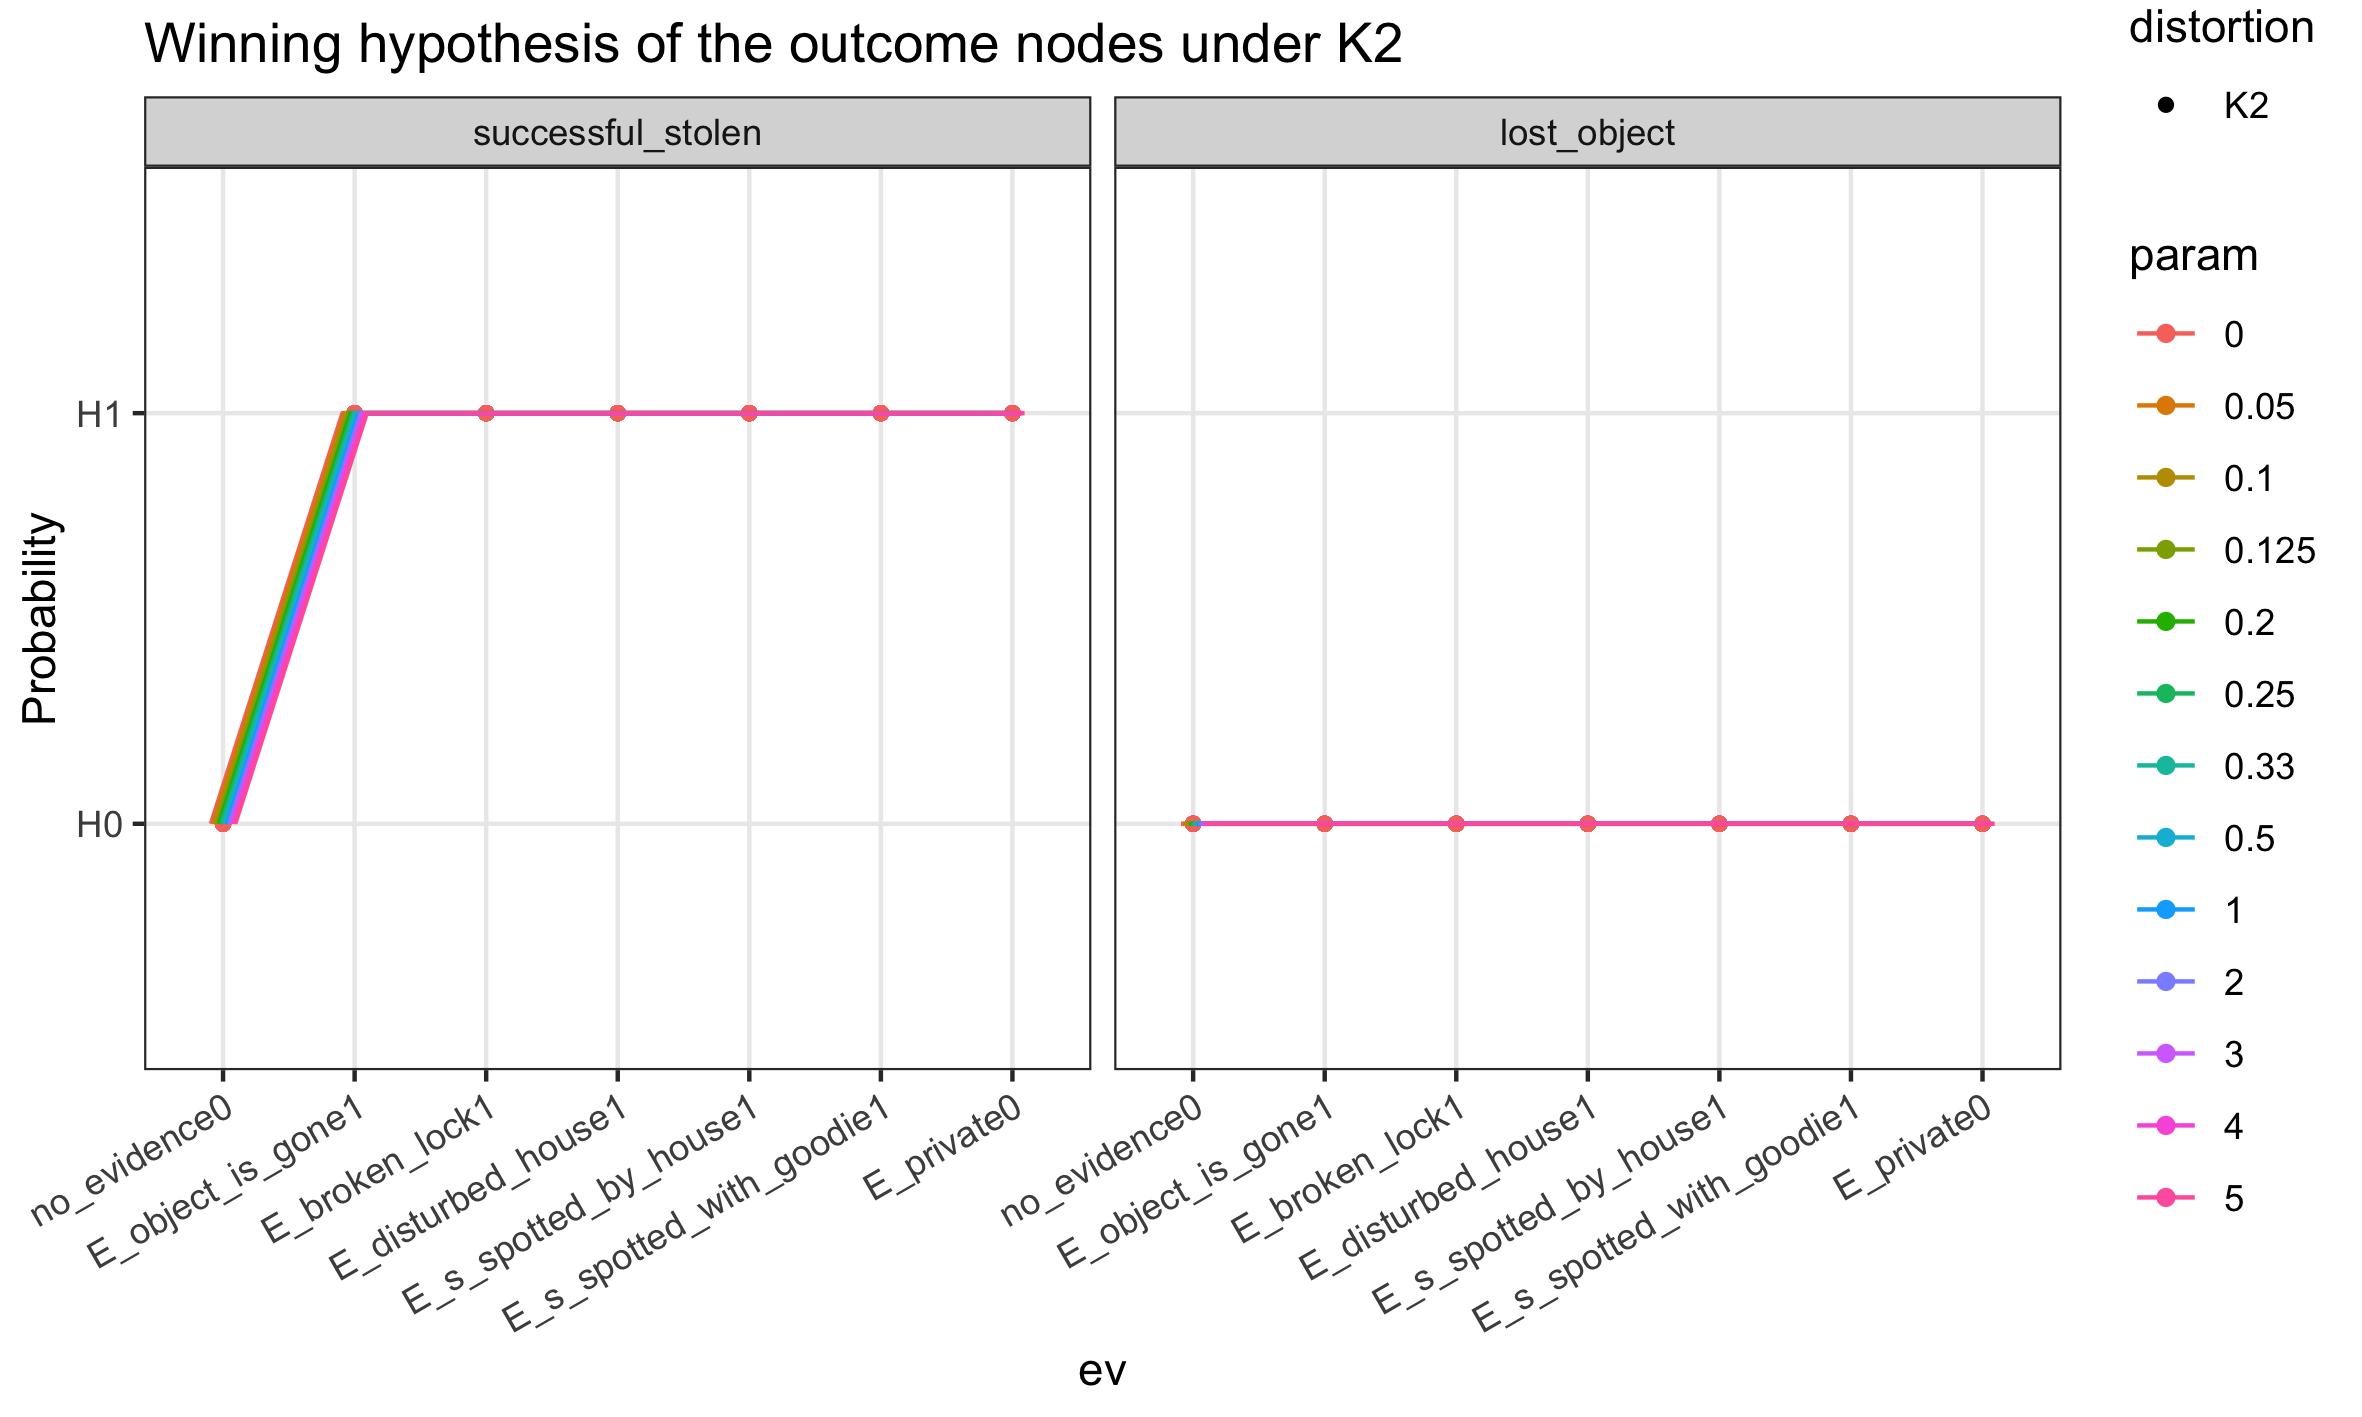
\includegraphics[scale=0.15]{images/K2Weak.png}
\label{default}
\end{center}
\end{figure}
\begin{figure}[htbp]
\begin{center}
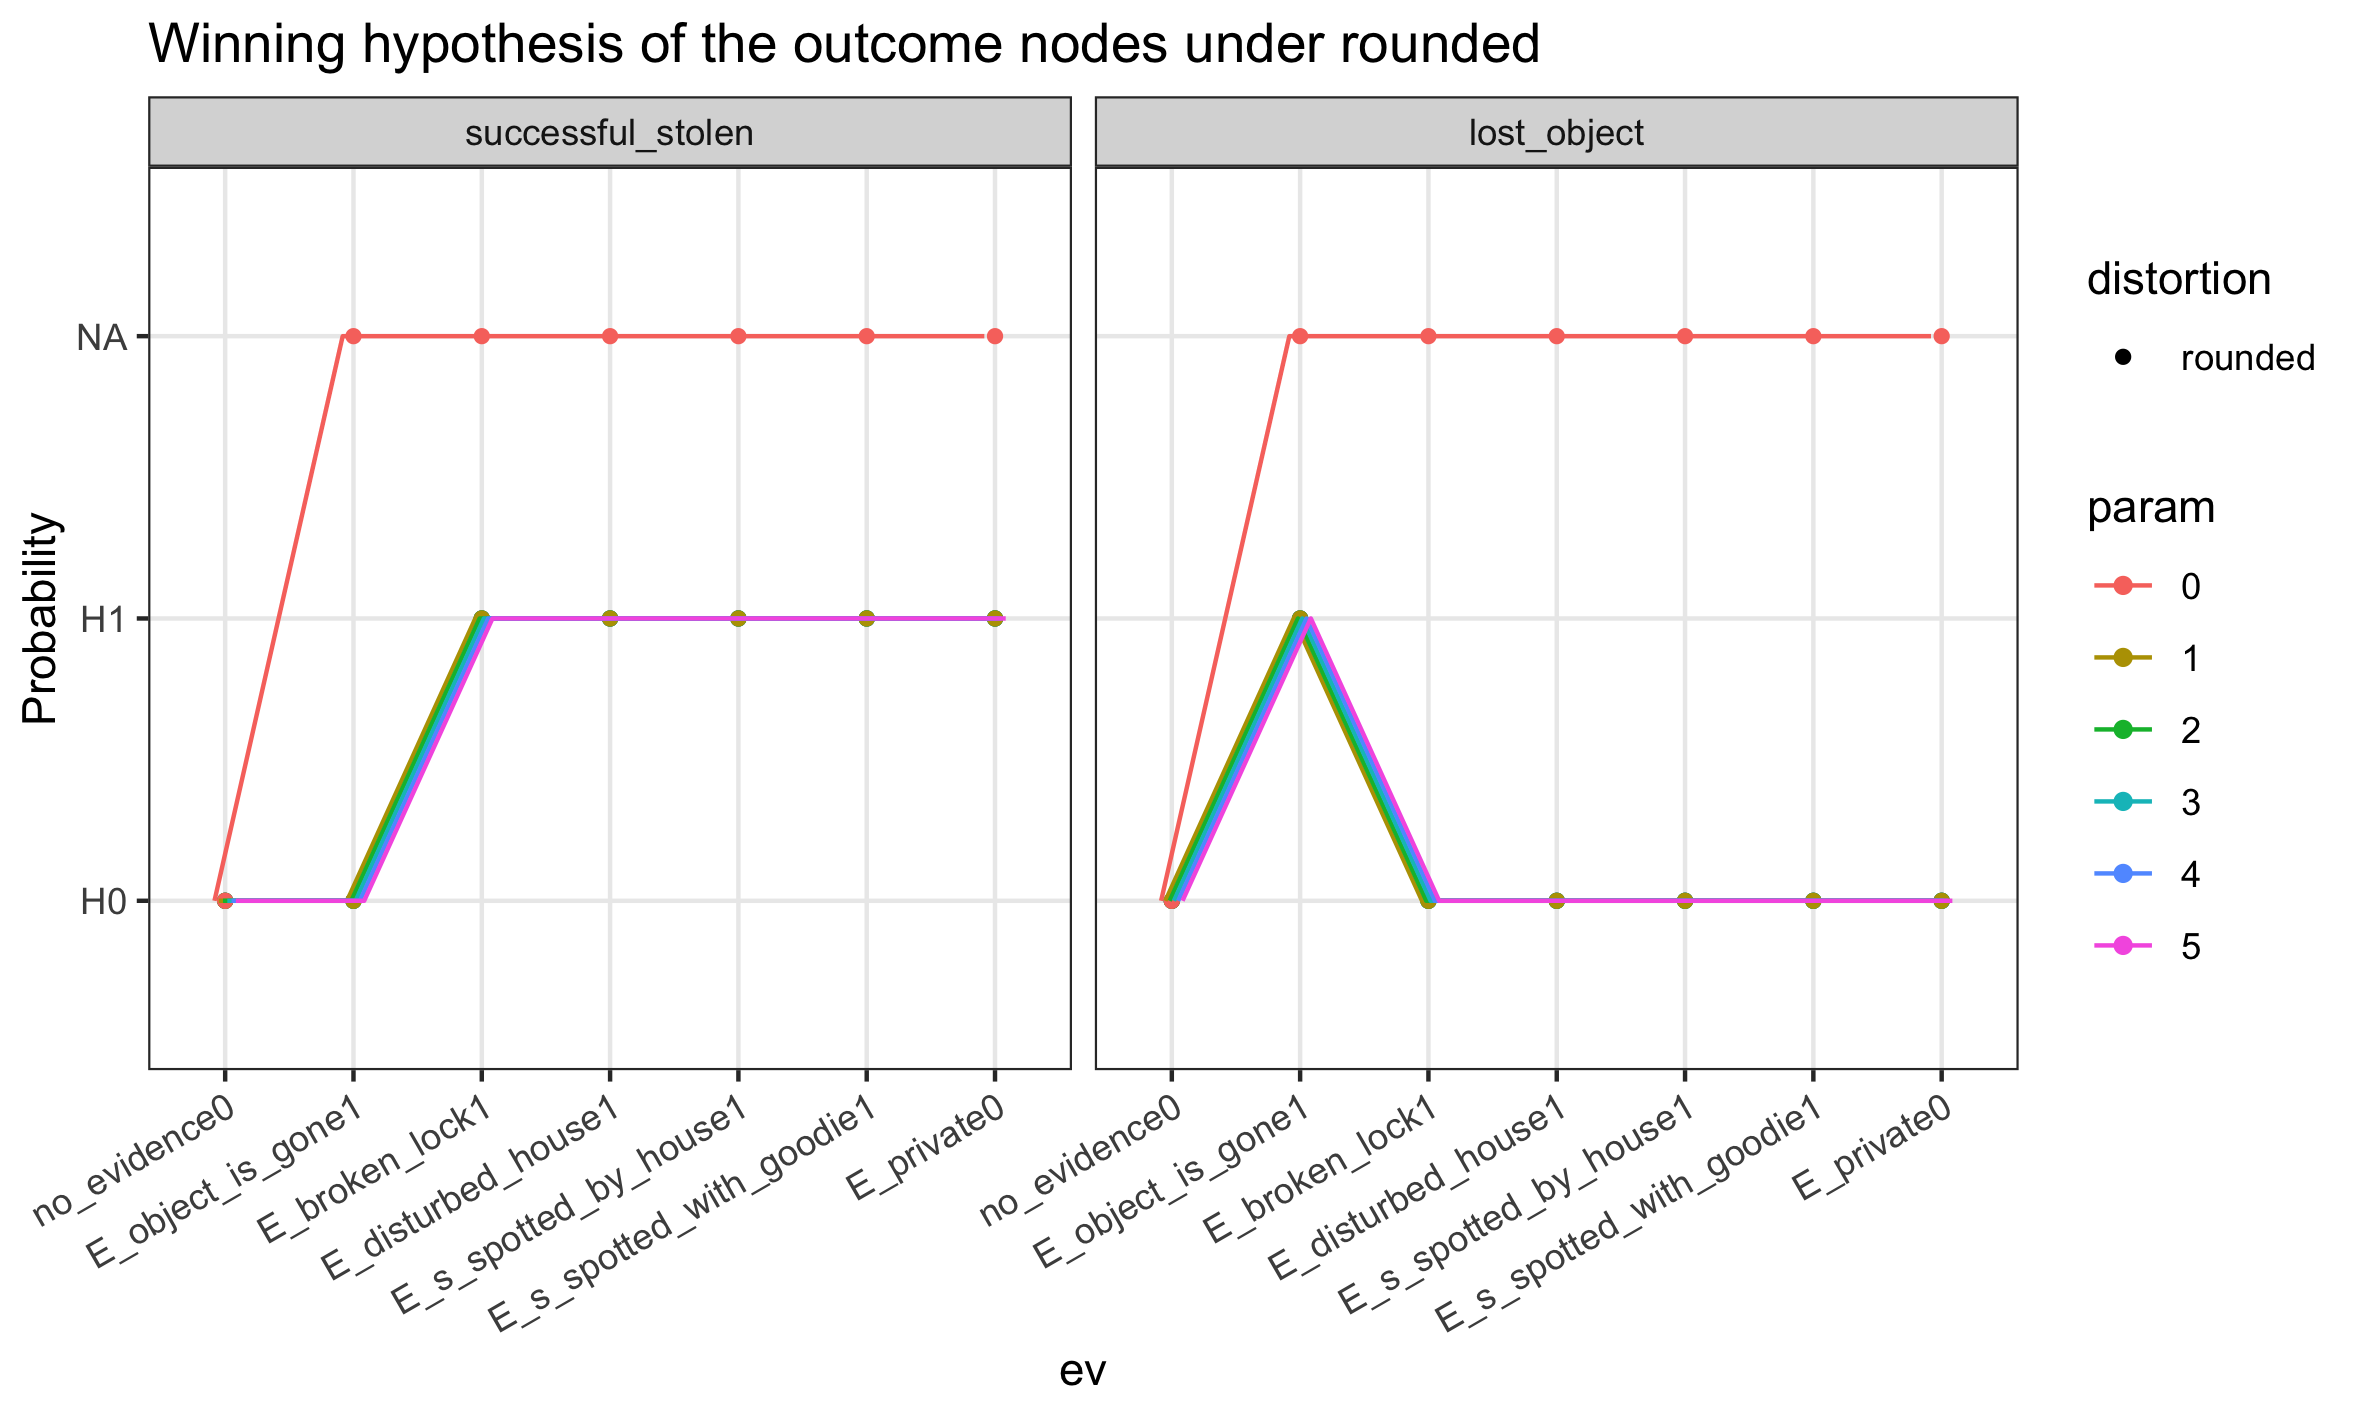
\includegraphics[scale=0.15]{images/roundedWeak.png}
\label{default}
\end{center}
\end{figure}
\begin{figure}[htbp]
\begin{center}
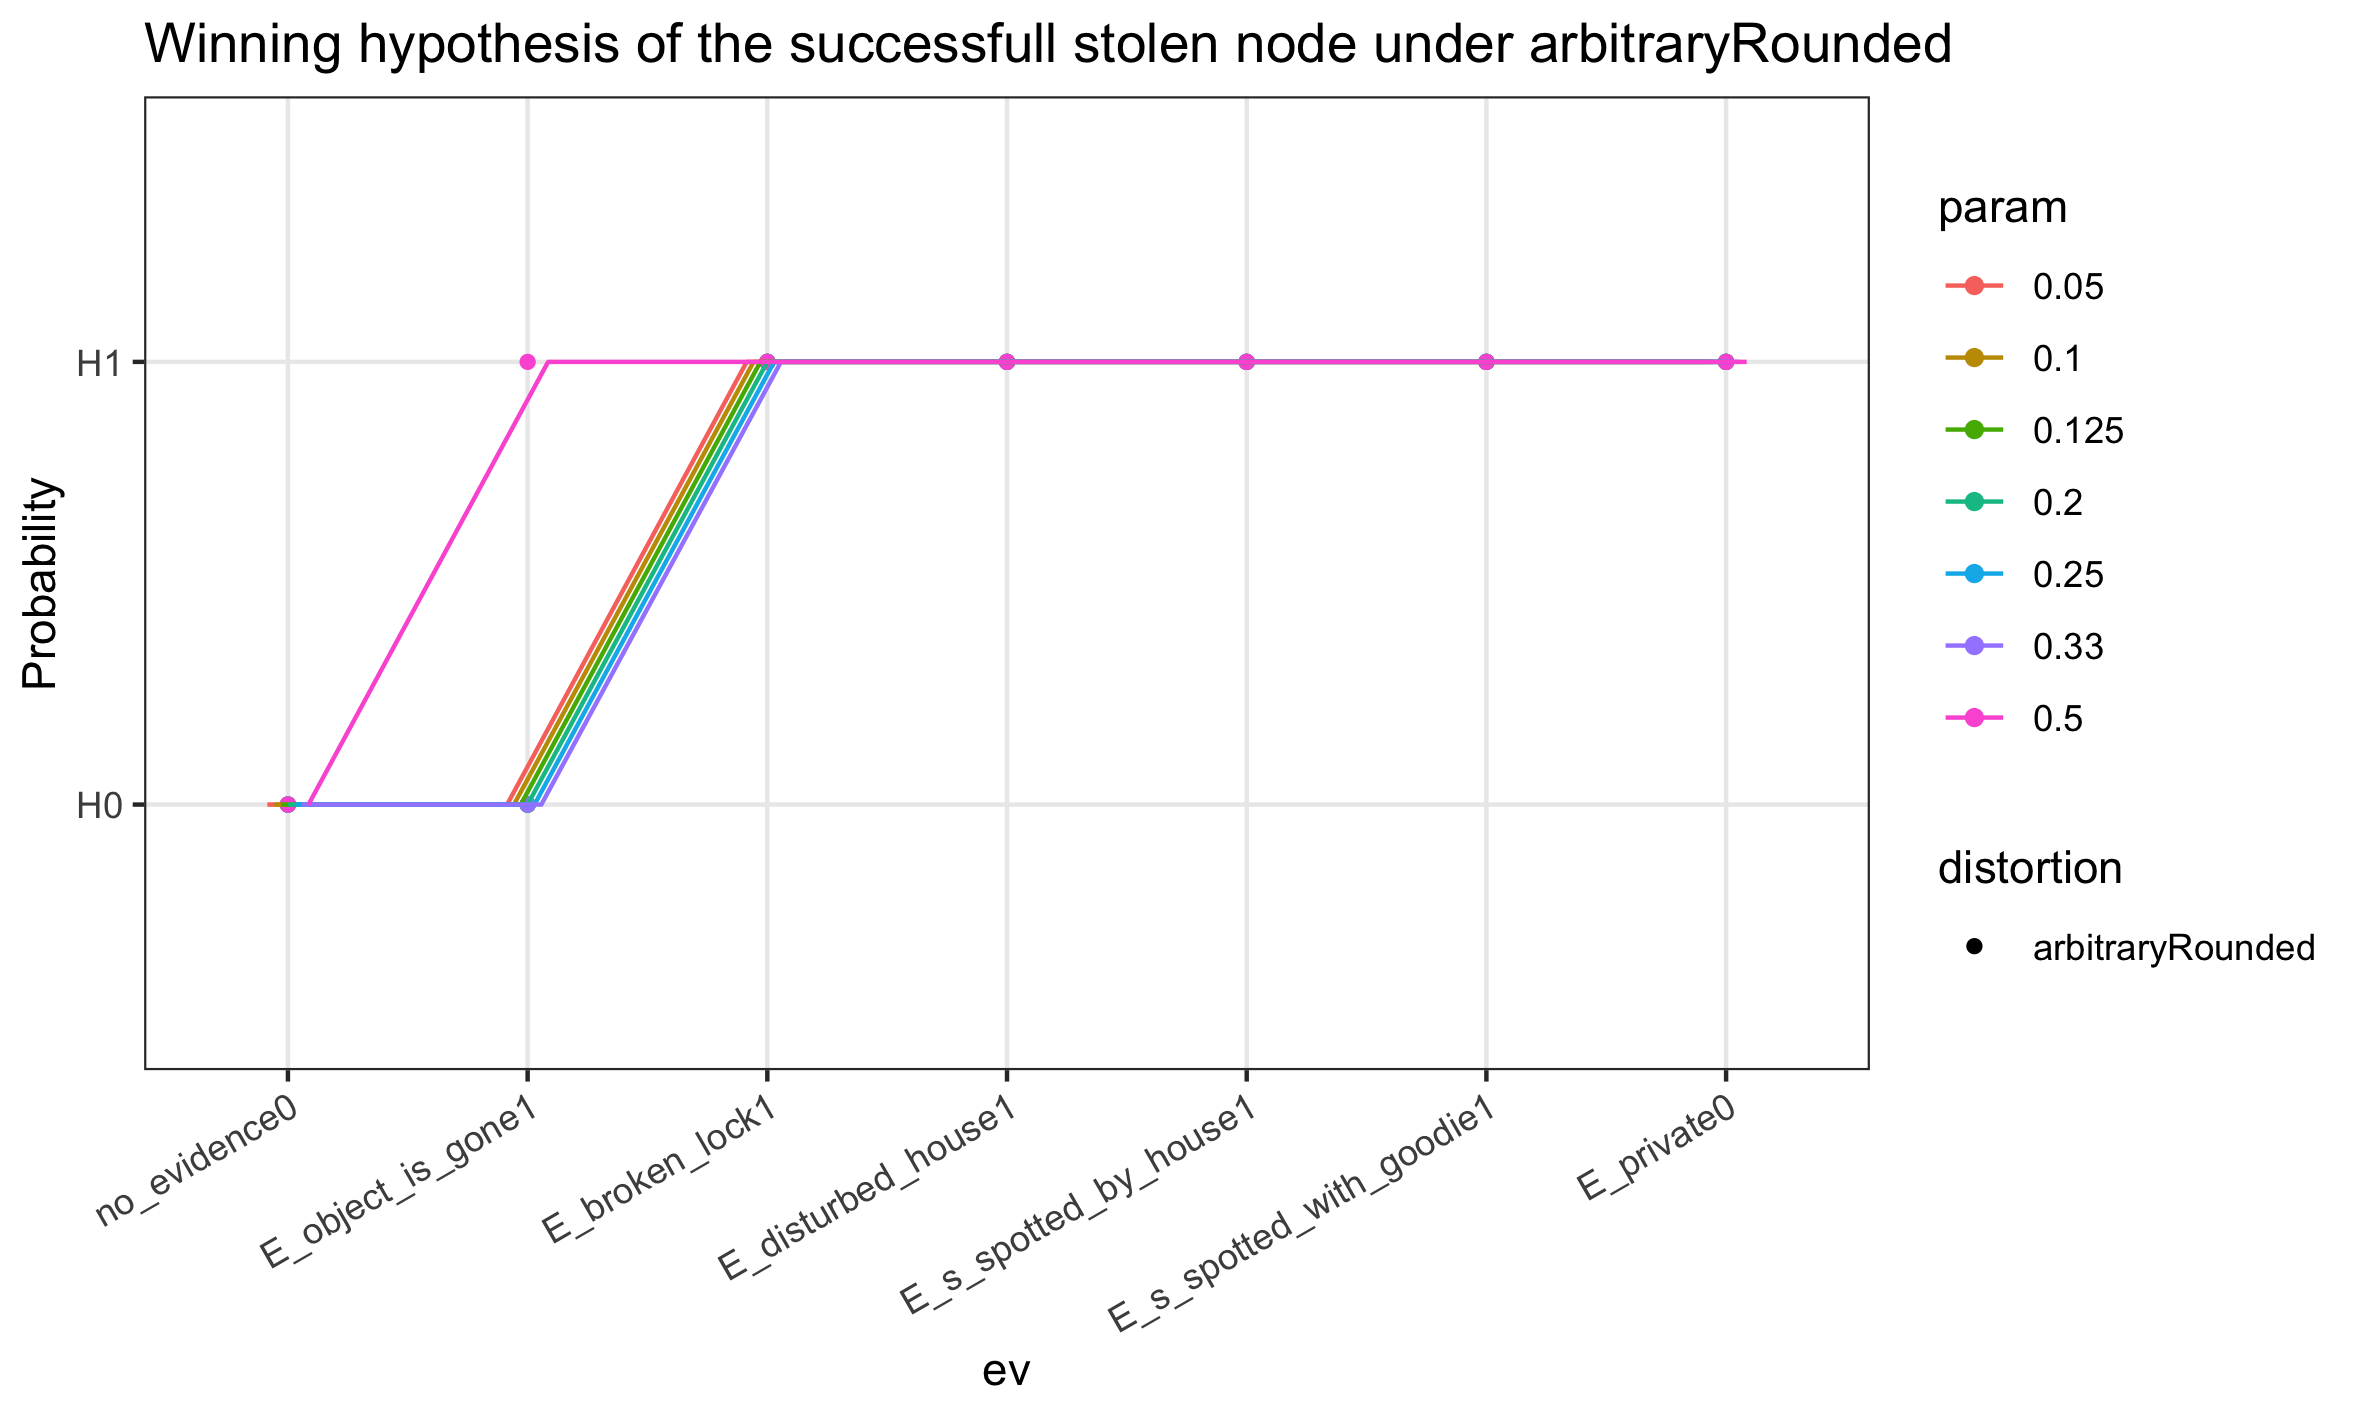
\includegraphics[scale=0.17]{images/arbitraryRoundedWeak.png}
\label{default}
\end{center}
\end{figure}
\begin{figure}[htbp]
\begin{center}
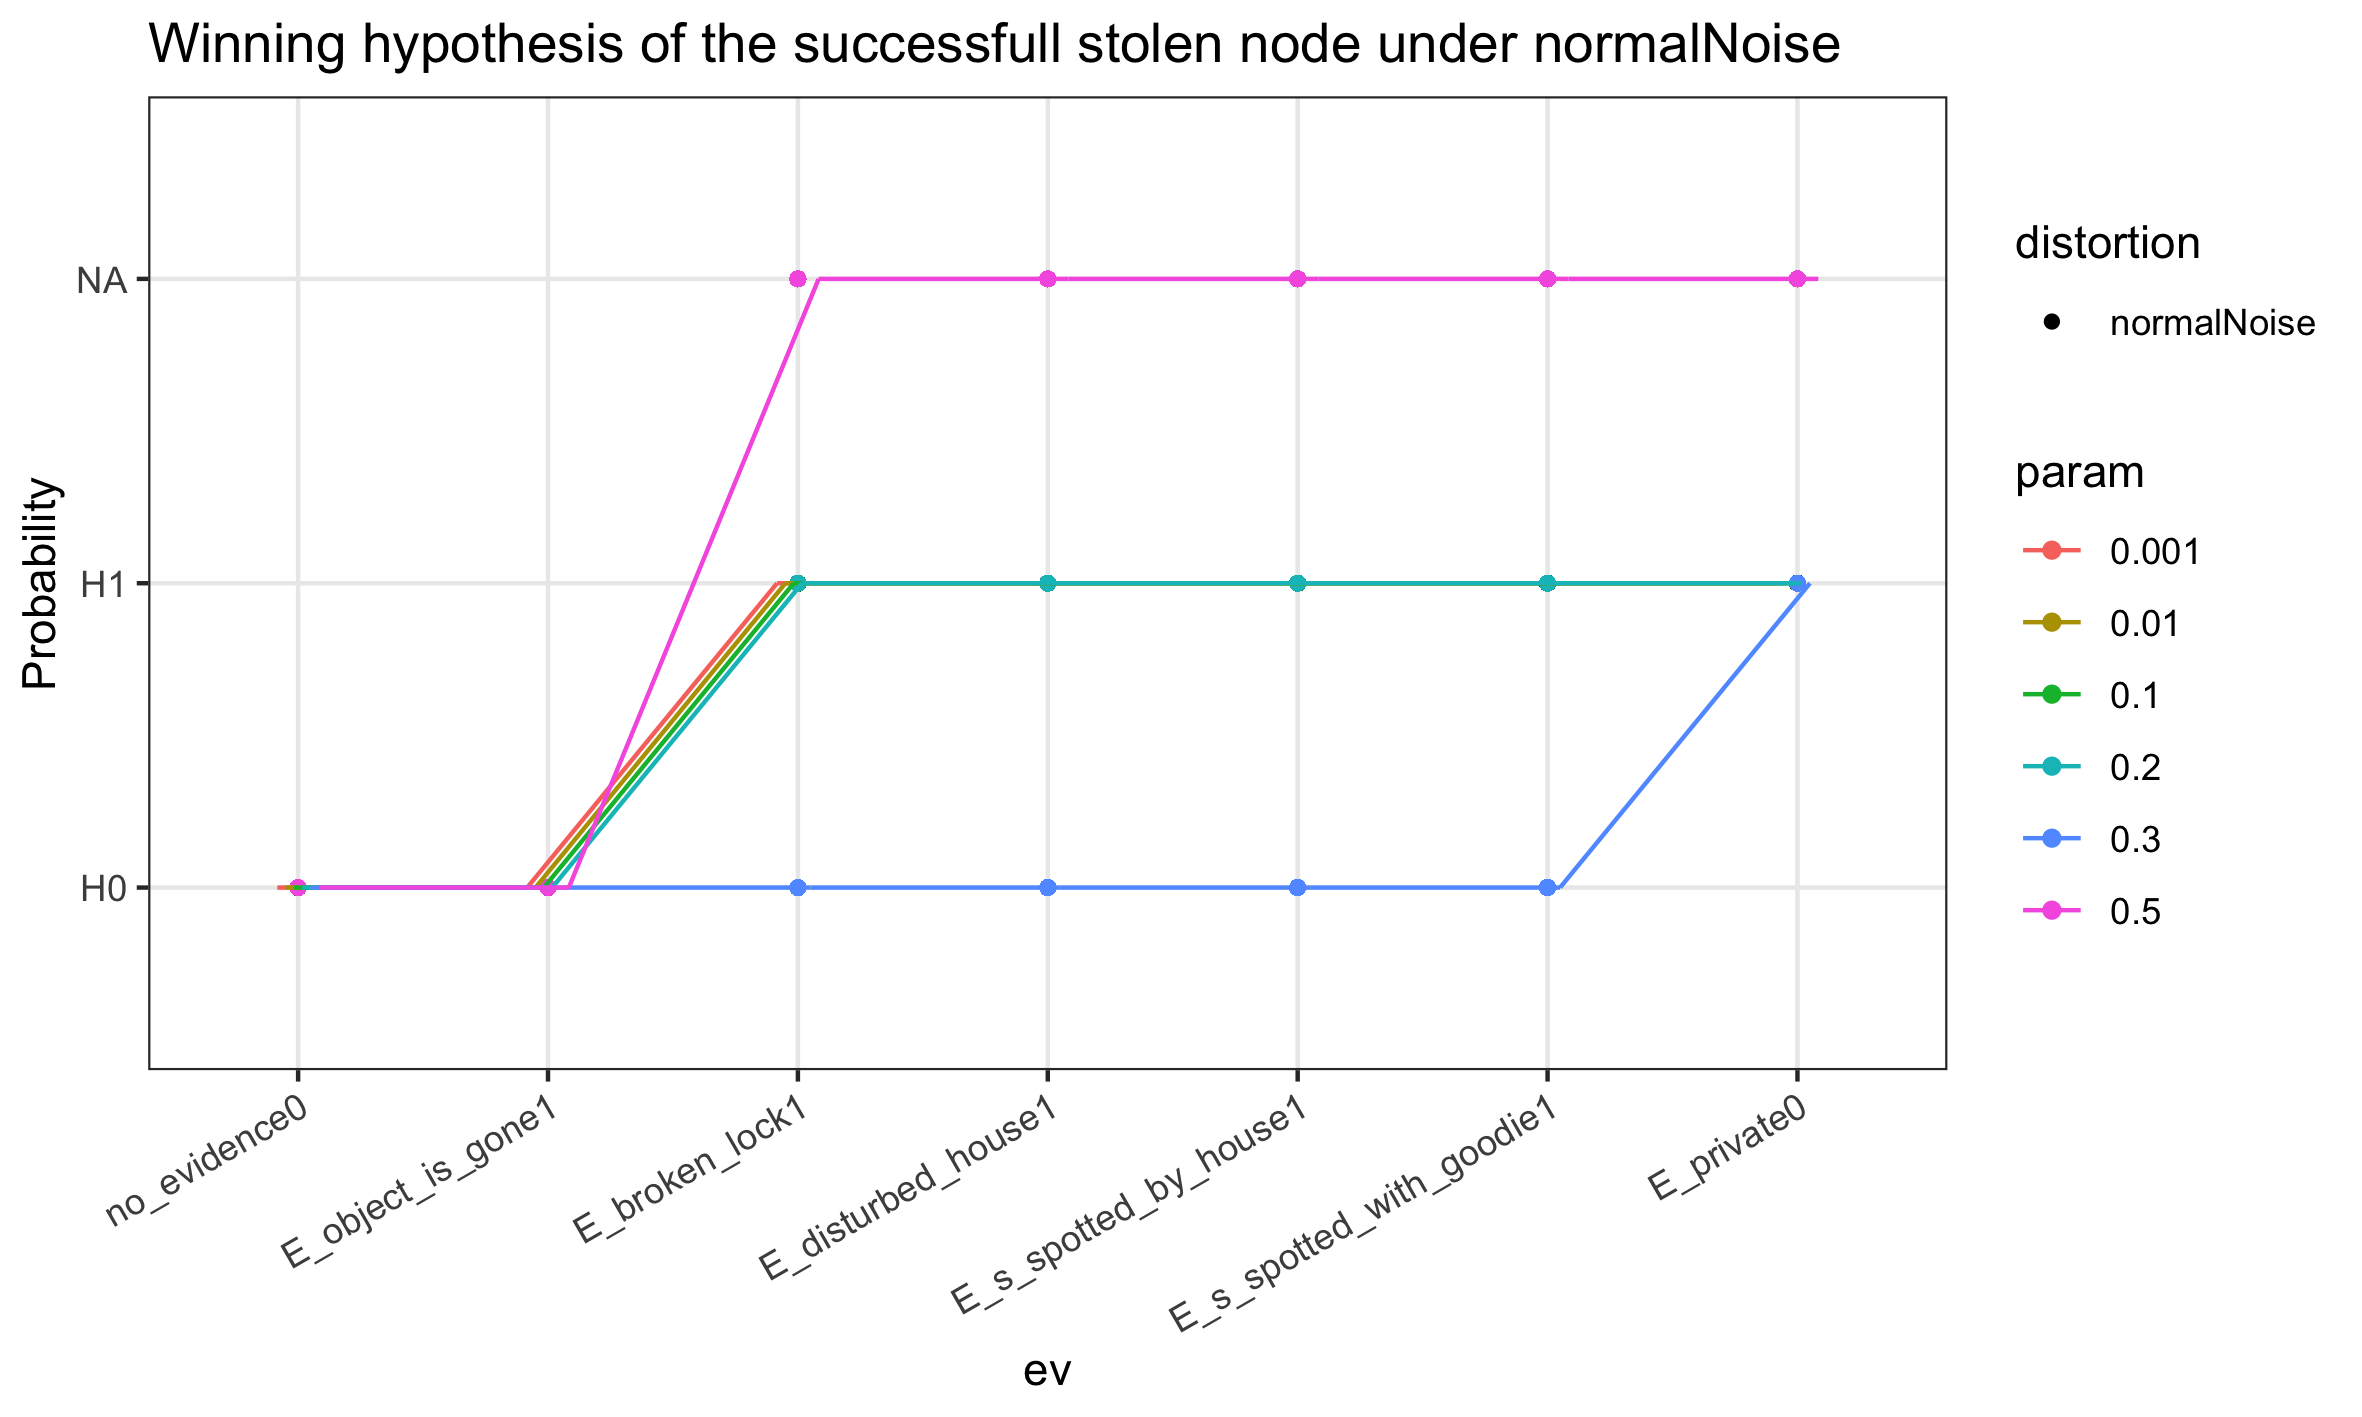
\includegraphics[scale=0.17]{images/normalNoiseWeak.png}
\label{default}
\end{center}
\end{figure}


\begin{figure}[htbp]
\centering
\begin{center}
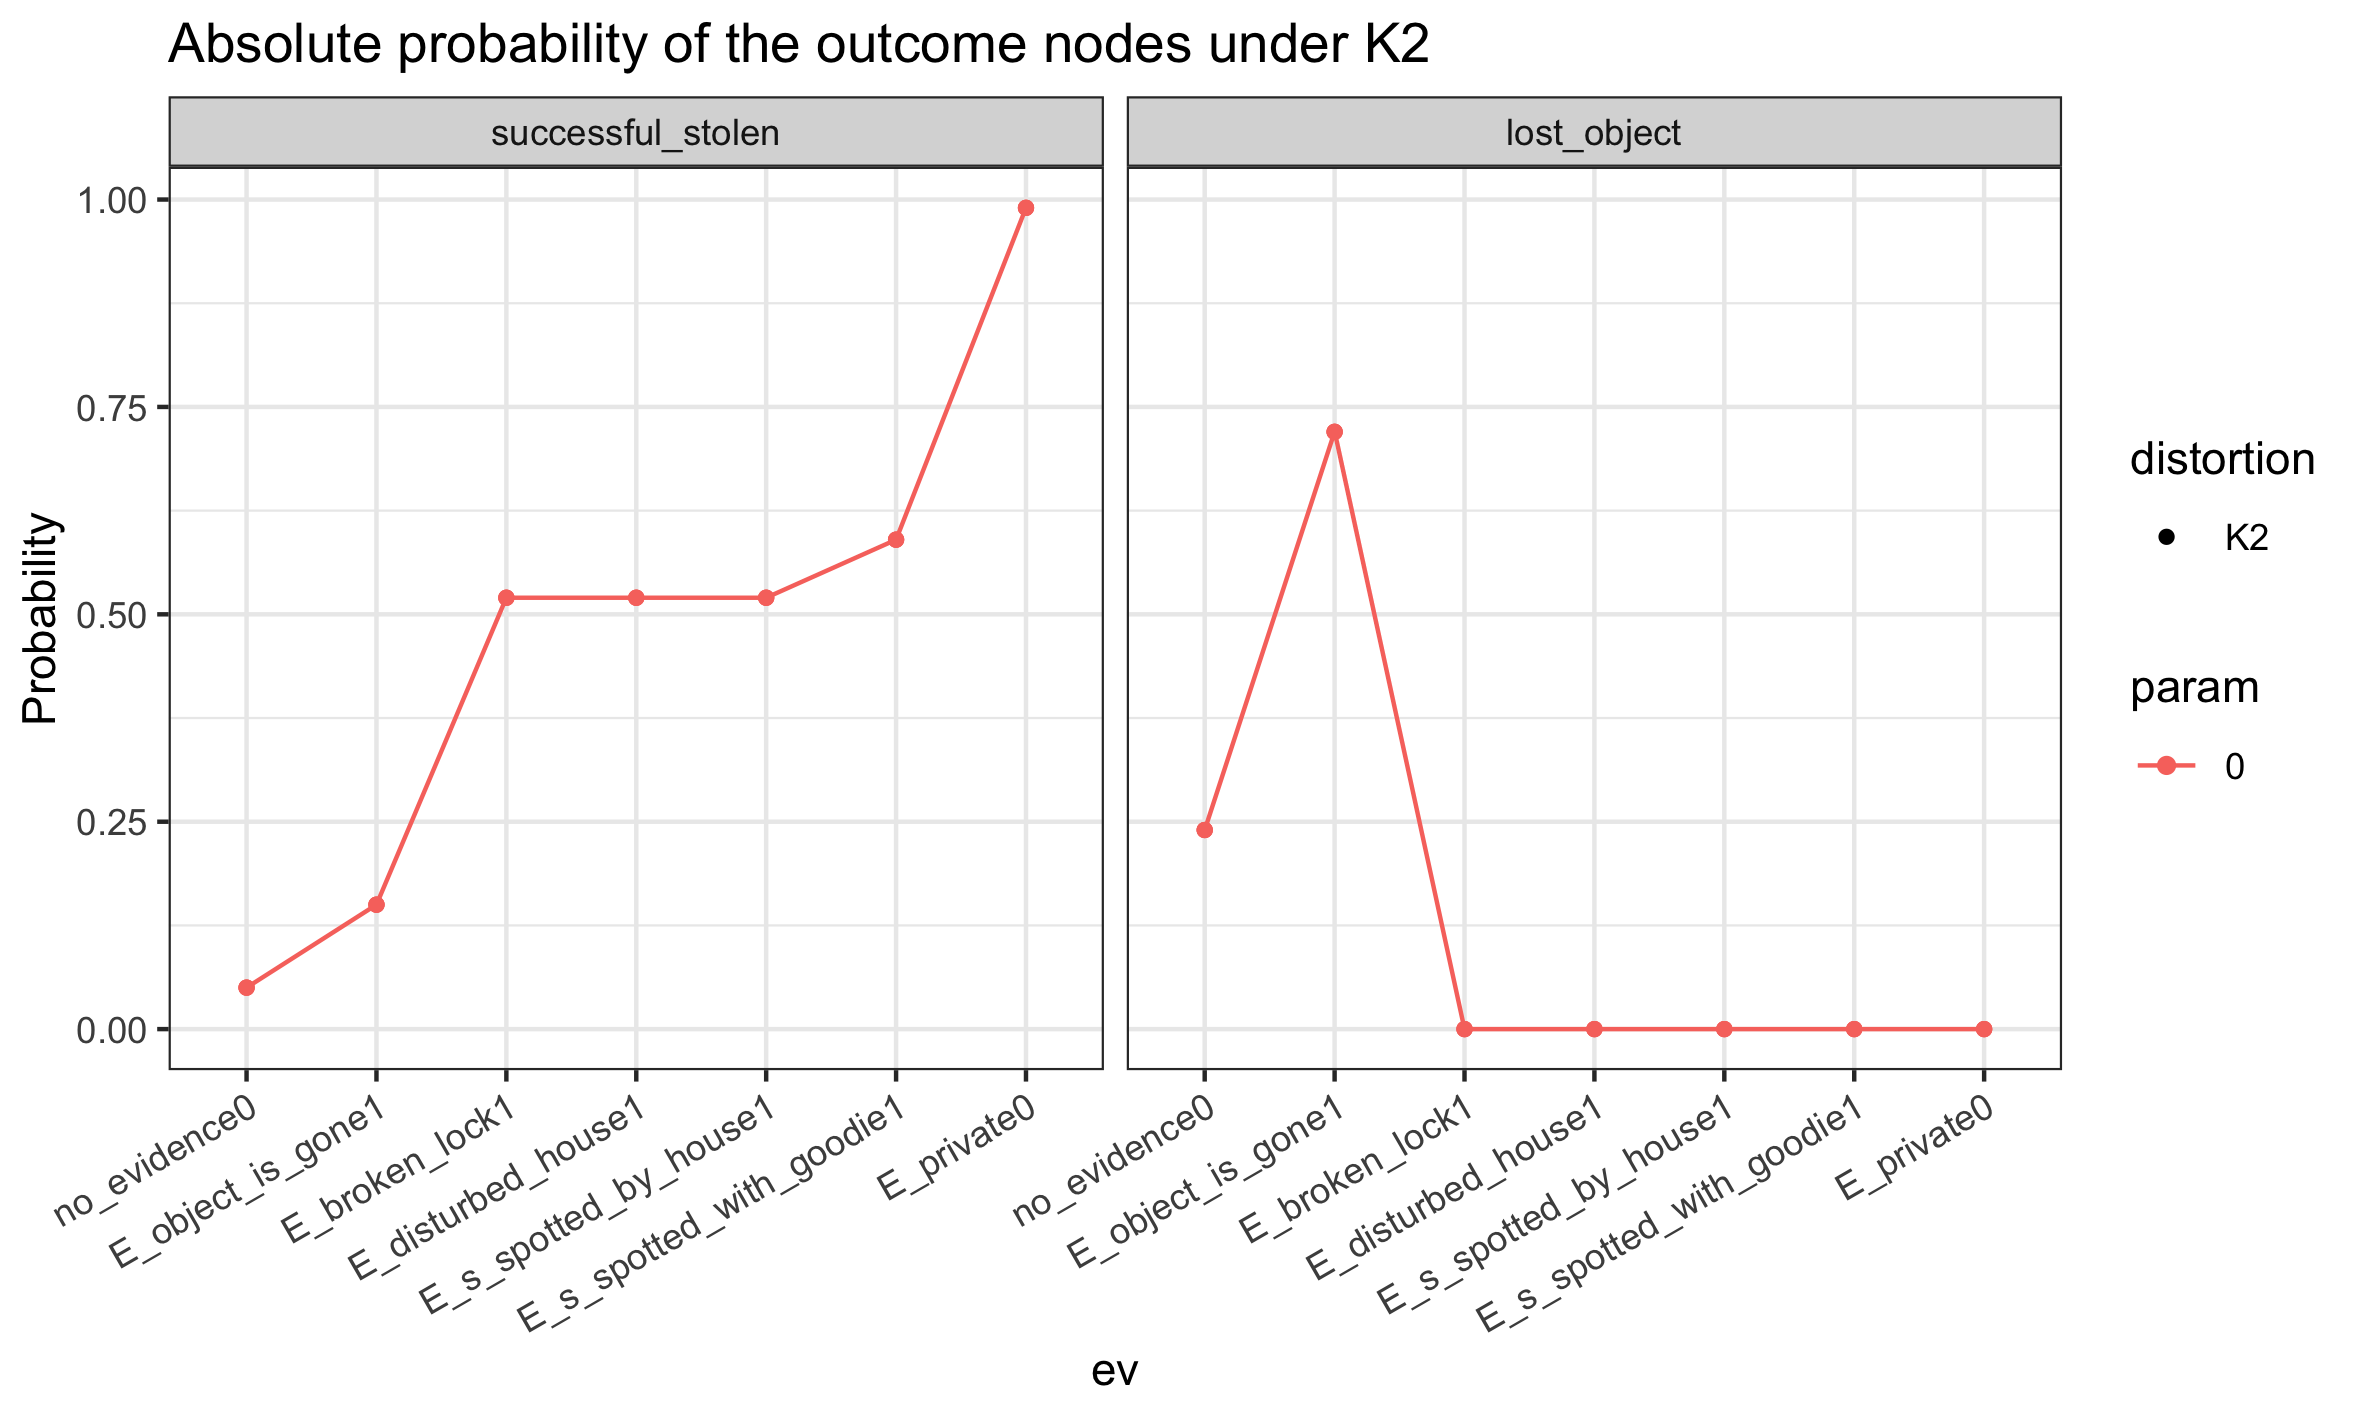
\includegraphics[scale=0.17]{images/K2absolute.png}
\label{default}
\end{center}
\end{figure}
\begin{figure}[htbp]
\centering
\begin{center}
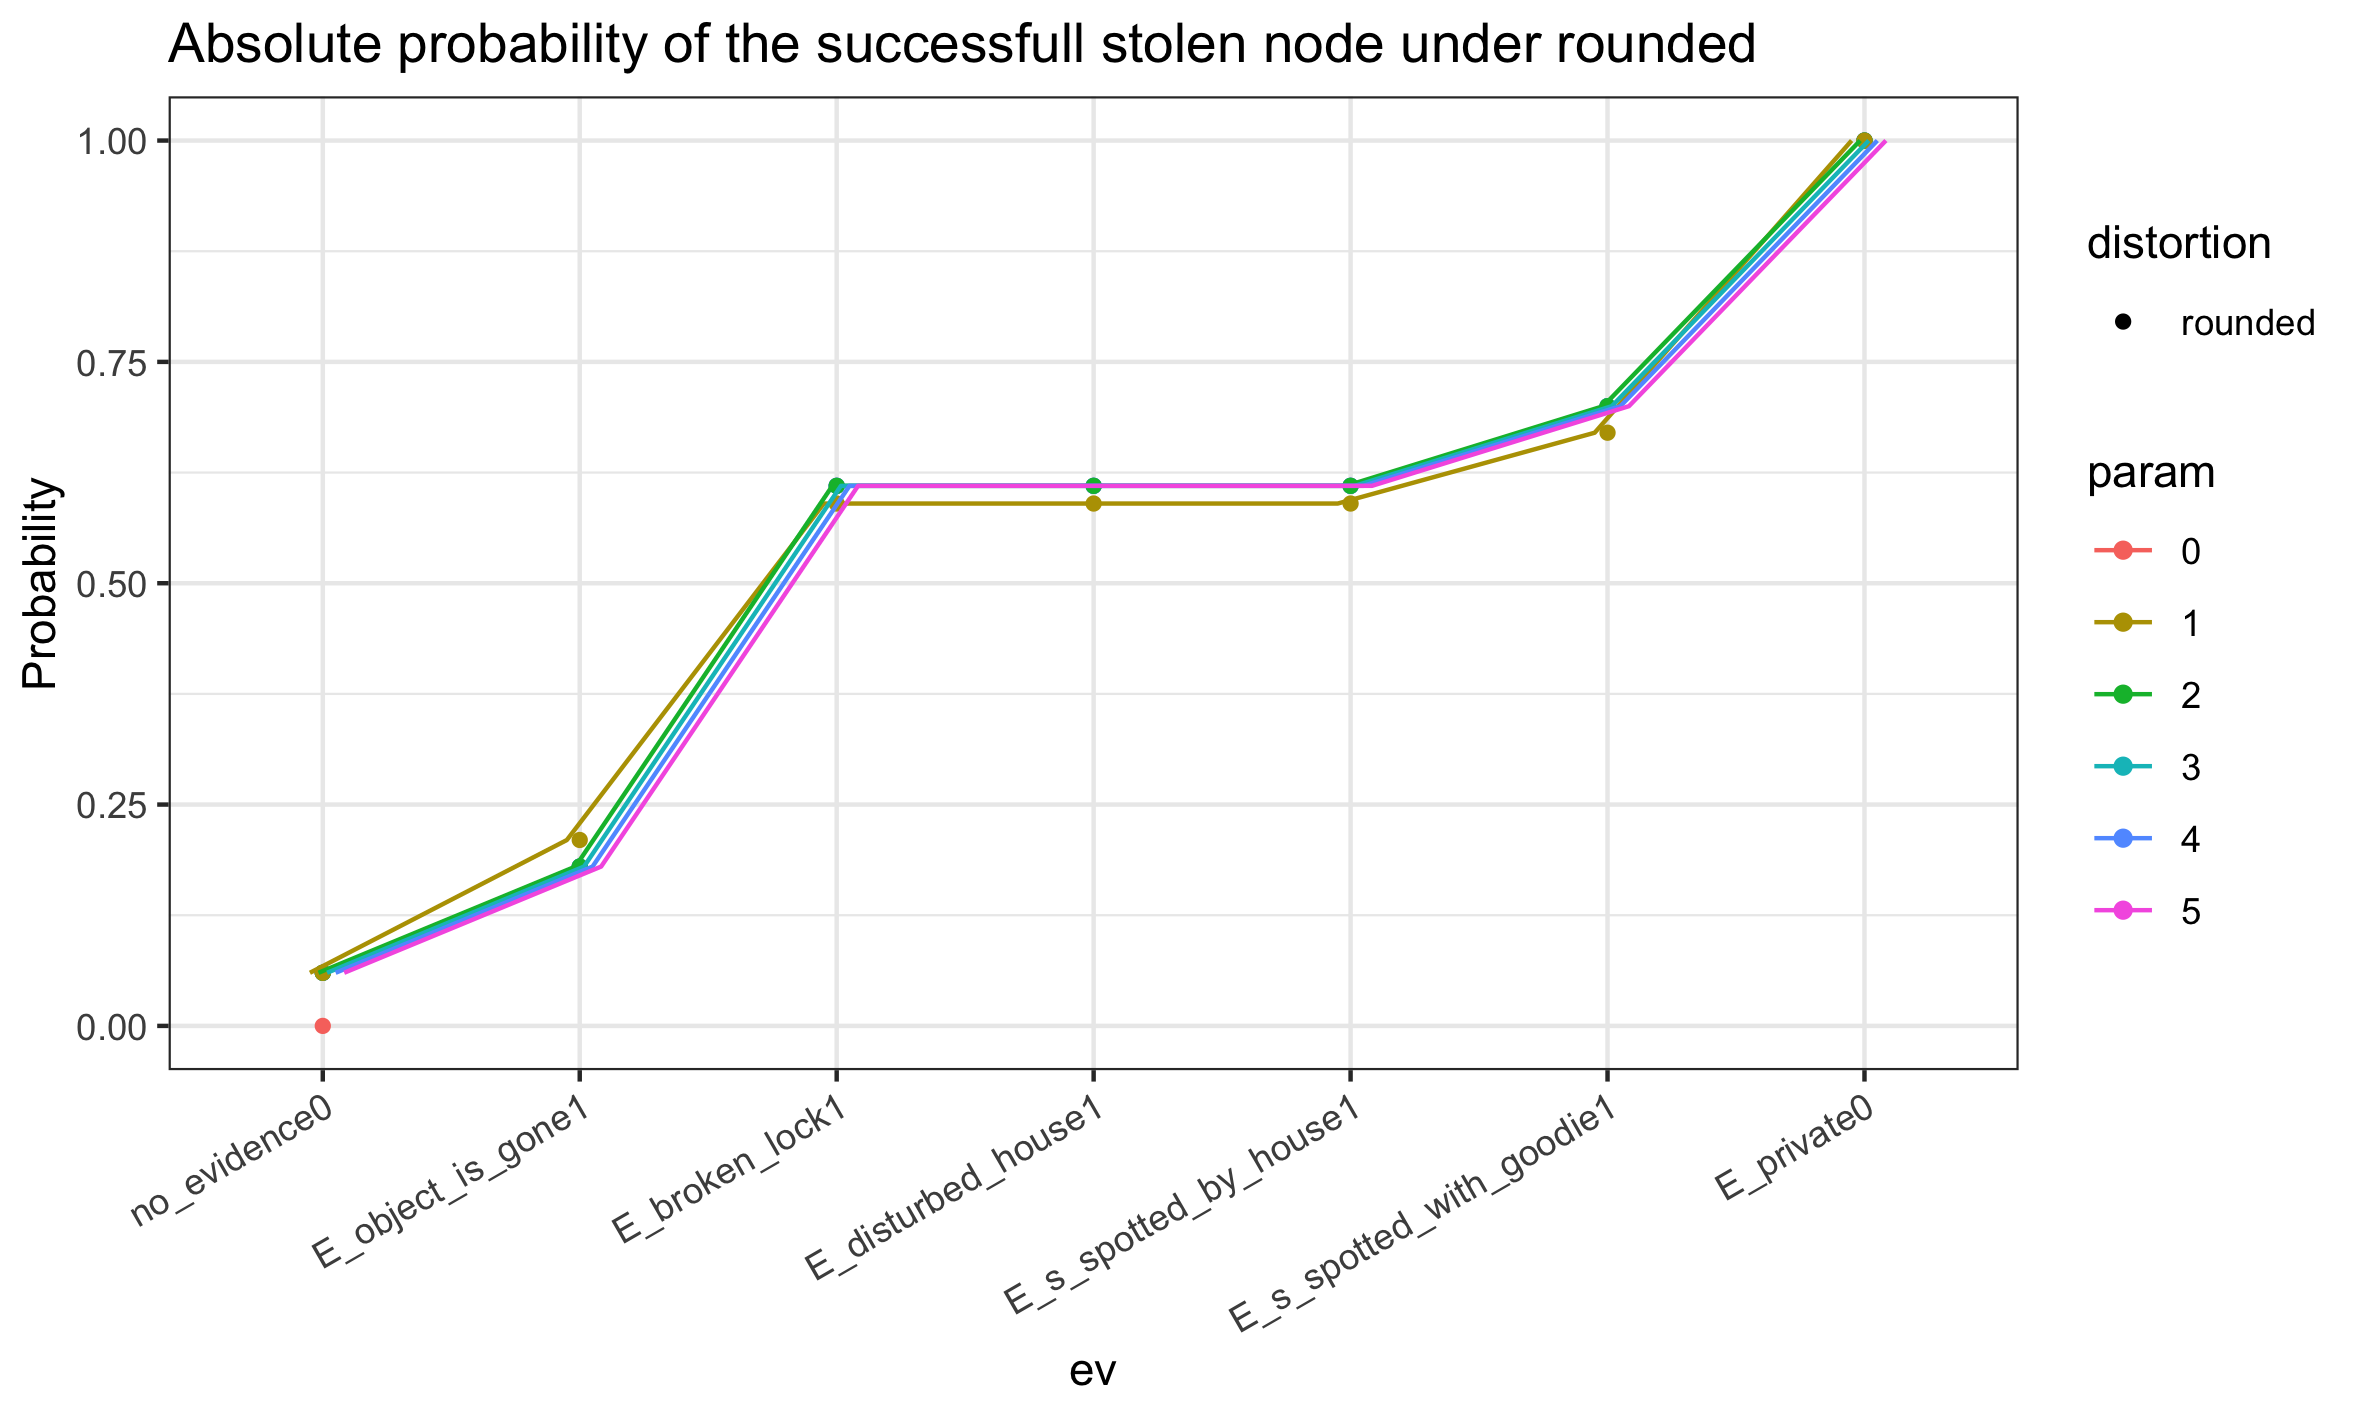
\includegraphics[scale=0.17]{images/roundedabsolute.png}
\label{default}
\end{center}
\end{figure}
\begin{figure}[htbp]
\centering
\begin{center}
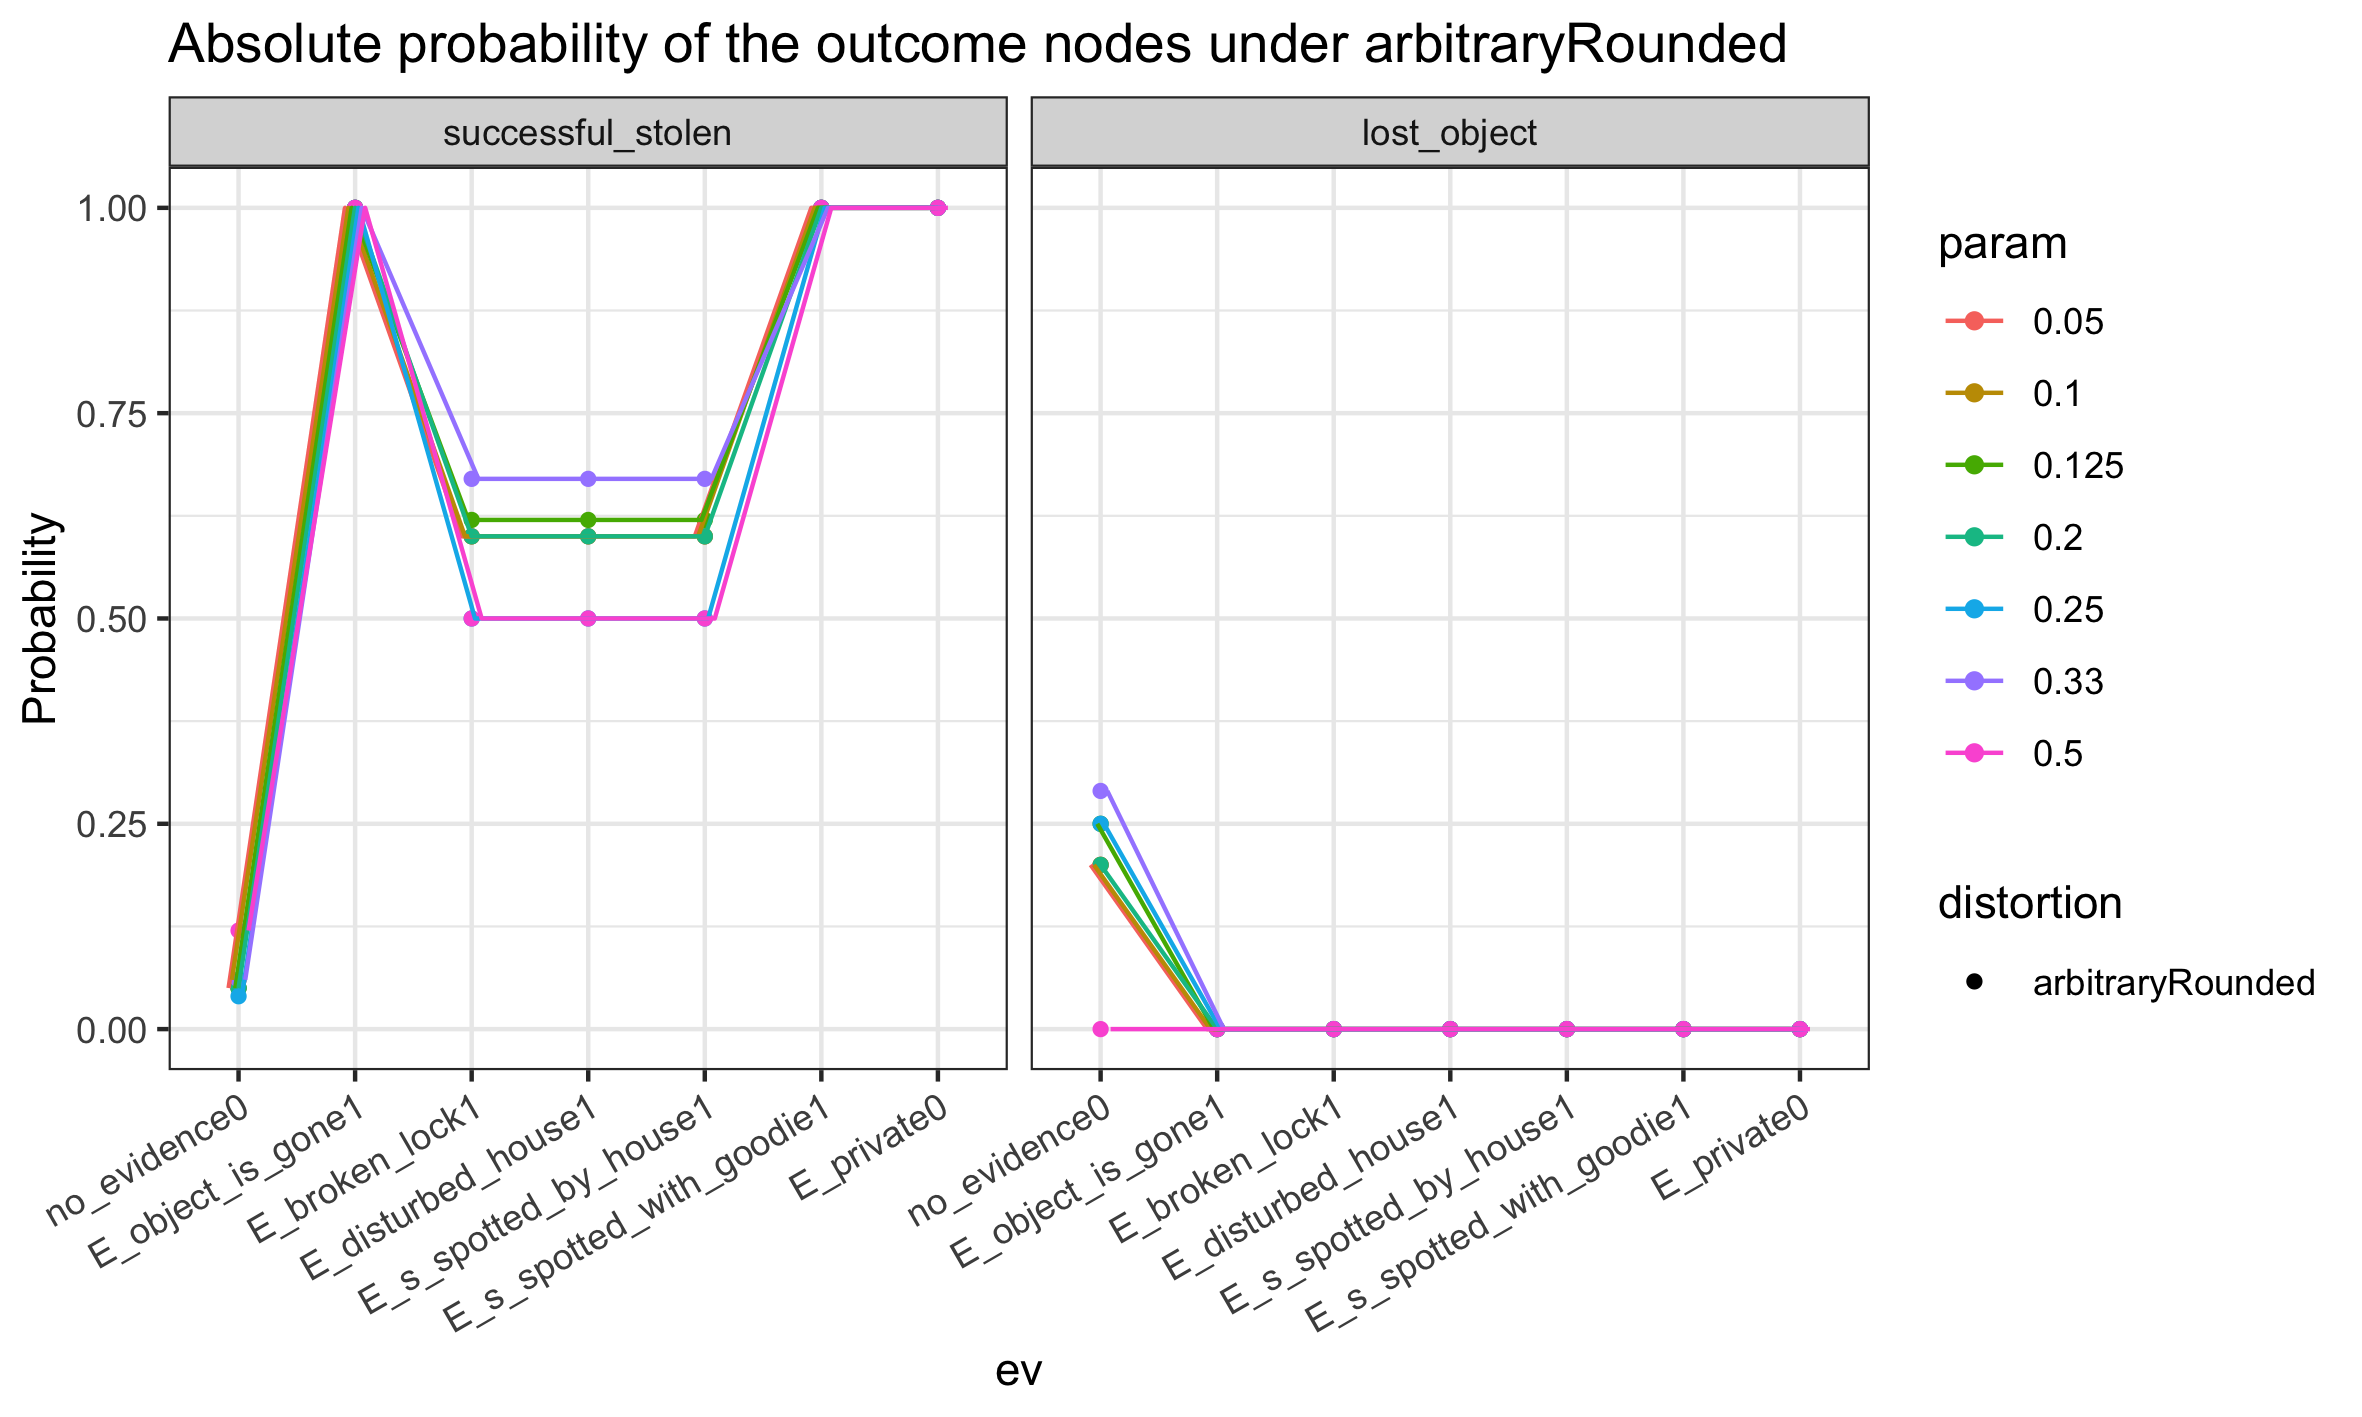
\includegraphics[scale=0.17]{images/arbitraryRoundedabsolute.png}
\label{default}
\end{center}
\end{figure}
\begin{figure}[htbp]
\centering
\begin{center}
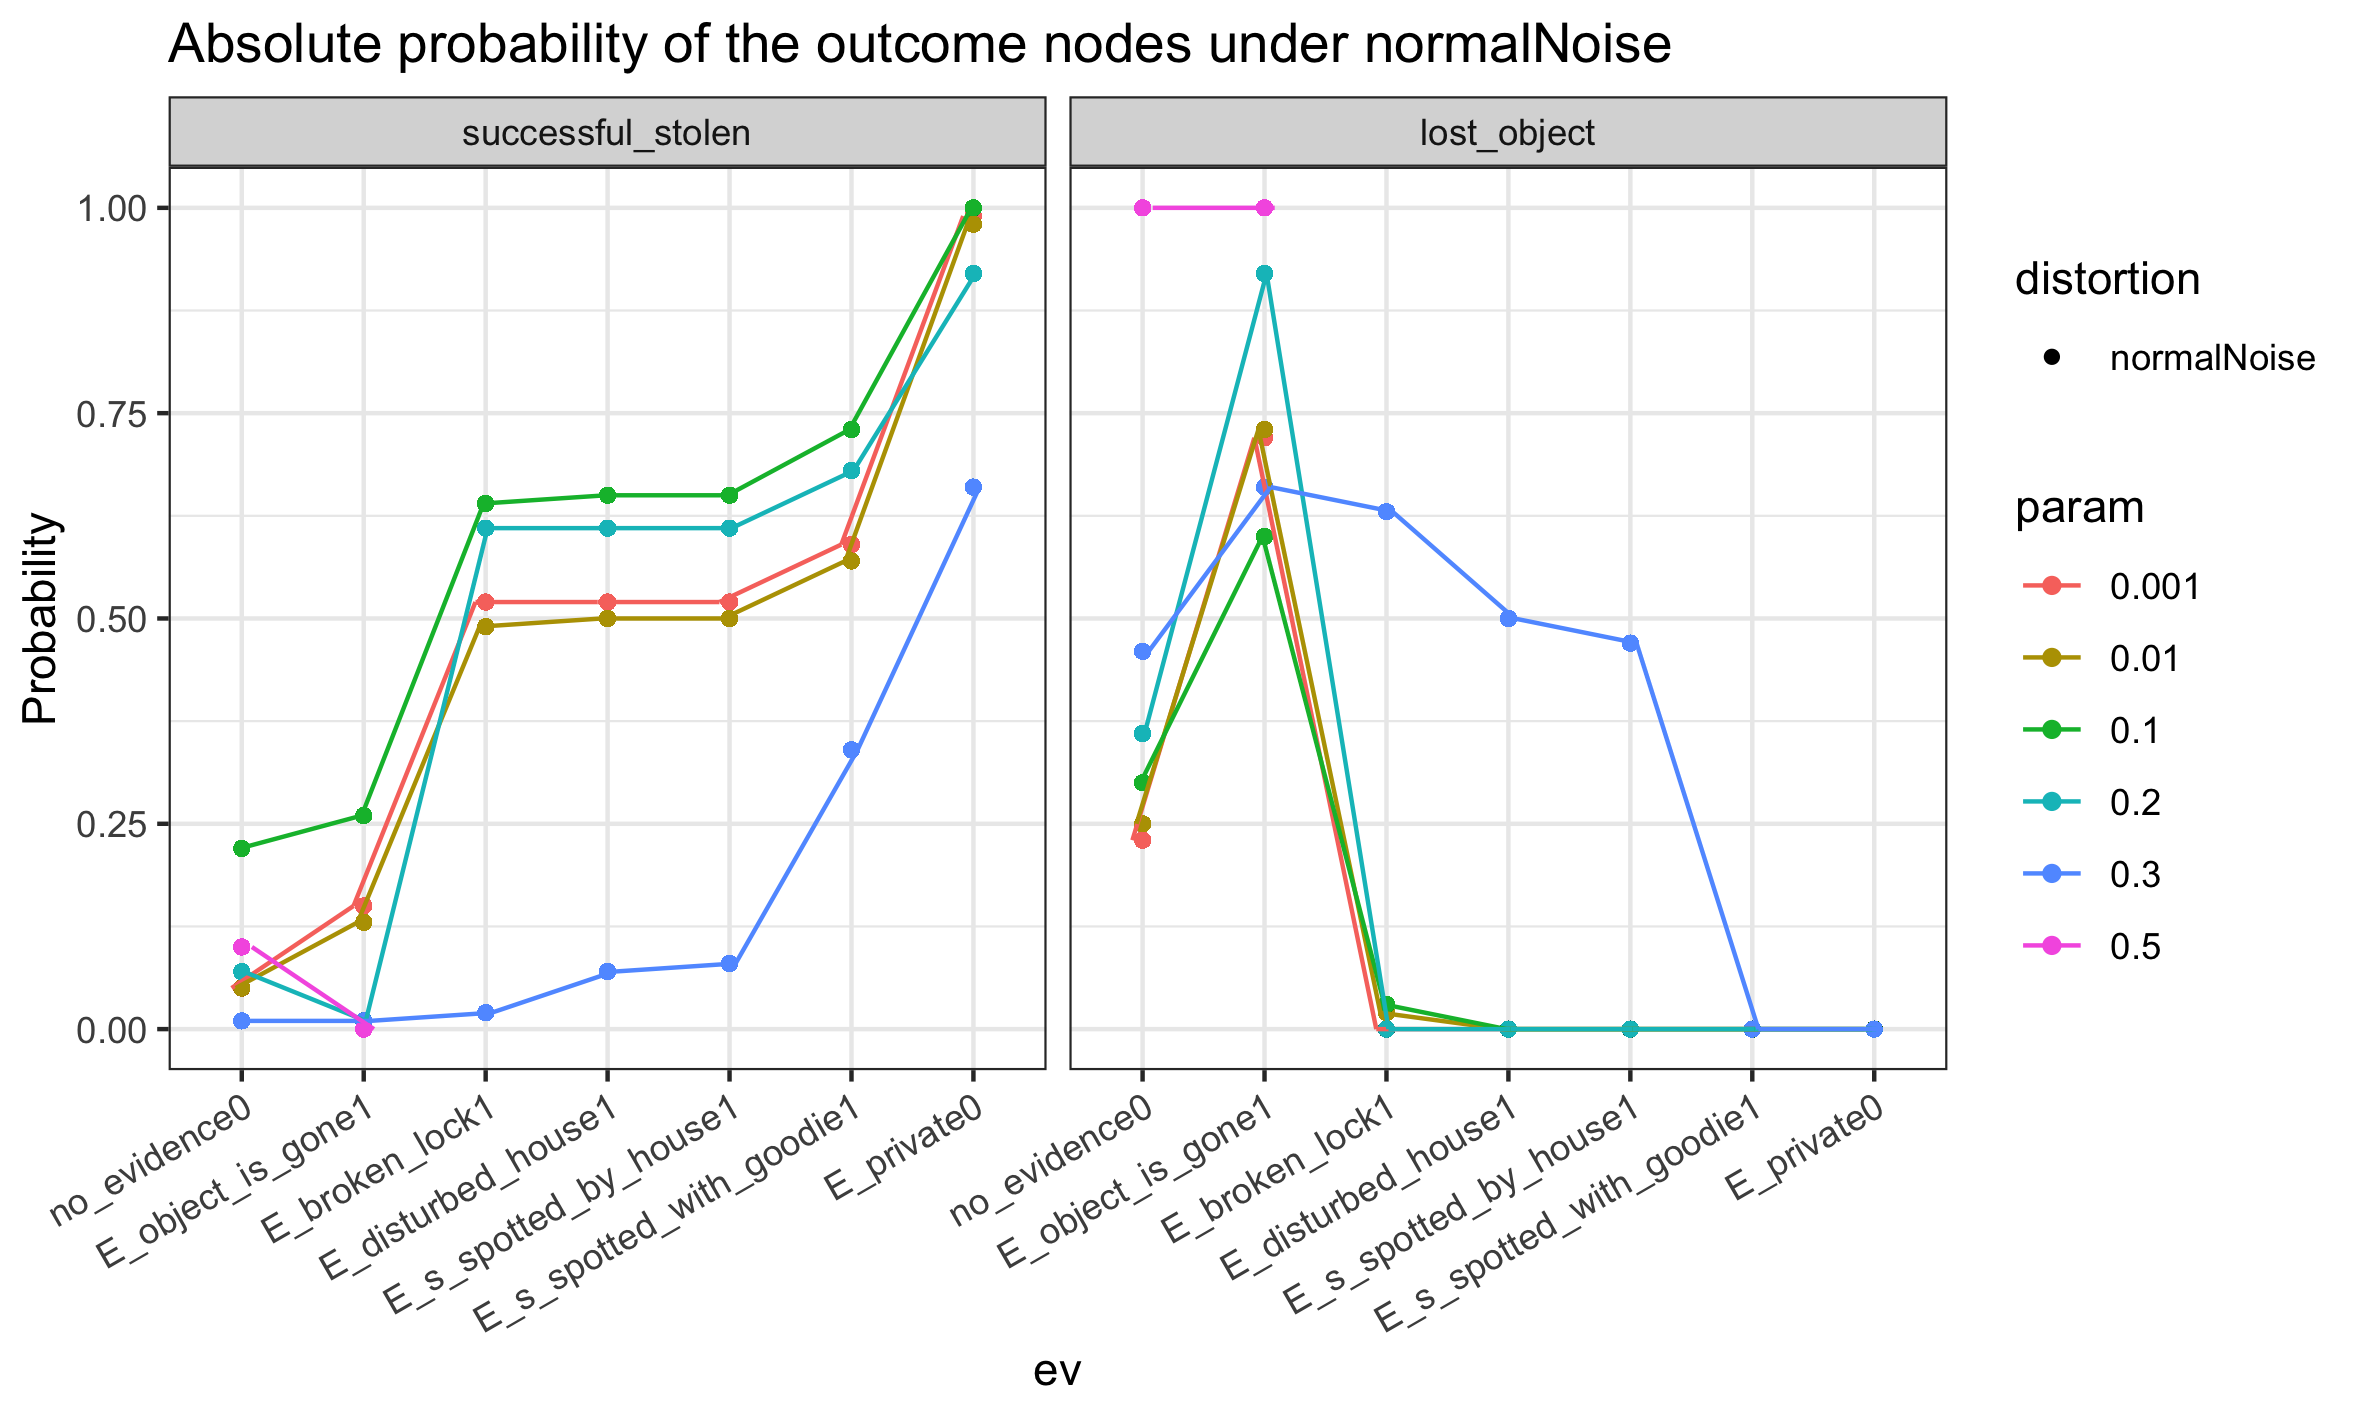
\includegraphics[scale=0.17]{images/normalNoiseabsolute.png}
\label{default}
\end{center}
\end{figure}



\begin{figure}[htbp]
\begin{center}
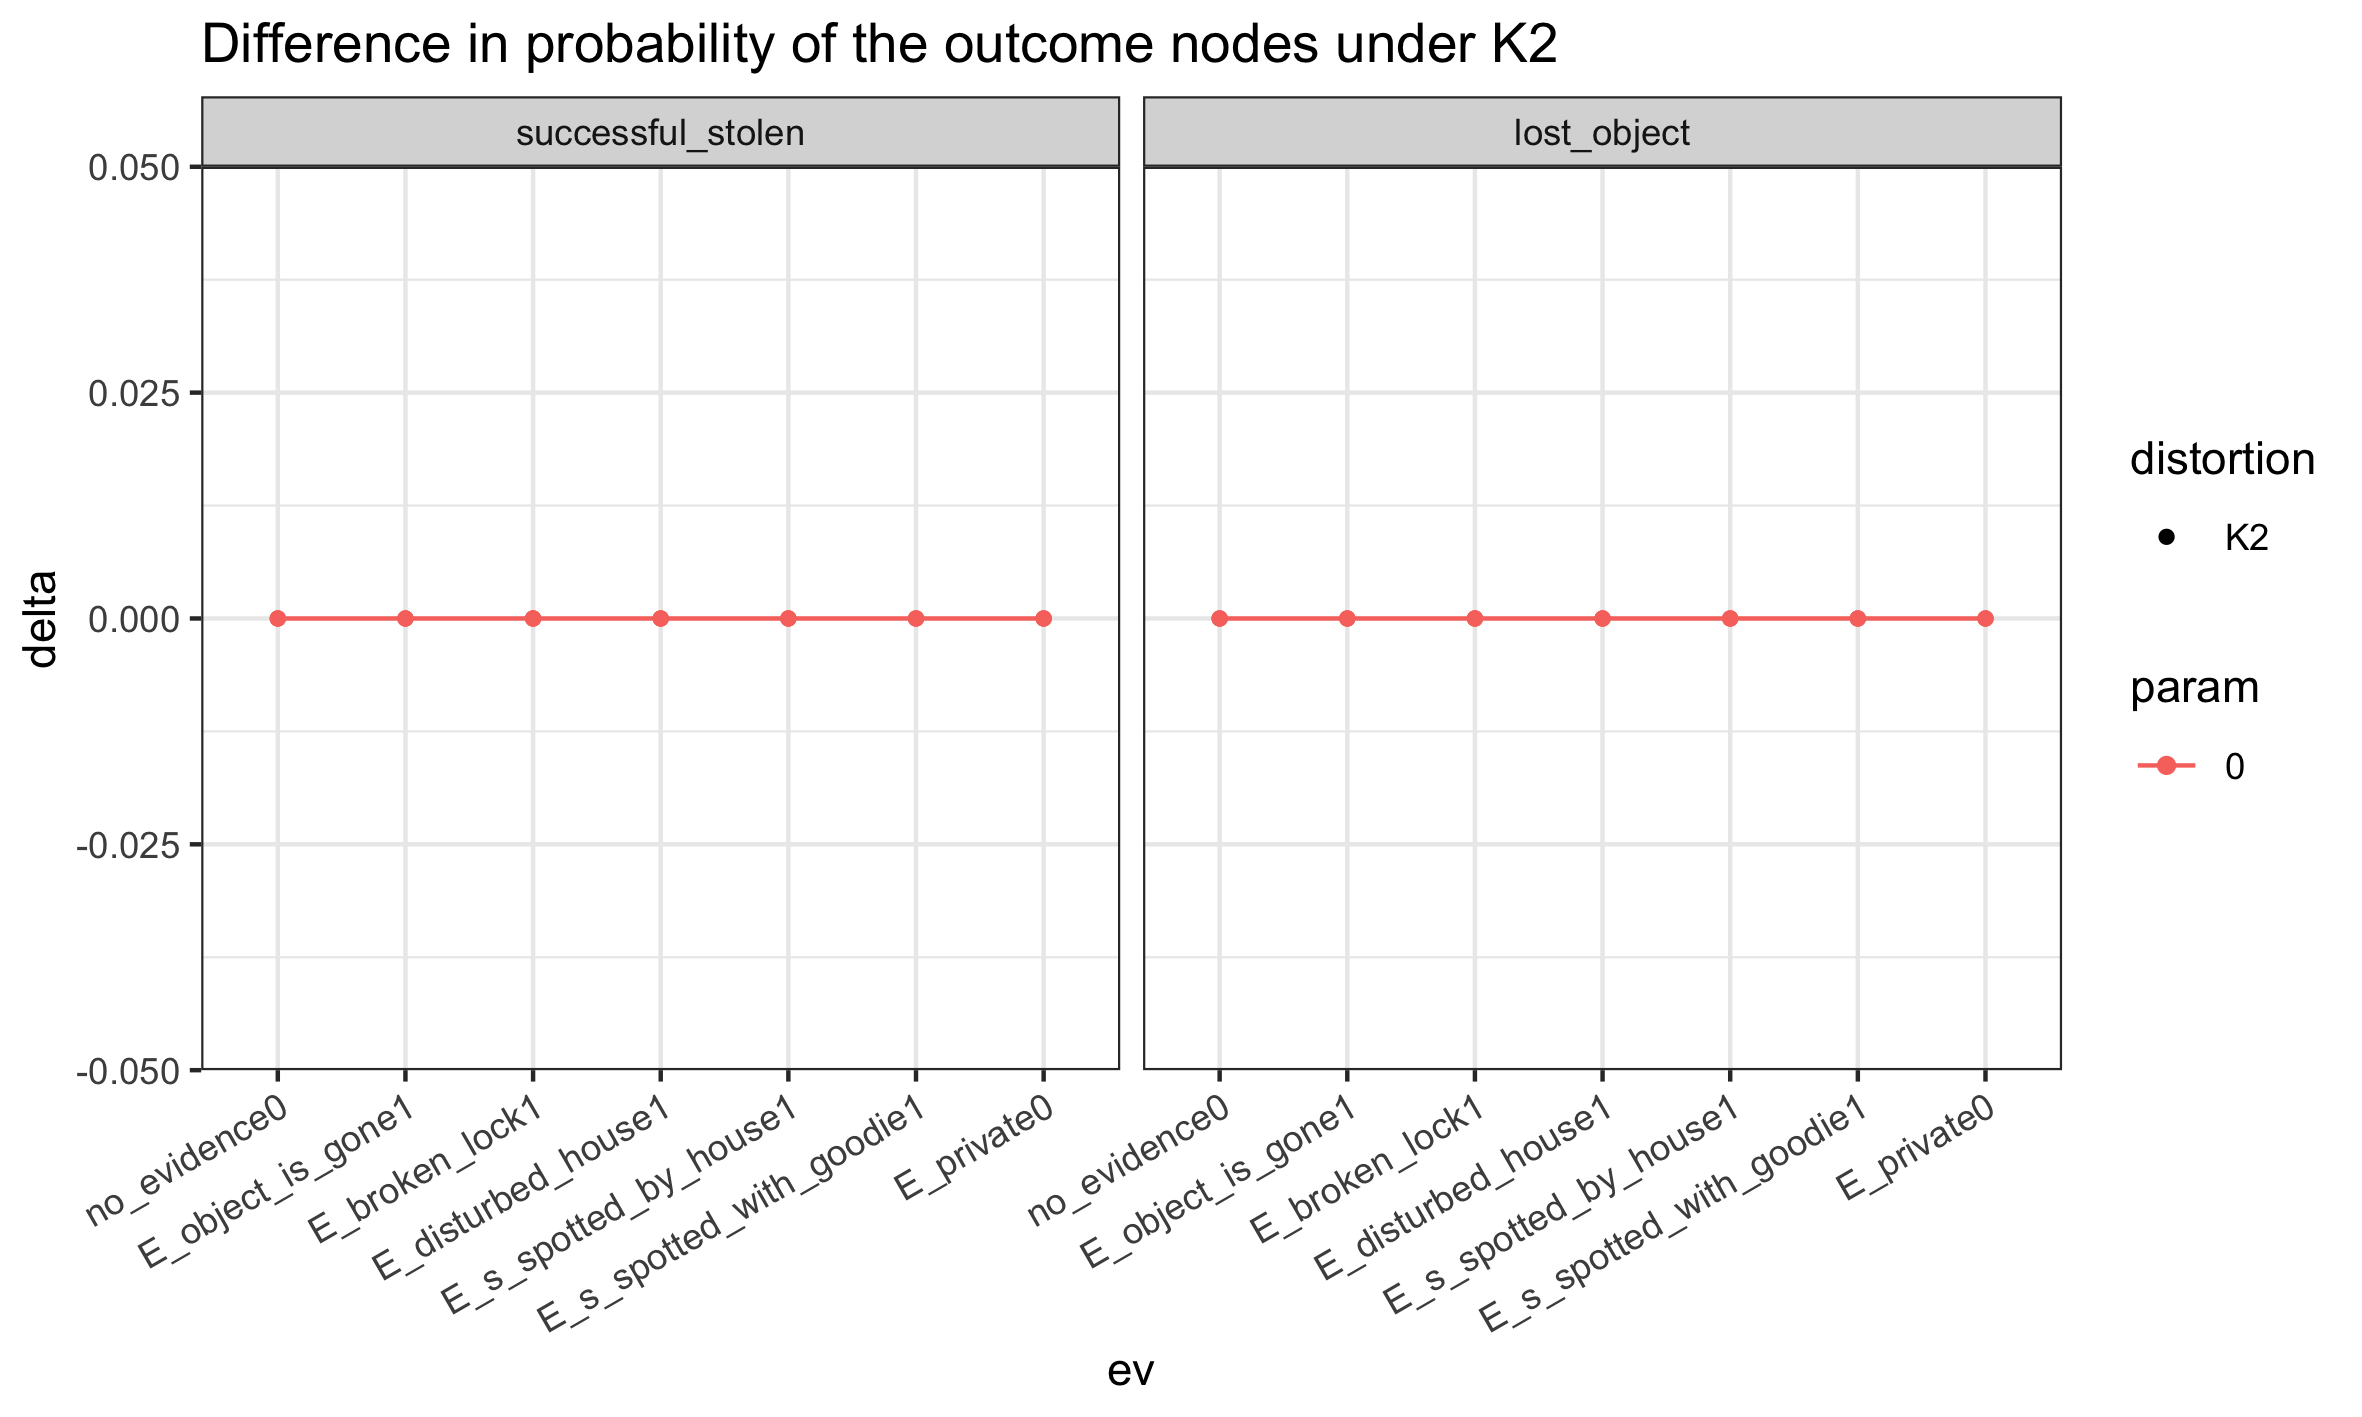
\includegraphics[scale=0.17]{images/K2delta.png}
\label{default}
\end{center}
\end{figure}

\begin{figure}[htbp]
\begin{center}
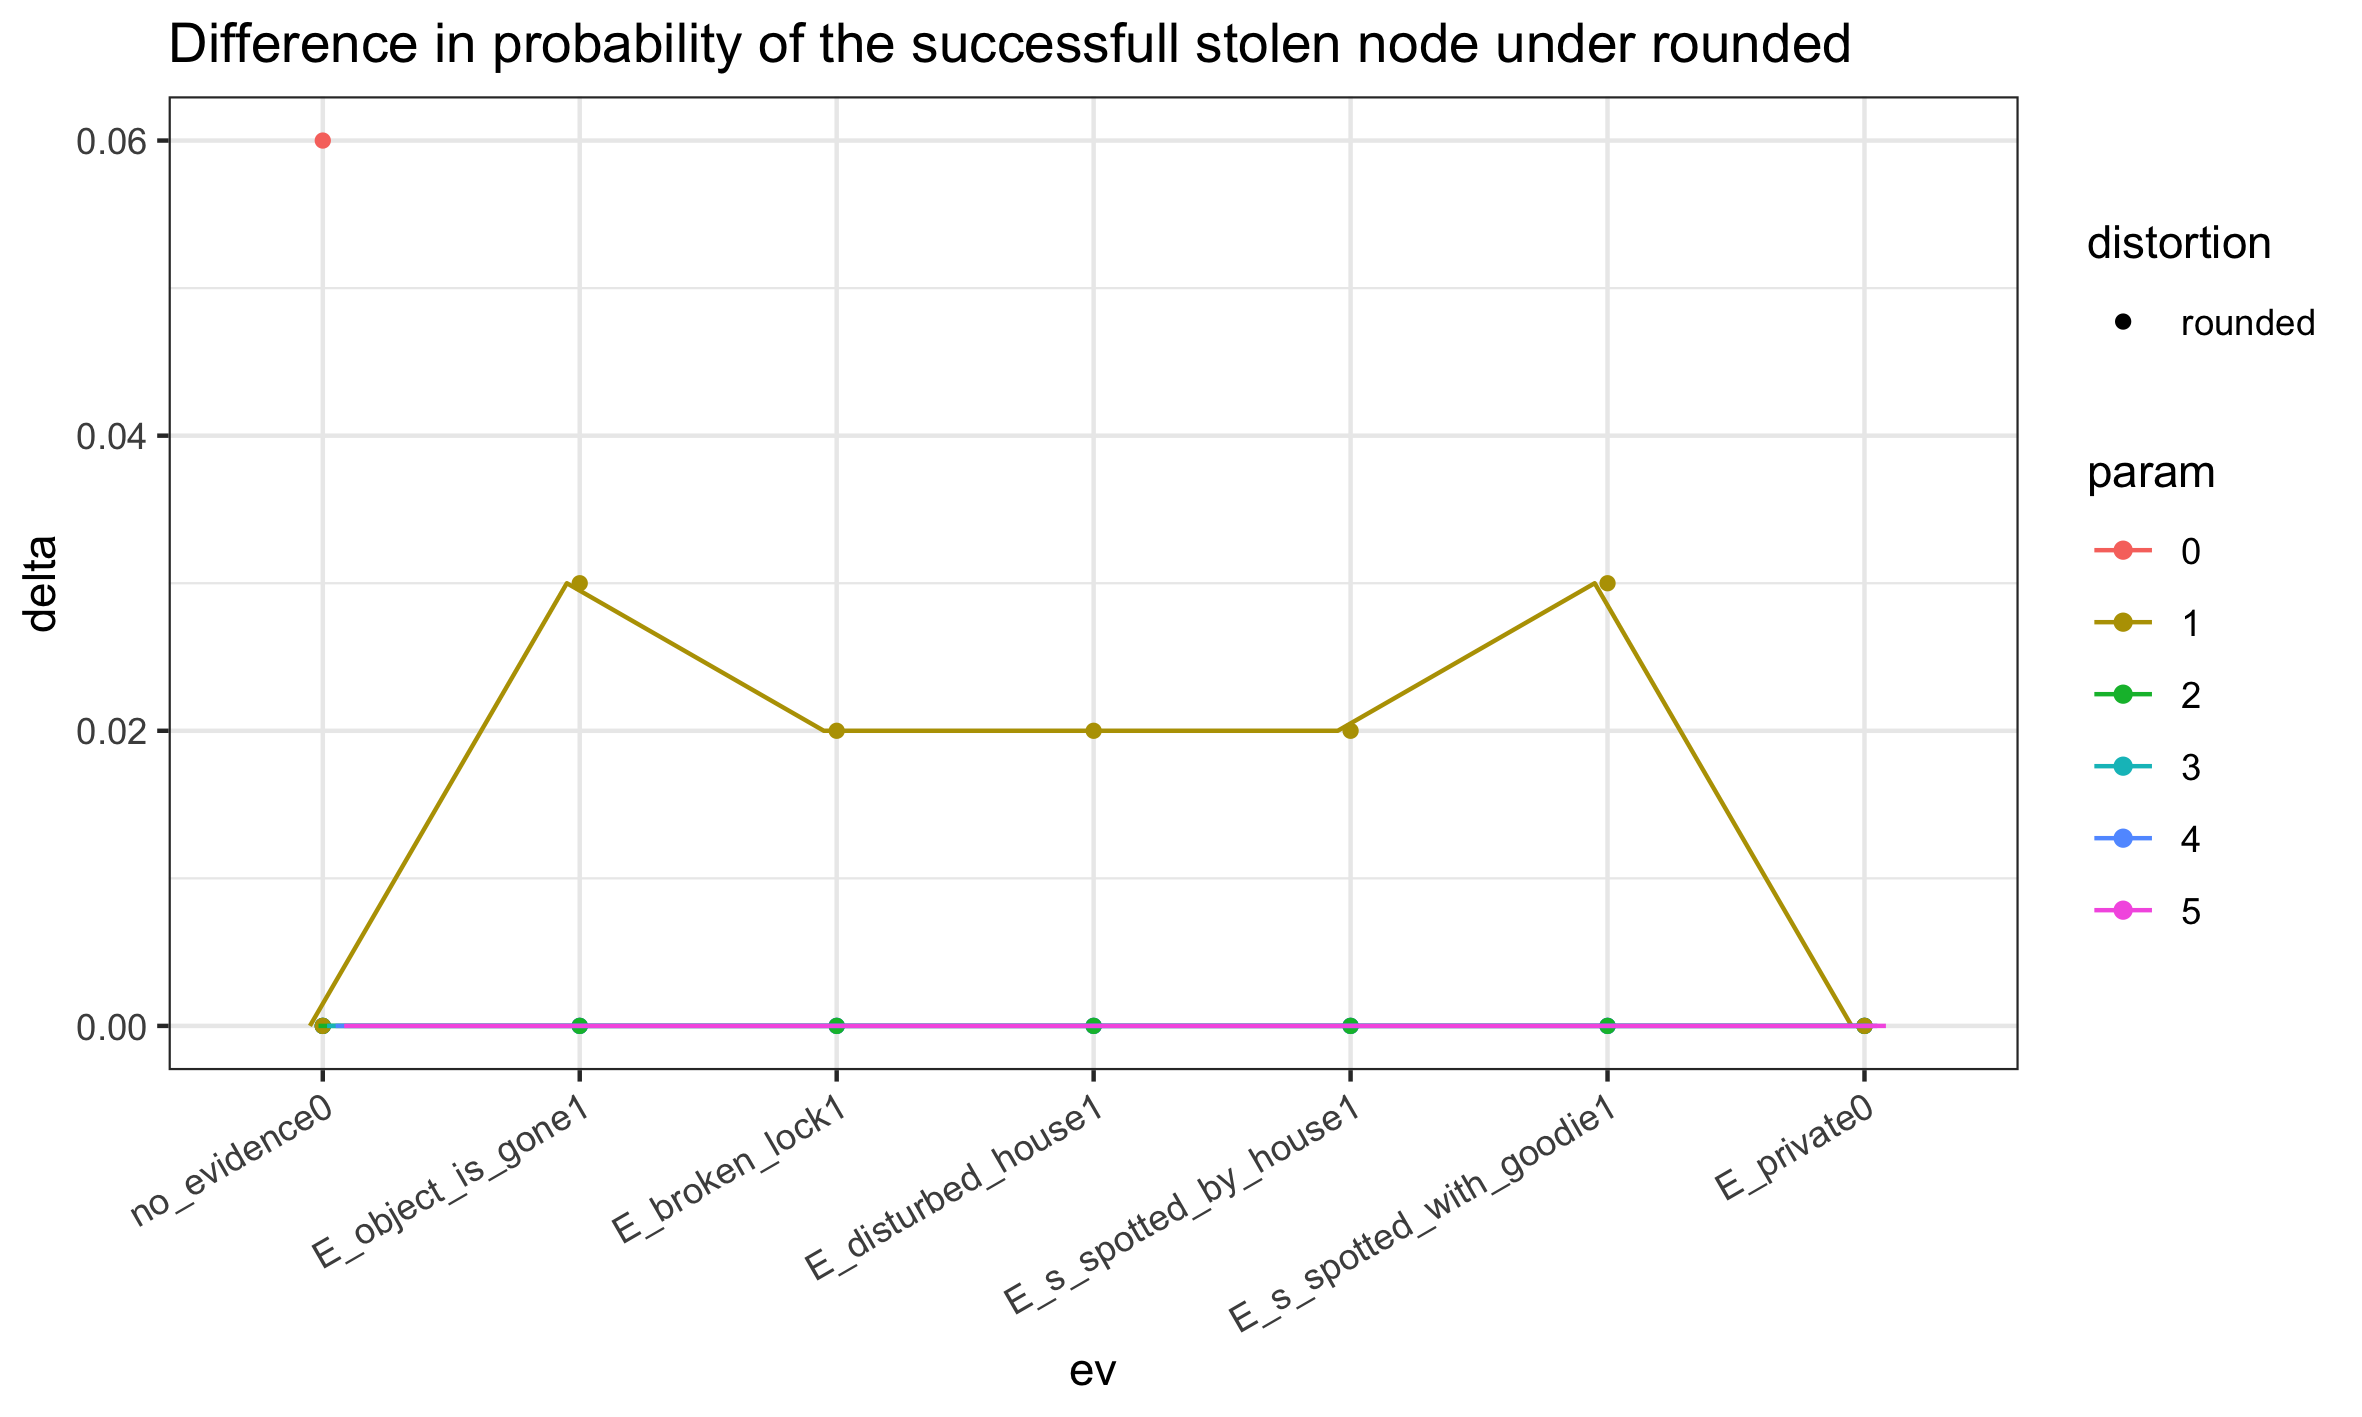
\includegraphics[scale=0.17]{images/roundeddelta.png}
\label{default}
\end{center}
\end{figure}

\begin{figure}[htbp]
\begin{center}
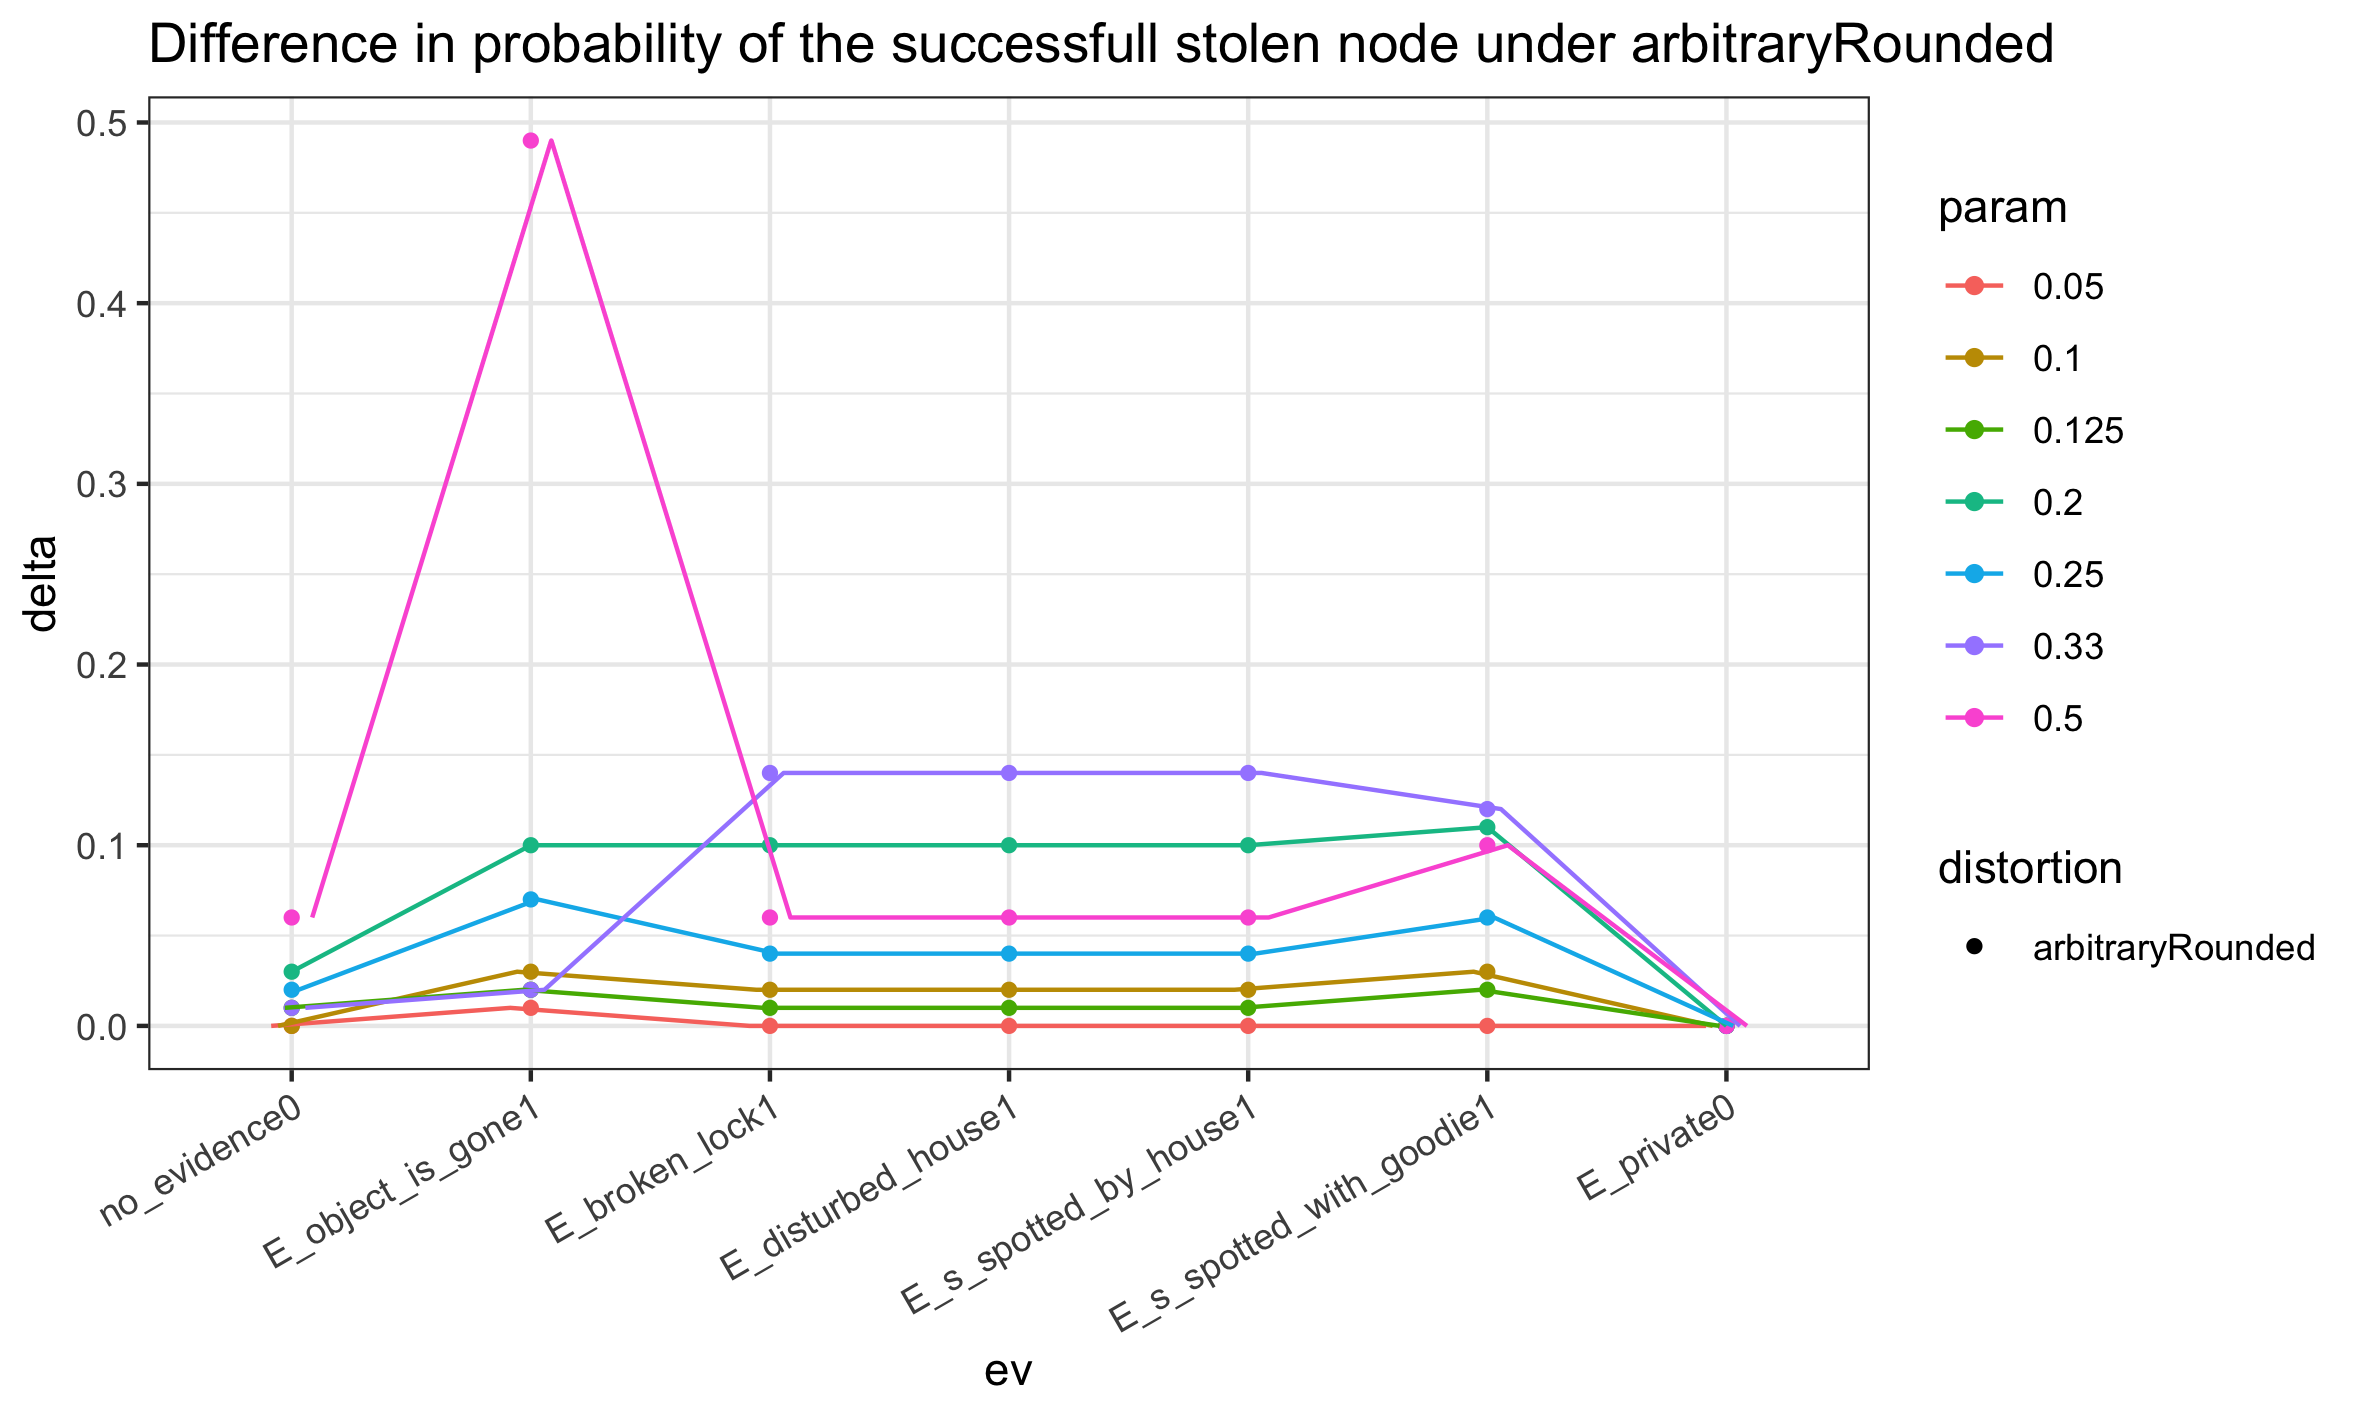
\includegraphics[scale=0.17]{images/arbitraryRoundeddelta.png}
\label{default}
\end{center}
\end{figure}

\begin{figure}[htbp]
\begin{center}
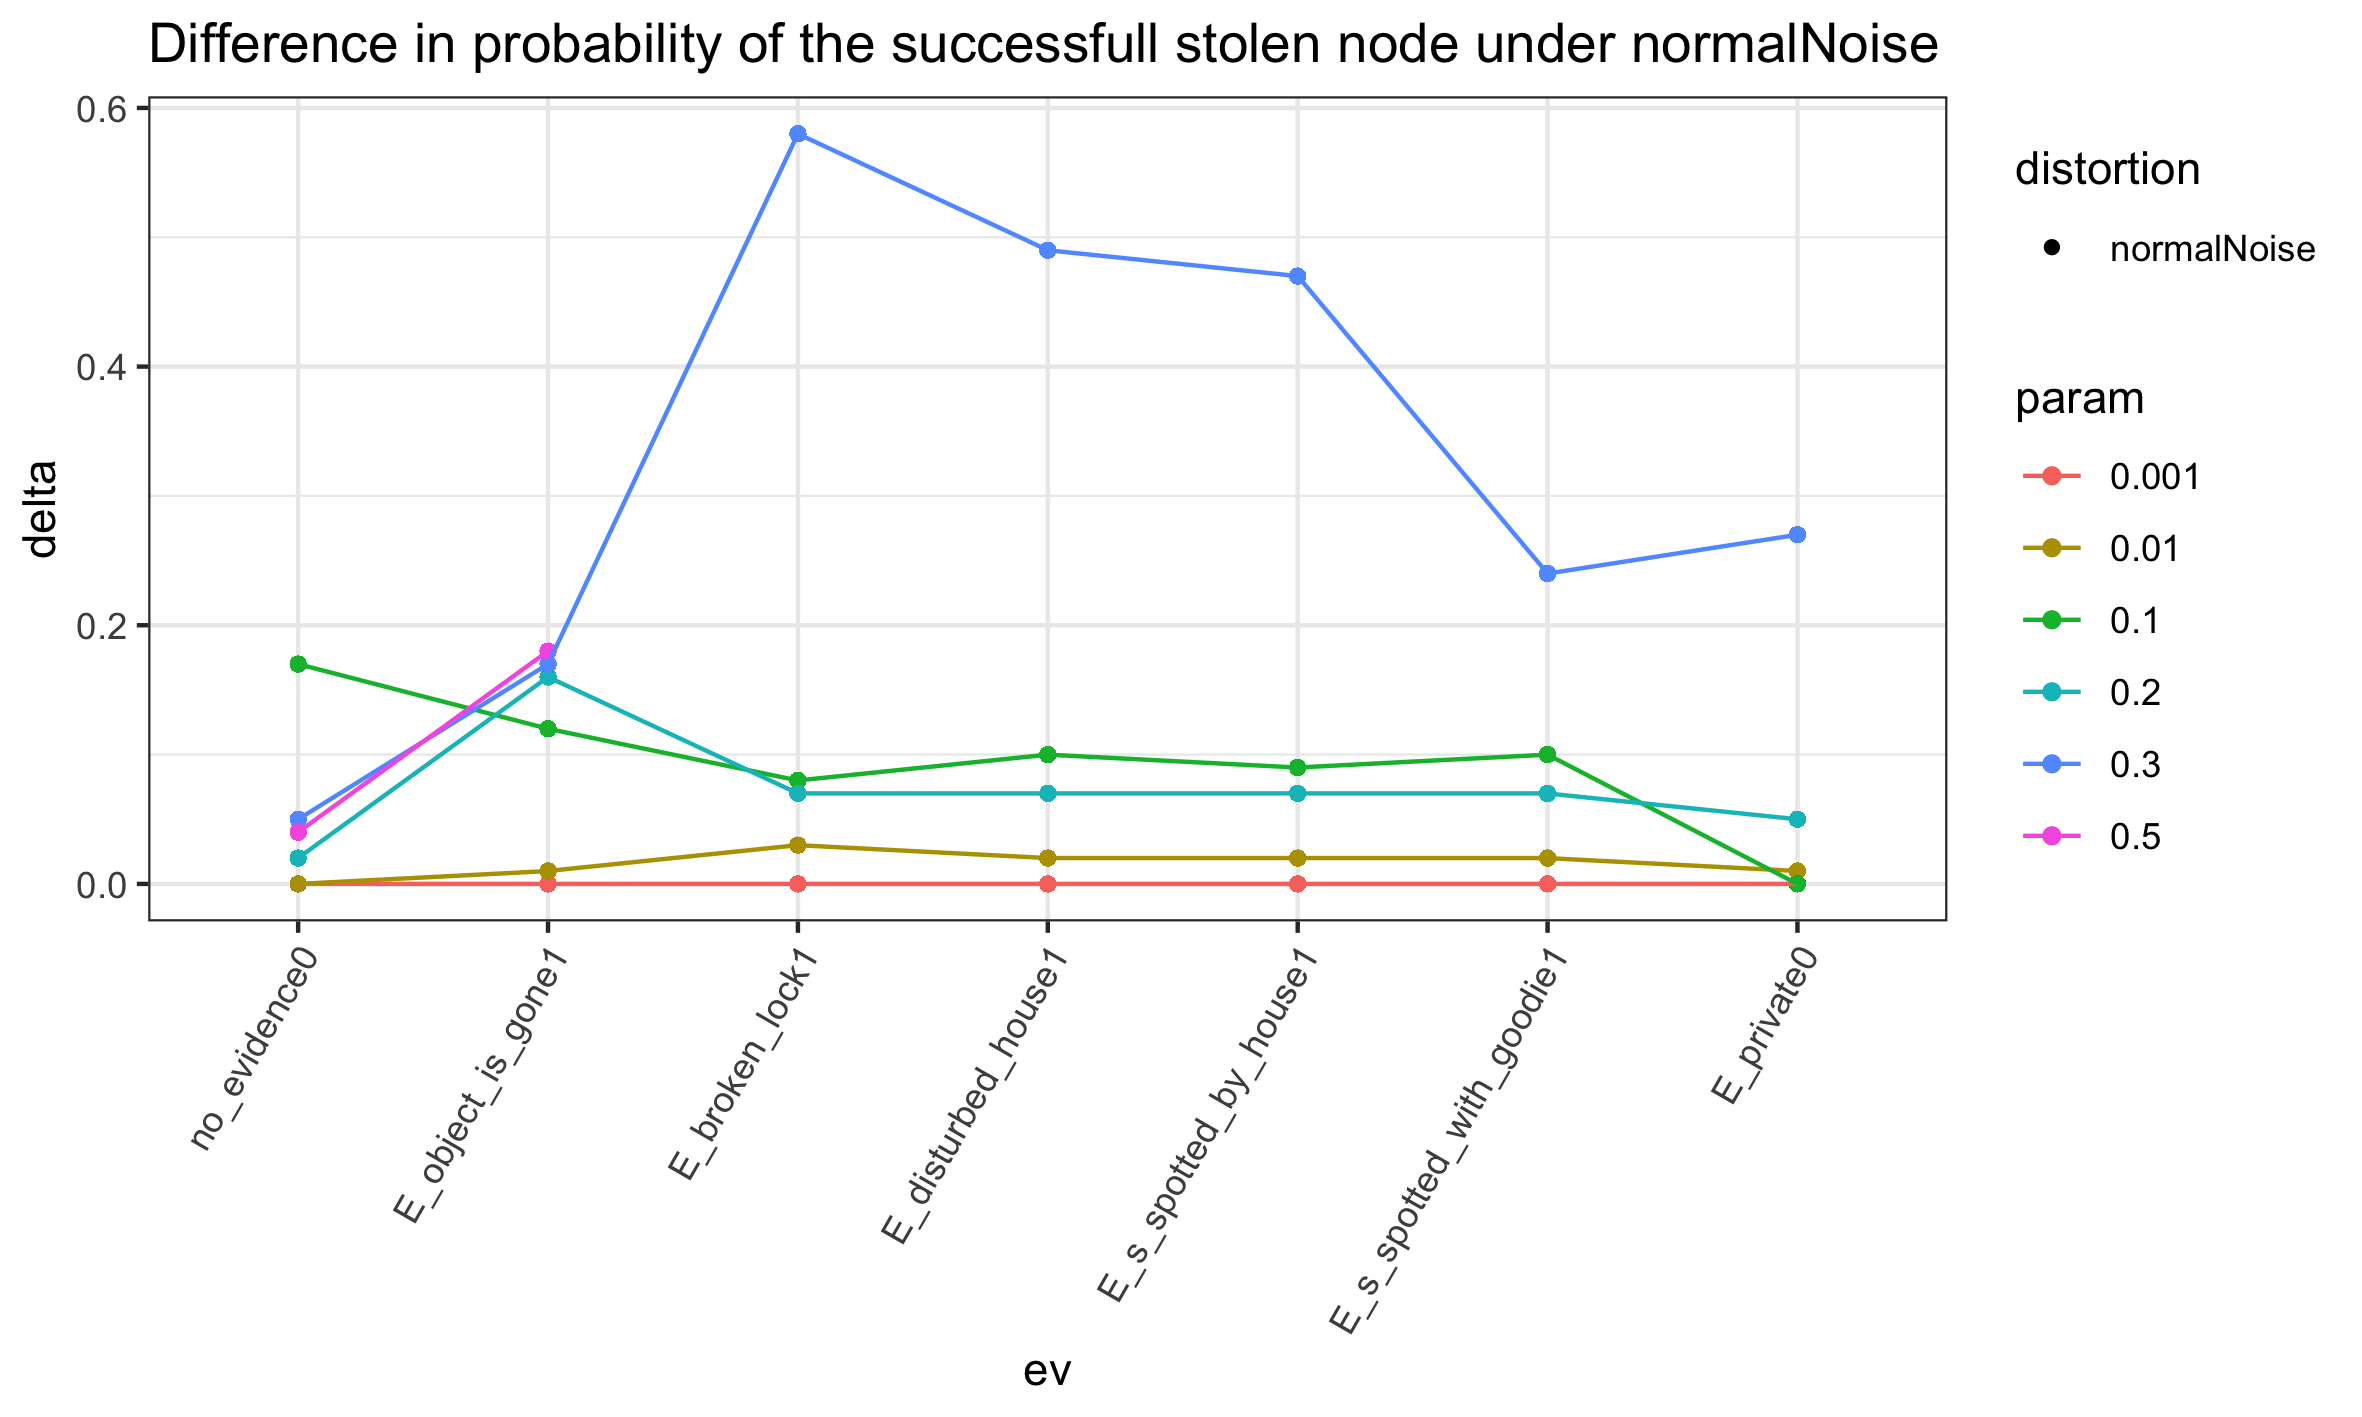
\includegraphics[scale=0.17]{images/normalNoisedelta.png}
\label{default}
\end{center}
\end{figure}


\clearpage

\section{Why we need hypothesis nodes!}
We need hypothesis nodes, since as you can see, when we round to an arbitrary level of precision (quarters, thirds), in a normal network, the differences between the disturbed and the original network, are relatively small (<0.2). 

However, if we leave out the hypothesis nodes, and only connect evidence directly to ``outcome'' nodes, you see that for larger intervals (so quarters, thirds and even seconds), the network gets into impossible states (NA). 

There's less tolerance here with rounding. If we have hypothesis nodes in between, we can still use quarters/thirds etc and get results that line up with the original network, instead of results that go to NA for degrees of precision that are lower than 0.2.

So with more hypothesis nodes you can be less precise in your exact probability assigning while still preserving the correct outcome. Which makes sense because you can condition on more stuff, you can probably make some calculation here but intuitively this makes sense, right - more hypothesis nodes allows for more nuance/larger truth table, and more conditional dependencies / more incoming arcs, so more complex calculation, hence more nuanced probability even if we constrain cpts to intervals.

\begin{figure}[htbp]
\begin{center}
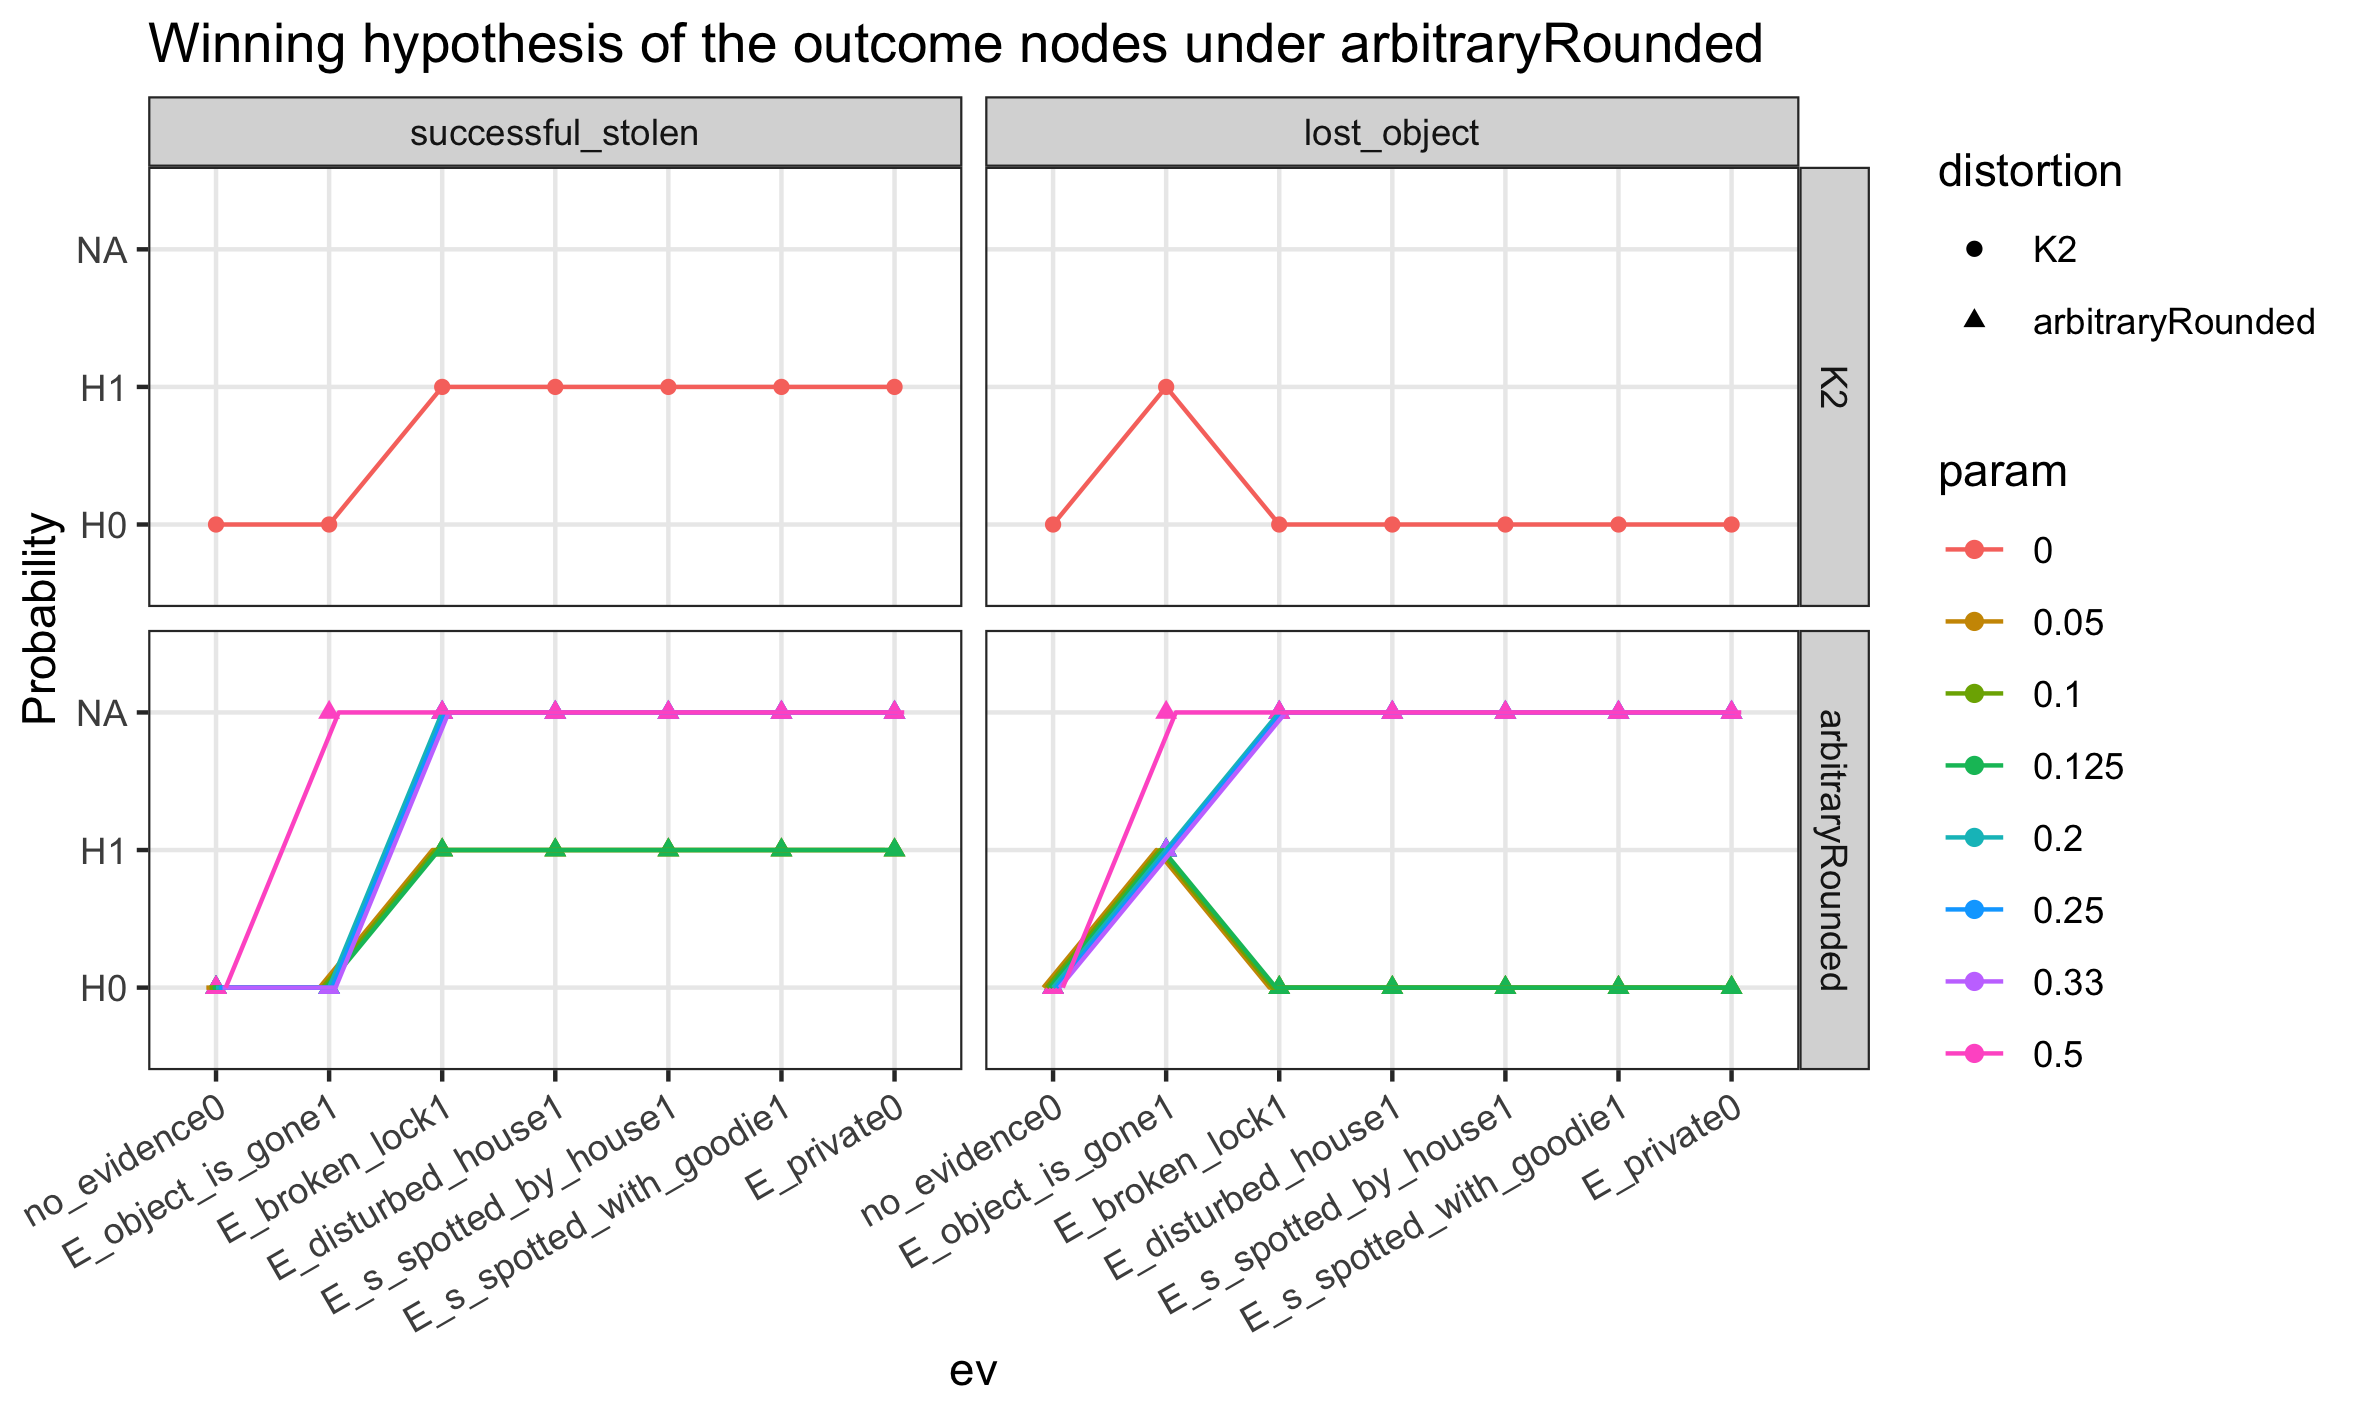
\includegraphics[scale=0.17]{images/arbitraryRoundedWeakSpider.png}
\label{default}
\end{center}
\end{figure}

\begin{figure}[htbp]
\begin{center}
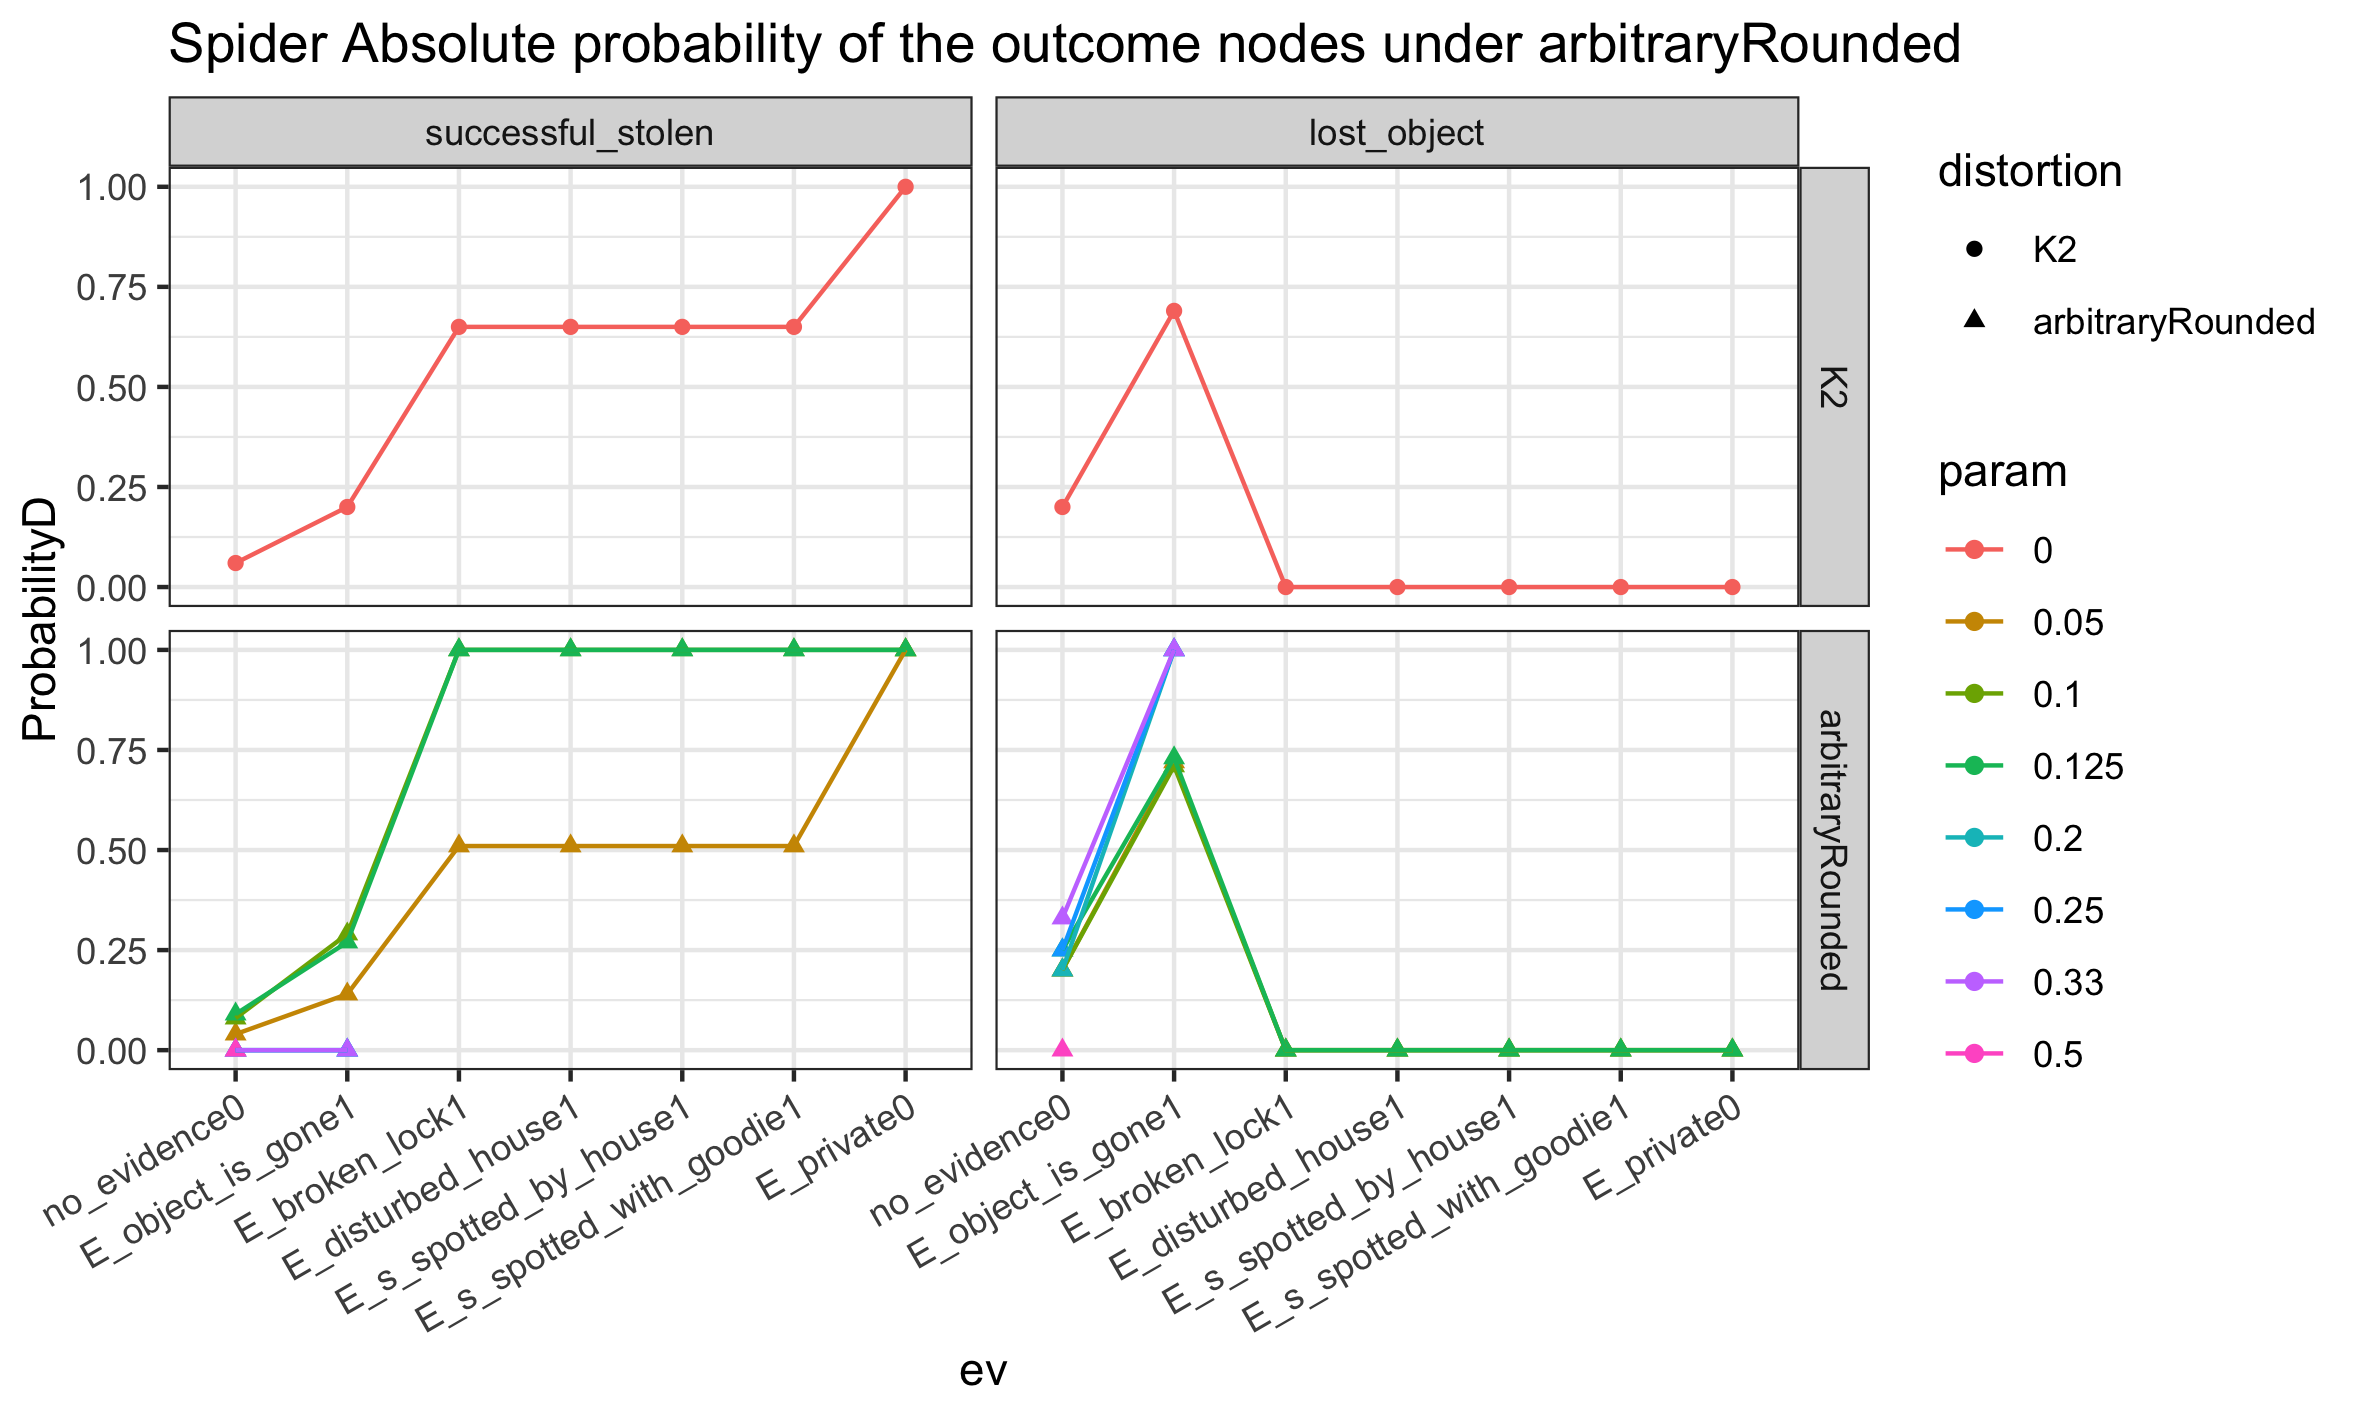
\includegraphics[scale=0.17]{images/strongarbitraryRoundedspider.png}
\label{default}
\end{center}
\end{figure}

\begin{figure}[htbp]
\begin{center}
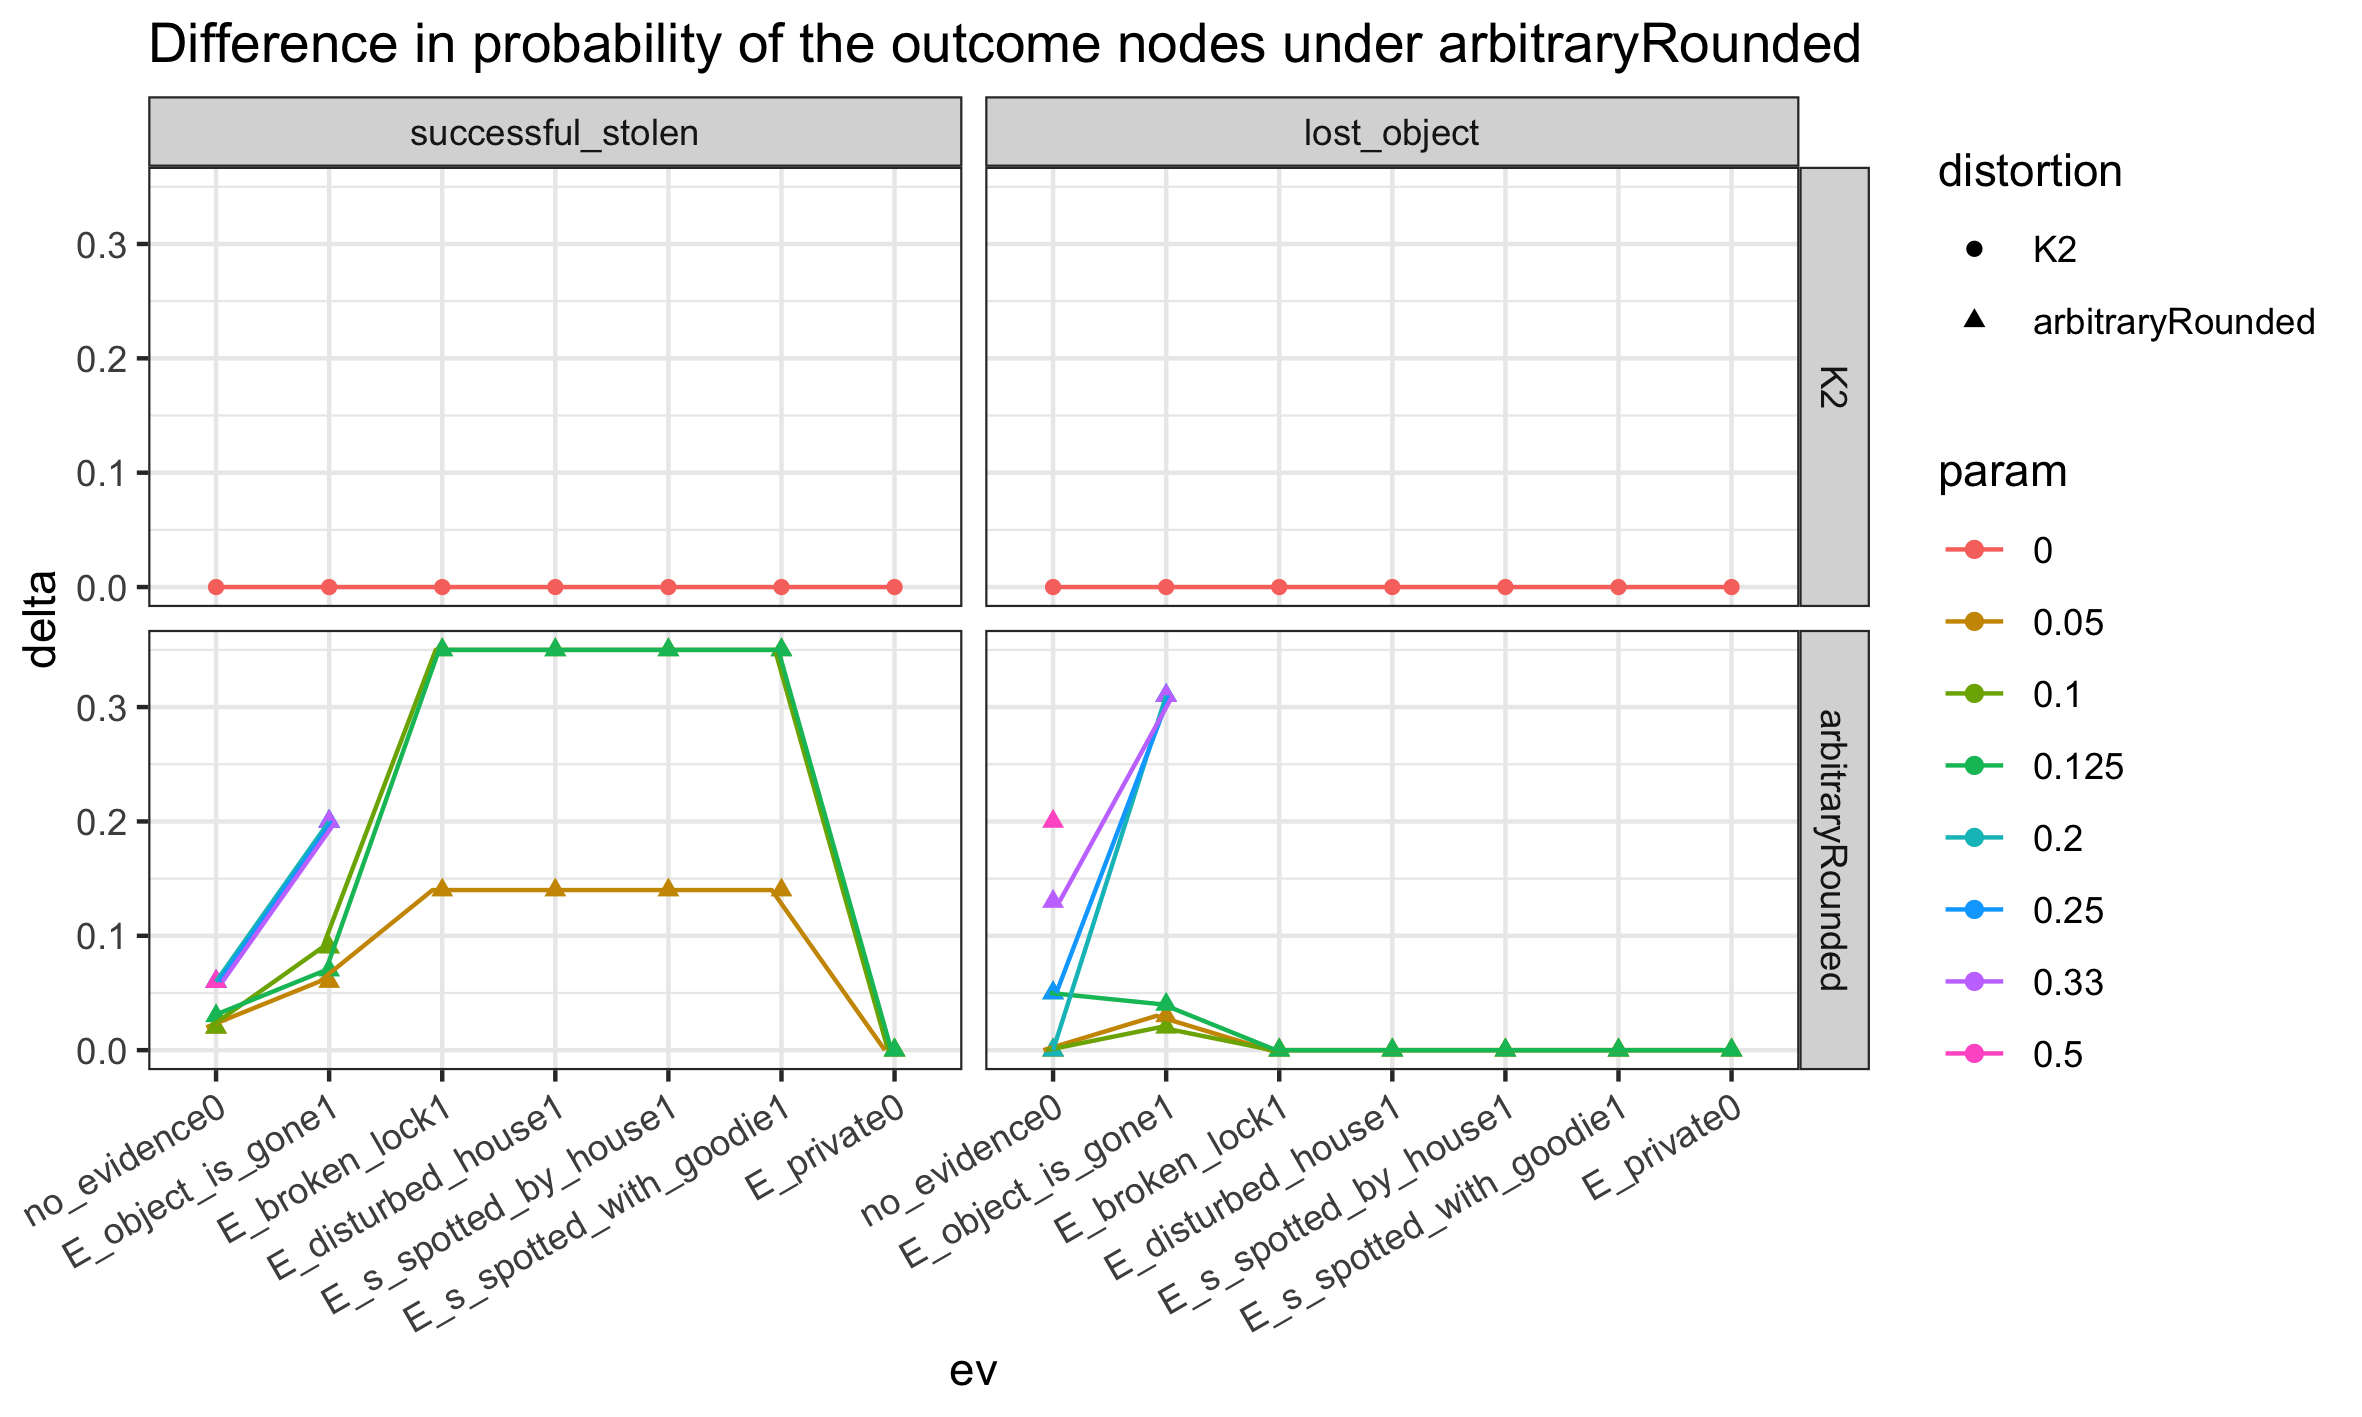
\includegraphics[scale=0.17]{images/arbitraryRoundeddeltaSpider.png}
\label{default}
\end{center}
\end{figure}

\section{TABLES: Effect of disturbing the cpts by removing precision with rounding}
\let\oldcentering\centering
\renewcommand\centering{\tiny\oldcentering}
\begin{table}\begin{tabular}{l|cc|cc}\toprule\multirow{2}{*}{Evidence} & \multicolumn{2}{c}{successful stolen}& \multicolumn{2}{c}{lost object}\\& {K2} & {Dev}& {K2} & {Dev}\\\midrule
no evidence, 0 & H0&H0&H0&H0\\E broken lock, 1 & H1&H1&H0&H0\\E object is gone, 1 & H1&H1&H0&H0\\E s spotted with goodie, 1 & H1&H1&H0&H0\\E disturbed house, 1 & H1&H1&H0&H0\\E s spotted by house, 1 & H1&H1&H0&H0\\E private, 0 & H1&H1&H0&H0\\\bottomrule\end{tabular}\caption{Effect of disturbance of [5, 'decimal places'] on weak view of hypotheses.}\end{table}
\begin{table}\begin{tabular}{l|cc|cc}\toprule\multirow{2}{*}{Evidence} & \multicolumn{2}{c}{successful stolen}& \multicolumn{2}{c}{lost object}\\& {K2} & {Dev}& {K2} & {Dev}\\\midrule
no evidence, 0 & H0&H0&H0&H0\\E broken lock, 1 & H1&H1&H0&H0\\E object is gone, 1 & H1&H1&H0&H0\\E s spotted with goodie, 1 & H1&H1&H0&H0\\E disturbed house, 1 & H1&H1&H0&H0\\E s spotted by house, 1 & H1&H1&H0&H0\\E private, 0 & H1&H1&H0&H0\\\bottomrule\end{tabular}\caption{Effect of disturbance of [5, 'decimal places'] on weak view of hypotheses.}\end{table}
\begin{table}\begin{tabular}{l|cc|cc}\toprule\multirow{2}{*}{Evidence} & \multicolumn{2}{c}{successful stolen}& \multicolumn{2}{c}{lost object}\\& {K2} & {Dev}& {K2} & {Dev}\\\midrule
no evidence, 0 & 0.06&0.06&0.19&0.19\\E object is gone, 1 & 0.2&0.2&0.68&0.68\\E broken lock, 1 & 0.62&0.62&0.0&0.0\\E disturbed house, 1 & 0.62&0.62&0.0&0.0\\E s spotted by house, 1 & 0.62&0.62&0.0&0.0\\E s spotted with goodie, 1 & 0.72&0.72&0.0&0.0\\E private, 0 & 1.0&1.0&0.0&0.0\\\bottomrule\end{tabular}\caption{Effect of disturbance of [5, 'decimal places'] on strong view of hypotheses.}\end{table}
\begin{table}\begin{tabular}{l|cc|cc}\toprule\multirow{2}{*}{Evidence} & \multicolumn{2}{c}{successful stolen}& \multicolumn{2}{c}{lost object}\\& {K2} & {Dev}& {K2} & {Dev}\\\midrule
no evidence, 0 & 0.06&0.06&0.19&0.19\\E object is gone, 1 & 0.2&0.2&0.68&0.68\\E broken lock, 1 & 0.62&0.62&0.0&0.0\\E disturbed house, 1 & 0.62&0.62&0.0&0.0\\E s spotted by house, 1 & 0.62&0.62&0.0&0.0\\E s spotted with goodie, 1 & 0.72&0.72&0.0&0.0\\E private, 0 & 1.0&1.0&0.0&0.0\\\bottomrule\end{tabular}\caption{Effect of disturbance of [5, 'decimal places'] on strong view of hypotheses.}\end{table}
\begin{table}\begin{tabular}{l|cc|cc}\toprule\multirow{2}{*}{Evidence} & \multicolumn{2}{c}{successful stolen}& \multicolumn{2}{c}{lost object}\\& {K2} & {Dev}& {K2} & {Dev}\\\midrule
no evidence, 0 & \cellcolor{Bittersweet}0.06&\cellcolor{Bittersweet}H0&\cellcolor{Bittersweet}0.19&\cellcolor{Bittersweet}H0\\E object is gone, 1 & \cellcolor{Bittersweet}0.2&\cellcolor{Bittersweet}H0&\cellcolor{Bittersweet}0.68&\cellcolor{Bittersweet}H1\\E broken lock, 1 & \cellcolor{Bittersweet}0.62&\cellcolor{Bittersweet}H1&\cellcolor{Bittersweet}0.0&\cellcolor{Bittersweet}H0\\E disturbed house, 1 & \cellcolor{Bittersweet}0.62&\cellcolor{Bittersweet}H1&\cellcolor{Bittersweet}0.0&\cellcolor{Bittersweet}H0\\E s spotted by house, 1 & \cellcolor{Bittersweet}0.62&\cellcolor{Bittersweet}H1&\cellcolor{Bittersweet}0.0&\cellcolor{Bittersweet}H0\\E s spotted with goodie, 1 & \cellcolor{Bittersweet}0.72&\cellcolor{Bittersweet}H1&\cellcolor{Bittersweet}0.0&\cellcolor{Bittersweet}H0\\E private, 0 & \cellcolor{Bittersweet}1.0&\cellcolor{Bittersweet}H1&\cellcolor{Bittersweet}0.0&\cellcolor{Bittersweet}H0\\\bottomrule\end{tabular}\caption{Effect of disturbance of [4, 'decimal places'] on weak view of hypotheses.}\end{table}
\begin{table}\begin{tabular}{l|cc|cc}\toprule\multirow{2}{*}{Evidence} & \multicolumn{2}{c}{successful stolen}& \multicolumn{2}{c}{lost object}\\& {K2} & {Dev}& {K2} & {Dev}\\\midrule
no evidence, 0 & \cellcolor{Bittersweet}0.06&\cellcolor{Bittersweet}H0&\cellcolor{Bittersweet}0.19&\cellcolor{Bittersweet}H0\\E object is gone, 1 & \cellcolor{Bittersweet}0.2&\cellcolor{Bittersweet}H0&\cellcolor{Bittersweet}0.68&\cellcolor{Bittersweet}H1\\E broken lock, 1 & \cellcolor{Bittersweet}0.62&\cellcolor{Bittersweet}H1&\cellcolor{Bittersweet}0.0&\cellcolor{Bittersweet}H0\\E disturbed house, 1 & \cellcolor{Bittersweet}0.62&\cellcolor{Bittersweet}H1&\cellcolor{Bittersweet}0.0&\cellcolor{Bittersweet}H0\\E s spotted by house, 1 & \cellcolor{Bittersweet}0.62&\cellcolor{Bittersweet}H1&\cellcolor{Bittersweet}0.0&\cellcolor{Bittersweet}H0\\E s spotted with goodie, 1 & \cellcolor{Bittersweet}0.72&\cellcolor{Bittersweet}H1&\cellcolor{Bittersweet}0.0&\cellcolor{Bittersweet}H0\\E private, 0 & \cellcolor{Bittersweet}1.0&\cellcolor{Bittersweet}H1&\cellcolor{Bittersweet}0.0&\cellcolor{Bittersweet}H0\\\bottomrule\end{tabular}\caption{Effect of disturbance of [4, 'decimal places'] on weak view of hypotheses.}\end{table}
\begin{table}\begin{tabular}{l|cc|cc}\toprule\multirow{2}{*}{Evidence} & \multicolumn{2}{c}{successful stolen}& \multicolumn{2}{c}{lost object}\\& {K2} & {Dev}& {K2} & {Dev}\\\midrule
no evidence, 0 & 0.06&0.06&0.24&0.24\\E broken lock, 1 & 0.57&0.57&0.03&0.03\\E object is gone, 1 & 0.58&0.58&0.01&0.01\\E s spotted with goodie, 1 & 1.0&1.0&0.0&0.0\\E disturbed house, 1 & 1.0&1.0&0.0&0.0\\E s spotted by house, 1 & 1.0&1.0&0.0&0.0\\E private, 0 & 1.0&1.0&0.0&0.0\\\bottomrule\end{tabular}\caption{Effect of disturbance of [4, 'decimal places'] on strong view of hypotheses.}\end{table}
\begin{table}\begin{tabular}{l|cc|cc}\toprule\multirow{2}{*}{Evidence} & \multicolumn{2}{c}{successful stolen}& \multicolumn{2}{c}{lost object}\\& {K2} & {Dev}& {K2} & {Dev}\\\midrule
no evidence, 0 & 0.06&0.06&0.24&0.24\\E broken lock, 1 & 0.57&0.57&0.03&0.03\\E object is gone, 1 & 0.58&0.58&0.01&0.01\\E s spotted with goodie, 1 & 1.0&1.0&0.0&0.0\\E disturbed house, 1 & 1.0&1.0&0.0&0.0\\E s spotted by house, 1 & 1.0&1.0&0.0&0.0\\E private, 0 & 1.0&1.0&0.0&0.0\\\bottomrule\end{tabular}\caption{Effect of disturbance of [4, 'decimal places'] on strong view of hypotheses.}\end{table}
\begin{table}\begin{tabular}{l|cc|cc|cc|cc|cc|cc|cc}\toprule\multirow{2}{*}{Evidence} & \multicolumn{2}{c}{flees startled}& \multicolumn{2}{c}{raining}& \multicolumn{2}{c}{curtains}& \multicolumn{2}{c}{motive}& \multicolumn{2}{c}{compromise house}& \multicolumn{2}{c}{target object}& \multicolumn{2}{c}{know object}\\& {K2} & {Dev}& {K2} & {Dev}& {K2} & {Dev}& {K2} & {Dev}& {K2} & {Dev}& {K2} & {Dev}& {K2} & {Dev}\\\midrule
no evidence, 0 & \cellcolor{Bittersweet}0.16&\cellcolor{Bittersweet}H0&\cellcolor{Bittersweet}0.51&\cellcolor{Bittersweet}H1&\cellcolor{Bittersweet}0.18&\cellcolor{Bittersweet}H0&\cellcolor{Bittersweet}0.32&\cellcolor{Bittersweet}H0&\cellcolor{Bittersweet}0.11&\cellcolor{Bittersweet}H0&\cellcolor{Bittersweet}0.32&\cellcolor{Bittersweet}H0&\cellcolor{Bittersweet}0.64&\cellcolor{Bittersweet}H1\\E object is gone, 1 & \cellcolor{Bittersweet}0.12&\cellcolor{Bittersweet}H0&\cellcolor{Bittersweet}0.52&\cellcolor{Bittersweet}H1&\cellcolor{Bittersweet}0.12&\cellcolor{Bittersweet}H0&\cellcolor{Bittersweet}0.32&\cellcolor{Bittersweet}H0&\cellcolor{Bittersweet}0.32&\cellcolor{Bittersweet}H0&\cellcolor{Bittersweet}0.32&\cellcolor{Bittersweet}H0&\cellcolor{Bittersweet}0.32&\cellcolor{Bittersweet}H0\\E broken lock, 1 & \cellcolor{Bittersweet}0.38&\cellcolor{Bittersweet}H0&\cellcolor{Bittersweet}0.55&\cellcolor{Bittersweet}H1&\cellcolor{Bittersweet}0.0&\cellcolor{Bittersweet}H0&\cellcolor{Bittersweet}1.0&\cellcolor{Bittersweet}H1&\cellcolor{Bittersweet}1.0&\cellcolor{Bittersweet}H1&\cellcolor{Bittersweet}1.0&\cellcolor{Bittersweet}H1&\cellcolor{Bittersweet}1.0&\cellcolor{Bittersweet}H1\\E disturbed house, 1 & \cellcolor{Bittersweet}0.38&\cellcolor{Bittersweet}H0&\cellcolor{Bittersweet}0.55&\cellcolor{Bittersweet}H1&\cellcolor{Bittersweet}0.0&\cellcolor{Bittersweet}H0&\cellcolor{Bittersweet}1.0&\cellcolor{Bittersweet}H1&\cellcolor{Bittersweet}1.0&\cellcolor{Bittersweet}H1&\cellcolor{Bittersweet}1.0&\cellcolor{Bittersweet}H1&\cellcolor{Bittersweet}1.0&\cellcolor{Bittersweet}H1\\E s spotted by house, 1 & \cellcolor{Bittersweet}0.38&\cellcolor{Bittersweet}H0&\cellcolor{Bittersweet}0.55&\cellcolor{Bittersweet}H1&\cellcolor{Bittersweet}0.0&\cellcolor{Bittersweet}H0&\cellcolor{Bittersweet}1.0&\cellcolor{Bittersweet}H1&\cellcolor{Bittersweet}1.0&\cellcolor{Bittersweet}H1&\cellcolor{Bittersweet}1.0&\cellcolor{Bittersweet}H1&\cellcolor{Bittersweet}1.0&\cellcolor{Bittersweet}H1\\E s spotted with goodie, 1 & \cellcolor{Bittersweet}0.29&\cellcolor{Bittersweet}H0&\cellcolor{Bittersweet}0.55&\cellcolor{Bittersweet}H1&\cellcolor{Bittersweet}0.0&\cellcolor{Bittersweet}H0&\cellcolor{Bittersweet}1.0&\cellcolor{Bittersweet}H1&\cellcolor{Bittersweet}1.0&\cellcolor{Bittersweet}H1&\cellcolor{Bittersweet}1.0&\cellcolor{Bittersweet}H1&\cellcolor{Bittersweet}1.0&\cellcolor{Bittersweet}H1\\E private, 0 & \cellcolor{Bittersweet}0.0&\cellcolor{Bittersweet}H0&\cellcolor{Bittersweet}0.55&\cellcolor{Bittersweet}H1&\cellcolor{Bittersweet}0.0&\cellcolor{Bittersweet}H0&\cellcolor{Bittersweet}1.0&\cellcolor{Bittersweet}H1&\cellcolor{Bittersweet}1.0&\cellcolor{Bittersweet}H1&\cellcolor{Bittersweet}1.0&\cellcolor{Bittersweet}H1&\cellcolor{Bittersweet}1.0&\cellcolor{Bittersweet}H1\\\bottomrule\end{tabular}\caption{Effect of disturbance of [3, 'decimal places'] on weak view of outcomes.}\end{table}
\begin{table}\begin{tabular}{l|cc|cc|cc|cc|cc|cc|cc}\toprule\multirow{2}{*}{Evidence} & \multicolumn{2}{c}{flees startled}& \multicolumn{2}{c}{raining}& \multicolumn{2}{c}{curtains}& \multicolumn{2}{c}{motive}& \multicolumn{2}{c}{compromise house}& \multicolumn{2}{c}{target object}& \multicolumn{2}{c}{know object}\\& {K2} & {Dev}& {K2} & {Dev}& {K2} & {Dev}& {K2} & {Dev}& {K2} & {Dev}& {K2} & {Dev}& {K2} & {Dev}\\\midrule
no evidence, 0 & \cellcolor{Bittersweet}0.16&\cellcolor{Bittersweet}H0&\cellcolor{Bittersweet}0.51&\cellcolor{Bittersweet}H1&\cellcolor{Bittersweet}0.18&\cellcolor{Bittersweet}H0&\cellcolor{Bittersweet}0.32&\cellcolor{Bittersweet}H0&\cellcolor{Bittersweet}0.11&\cellcolor{Bittersweet}H0&\cellcolor{Bittersweet}0.32&\cellcolor{Bittersweet}H0&\cellcolor{Bittersweet}0.64&\cellcolor{Bittersweet}H1\\E object is gone, 1 & \cellcolor{Bittersweet}0.12&\cellcolor{Bittersweet}H0&\cellcolor{Bittersweet}0.52&\cellcolor{Bittersweet}H1&\cellcolor{Bittersweet}0.12&\cellcolor{Bittersweet}H0&\cellcolor{Bittersweet}0.32&\cellcolor{Bittersweet}H0&\cellcolor{Bittersweet}0.32&\cellcolor{Bittersweet}H0&\cellcolor{Bittersweet}0.32&\cellcolor{Bittersweet}H0&\cellcolor{Bittersweet}0.32&\cellcolor{Bittersweet}H0\\E broken lock, 1 & \cellcolor{Bittersweet}0.38&\cellcolor{Bittersweet}H0&\cellcolor{Bittersweet}0.55&\cellcolor{Bittersweet}H1&\cellcolor{Bittersweet}0.0&\cellcolor{Bittersweet}H0&\cellcolor{Bittersweet}1.0&\cellcolor{Bittersweet}H1&\cellcolor{Bittersweet}1.0&\cellcolor{Bittersweet}H1&\cellcolor{Bittersweet}1.0&\cellcolor{Bittersweet}H1&\cellcolor{Bittersweet}1.0&\cellcolor{Bittersweet}H1\\E disturbed house, 1 & \cellcolor{Bittersweet}0.38&\cellcolor{Bittersweet}H0&\cellcolor{Bittersweet}0.55&\cellcolor{Bittersweet}H1&\cellcolor{Bittersweet}0.0&\cellcolor{Bittersweet}H0&\cellcolor{Bittersweet}1.0&\cellcolor{Bittersweet}H1&\cellcolor{Bittersweet}1.0&\cellcolor{Bittersweet}H1&\cellcolor{Bittersweet}1.0&\cellcolor{Bittersweet}H1&\cellcolor{Bittersweet}1.0&\cellcolor{Bittersweet}H1\\E s spotted by house, 1 & \cellcolor{Bittersweet}0.38&\cellcolor{Bittersweet}H0&\cellcolor{Bittersweet}0.55&\cellcolor{Bittersweet}H1&\cellcolor{Bittersweet}0.0&\cellcolor{Bittersweet}H0&\cellcolor{Bittersweet}1.0&\cellcolor{Bittersweet}H1&\cellcolor{Bittersweet}1.0&\cellcolor{Bittersweet}H1&\cellcolor{Bittersweet}1.0&\cellcolor{Bittersweet}H1&\cellcolor{Bittersweet}1.0&\cellcolor{Bittersweet}H1\\E s spotted with goodie, 1 & \cellcolor{Bittersweet}0.29&\cellcolor{Bittersweet}H0&\cellcolor{Bittersweet}0.55&\cellcolor{Bittersweet}H1&\cellcolor{Bittersweet}0.0&\cellcolor{Bittersweet}H0&\cellcolor{Bittersweet}1.0&\cellcolor{Bittersweet}H1&\cellcolor{Bittersweet}1.0&\cellcolor{Bittersweet}H1&\cellcolor{Bittersweet}1.0&\cellcolor{Bittersweet}H1&\cellcolor{Bittersweet}1.0&\cellcolor{Bittersweet}H1\\E private, 0 & \cellcolor{Bittersweet}0.0&\cellcolor{Bittersweet}H0&\cellcolor{Bittersweet}0.55&\cellcolor{Bittersweet}H1&\cellcolor{Bittersweet}0.0&\cellcolor{Bittersweet}H0&\cellcolor{Bittersweet}1.0&\cellcolor{Bittersweet}H1&\cellcolor{Bittersweet}1.0&\cellcolor{Bittersweet}H1&\cellcolor{Bittersweet}1.0&\cellcolor{Bittersweet}H1&\cellcolor{Bittersweet}1.0&\cellcolor{Bittersweet}H1\\\bottomrule\end{tabular}\caption{Effect of disturbance of [3, 'decimal places'] on weak view of outcomes.}\end{table}
\begin{table}\begin{tabular}{l|cc|cc}\toprule\multirow{2}{*}{Evidence} & \multicolumn{2}{c}{successful stolen}& \multicolumn{2}{c}{lost object}\\& {K2} & {Dev}& {K2} & {Dev}\\\midrule
no evidence, 0 & 0.06&0.06&0.19&0.19\\E object is gone, 1 & 0.2&0.2&0.68&0.68\\E broken lock, 1 & 0.62&0.62&0.0&0.0\\E disturbed house, 1 & 0.62&0.62&0.0&0.0\\E s spotted by house, 1 & 0.62&0.62&0.0&0.0\\E s spotted with goodie, 1 & 0.72&0.72&0.0&0.0\\E private, 0 & 1.0&1.0&0.0&0.0\\\bottomrule\end{tabular}\caption{Effect of disturbance of [3, 'decimal places'] on strong view of hypotheses.}\end{table}
\begin{table}\begin{tabular}{l|cc|cc}\toprule\multirow{2}{*}{Evidence} & \multicolumn{2}{c}{successful stolen}& \multicolumn{2}{c}{lost object}\\& {K2} & {Dev}& {K2} & {Dev}\\\midrule
no evidence, 0 & 0.06&0.06&0.19&0.19\\E object is gone, 1 & 0.2&0.2&0.68&0.68\\E broken lock, 1 & 0.62&0.62&0.0&0.0\\E disturbed house, 1 & 0.62&0.62&0.0&0.0\\E s spotted by house, 1 & 0.62&0.62&0.0&0.0\\E s spotted with goodie, 1 & 0.72&0.72&0.0&0.0\\E private, 0 & 1.0&1.0&0.0&0.0\\\bottomrule\end{tabular}\caption{Effect of disturbance of [3, 'decimal places'] on strong view of hypotheses.}\end{table}
\begin{table}\begin{tabular}{l|cc|cc}\toprule\multirow{2}{*}{Evidence} & \multicolumn{2}{c}{successful stolen}& \multicolumn{2}{c}{lost object}\\& {K2} & {Dev}& {K2} & {Dev}\\\midrule
no evidence, 0 & H0&H0&H0&H0\\E broken lock, 1 & H1&H1&H0&H0\\E object is gone, 1 & H1&H1&H0&H0\\E s spotted with goodie, 1 & H1&H1&H0&H0\\E disturbed house, 1 & H1&H1&H0&H0\\E s spotted by house, 1 & H1&H1&H0&H0\\E private, 0 & H1&H1&H0&H0\\\bottomrule\end{tabular}\caption{Effect of disturbance of [2, 'decimal places'] on weak view of hypotheses.}\end{table}
\begin{table}\begin{tabular}{l|cc|cc}\toprule\multirow{2}{*}{Evidence} & \multicolumn{2}{c}{successful stolen}& \multicolumn{2}{c}{lost object}\\& {K2} & {Dev}& {K2} & {Dev}\\\midrule
no evidence, 0 & H0&H0&H0&H0\\E broken lock, 1 & H1&H1&H0&H0\\E object is gone, 1 & H1&H1&H0&H0\\E s spotted with goodie, 1 & H1&H1&H0&H0\\E disturbed house, 1 & H1&H1&H0&H0\\E s spotted by house, 1 & H1&H1&H0&H0\\E private, 0 & H1&H1&H0&H0\\\bottomrule\end{tabular}\caption{Effect of disturbance of [2, 'decimal places'] on weak view of hypotheses.}\end{table}
\begin{table}\begin{tabular}{l|cc|cc}\toprule\multirow{2}{*}{Evidence} & \multicolumn{2}{c}{successful stolen}& \multicolumn{2}{c}{lost object}\\& {K2} & {Dev}& {K2} & {Dev}\\\midrule
no evidence, 0 & 0.06&0.06&0.19&0.19\\E object is gone, 1 & 0.2&0.2&0.68&0.68\\E broken lock, 1 & 0.62&0.62&0.0&0.0\\E disturbed house, 1 & 0.62&0.62&0.0&0.0\\E s spotted by house, 1 & 0.62&0.62&0.0&0.0\\E s spotted with goodie, 1 & 0.72&0.71&0.0&0.0\\E private, 0 & 1.0&1.0&0.0&0.0\\\bottomrule\end{tabular}\caption{Effect of disturbance of [2, 'decimal places'] on strong view of hypotheses.}\end{table}
\begin{table}\begin{tabular}{l|cc|cc}\toprule\multirow{2}{*}{Evidence} & \multicolumn{2}{c}{successful stolen}& \multicolumn{2}{c}{lost object}\\& {K2} & {Dev}& {K2} & {Dev}\\\midrule
no evidence, 0 & 0.06&0.06&0.19&0.19\\E object is gone, 1 & 0.2&0.2&0.68&0.68\\E broken lock, 1 & 0.62&0.62&0.0&0.0\\E disturbed house, 1 & 0.62&0.62&0.0&0.0\\E s spotted by house, 1 & 0.62&0.62&0.0&0.0\\E s spotted with goodie, 1 & 0.72&0.71&0.0&0.0\\E private, 0 & 1.0&1.0&0.0&0.0\\\bottomrule\end{tabular}\caption{Effect of disturbance of [2, 'decimal places'] on strong view of hypotheses.}\end{table}
\begin{table}\begin{tabular}{l|cc|cc|cc|cc|cc|cc|cc}\toprule\multirow{2}{*}{Evidence} & \multicolumn{2}{c}{know object}& \multicolumn{2}{c}{curtains}& \multicolumn{2}{c}{raining}& \multicolumn{2}{c}{target object}& \multicolumn{2}{c}{compromise house}& \multicolumn{2}{c}{flees startled}& \multicolumn{2}{c}{motive}\\& {K2} & {Dev}& {K2} & {Dev}& {K2} & {Dev}& {K2} & {Dev}& {K2} & {Dev}& {K2} & {Dev}& {K2} & {Dev}\\\midrule
no evidence, 0 & H1&H1&H0&H0&H1&H1&H0&H0&H0&H0&H0&H0&H0&H0\\E broken lock, 1 & H1&H1&H0&H0&H1&H1&H1&H1&H1&H1&H0&H0&H1&H1\\E object is gone, 1 & H1&H1&H0&H0&H1&H1&H1&H1&H1&H1&H0&H0&H1&H1\\E s spotted with goodie, 1 & H1&H1&H0&H0&H1&H1&H1&H1&H1&H1&H0&H0&H1&H1\\E disturbed house, 1 & H1&H1&H0&H0&H1&H1&H1&H1&H1&H1&H0&H0&H1&H1\\E s spotted by house, 1 & H1&H1&H0&H0&H1&H1&H1&H1&H1&H1&H0&H0&H1&H1\\E private, 0 & H1&H1&H0&H0&H1&H1&H1&H1&H1&H1&H0&H0&H1&H1\\\bottomrule\end{tabular}\caption{Effect of disturbance of [1, 'decimal places'] on weak view of outcomes.}\end{table}
\begin{table}\begin{tabular}{l|cc|cc|cc|cc|cc|cc|cc}\toprule\multirow{2}{*}{Evidence} & \multicolumn{2}{c}{know object}& \multicolumn{2}{c}{curtains}& \multicolumn{2}{c}{raining}& \multicolumn{2}{c}{target object}& \multicolumn{2}{c}{compromise house}& \multicolumn{2}{c}{flees startled}& \multicolumn{2}{c}{motive}\\& {K2} & {Dev}& {K2} & {Dev}& {K2} & {Dev}& {K2} & {Dev}& {K2} & {Dev}& {K2} & {Dev}& {K2} & {Dev}\\\midrule
no evidence, 0 & H1&H1&H0&H0&H1&H1&H0&H0&H0&H0&H0&H0&H0&H0\\E broken lock, 1 & H1&H1&H0&H0&H1&H1&H1&H1&H1&H1&H0&H0&H1&H1\\E object is gone, 1 & H1&H1&H0&H0&H1&H1&H1&H1&H1&H1&H0&H0&H1&H1\\E s spotted with goodie, 1 & H1&H1&H0&H0&H1&H1&H1&H1&H1&H1&H0&H0&H1&H1\\E disturbed house, 1 & H1&H1&H0&H0&H1&H1&H1&H1&H1&H1&H0&H0&H1&H1\\E s spotted by house, 1 & H1&H1&H0&H0&H1&H1&H1&H1&H1&H1&H0&H0&H1&H1\\E private, 0 & H1&H1&H0&H0&H1&H1&H1&H1&H1&H1&H0&H0&H1&H1\\\bottomrule\end{tabular}\caption{Effect of disturbance of [1, 'decimal places'] on weak view of outcomes.}\end{table}
\begin{table}\begin{tabular}{l|cc|cc}\toprule\multirow{2}{*}{Evidence} & \multicolumn{2}{c}{successful stolen}& \multicolumn{2}{c}{lost object}\\& {K2} & {Dev}& {K2} & {Dev}\\\midrule
no evidence, 0 & 0.06&0.08&0.24&0.2\\E broken lock, 1 & \cellcolor{Bittersweet}0.57&\cellcolor{Bittersweet}0.66&0.03&0.0\\E object is gone, 1 & \cellcolor{Bittersweet}0.58&\cellcolor{Bittersweet}0.66&0.01&0.0\\E s spotted with goodie, 1 & 1.0&1.0&0.0&0.0\\E disturbed house, 1 & 1.0&1.0&0.0&0.0\\E s spotted by house, 1 & 1.0&1.0&0.0&0.0\\E private, 0 & 1.0&1.0&0.0&0.0\\\bottomrule\end{tabular}\caption{Effect of disturbance of [1, 'decimal places'] on strong view of hypotheses.}\end{table}
\begin{table}\begin{tabular}{l|cc|cc}\toprule\multirow{2}{*}{Evidence} & \multicolumn{2}{c}{successful stolen}& \multicolumn{2}{c}{lost object}\\& {K2} & {Dev}& {K2} & {Dev}\\\midrule
no evidence, 0 & 0.06&0.08&0.24&0.2\\E broken lock, 1 & \cellcolor{Bittersweet}0.57&\cellcolor{Bittersweet}0.66&0.03&0.0\\E object is gone, 1 & \cellcolor{Bittersweet}0.58&\cellcolor{Bittersweet}0.66&0.01&0.0\\E s spotted with goodie, 1 & 1.0&1.0&0.0&0.0\\E disturbed house, 1 & 1.0&1.0&0.0&0.0\\E s spotted by house, 1 & 1.0&1.0&0.0&0.0\\E private, 0 & 1.0&1.0&0.0&0.0\\\bottomrule\end{tabular}\caption{Effect of disturbance of [1, 'decimal places'] on strong view of hypotheses.}\end{table}
\begin{table}\begin{tabular}{l|cc|cc|cc|cc|cc|cc|cc}\toprule\multirow{2}{*}{Evidence} & \multicolumn{2}{c}{know object}& \multicolumn{2}{c}{curtains}& \multicolumn{2}{c}{raining}& \multicolumn{2}{c}{target object}& \multicolumn{2}{c}{compromise house}& \multicolumn{2}{c}{flees startled}& \multicolumn{2}{c}{motive}\\& {K2} & {Dev}& {K2} & {Dev}& {K2} & {Dev}& {K2} & {Dev}& {K2} & {Dev}& {K2} & {Dev}& {K2} & {Dev}\\\midrule
no evidence, 0 & H1&H1&H0&H0&H1&H1&H0&H0&H0&H0&H0&H0&H0&H0\\E broken lock, 1 & \cellcolor{Bittersweet}H1&\cellcolor{Bittersweet}NA&\cellcolor{Bittersweet}H0&\cellcolor{Bittersweet}NA&H1&H1&\cellcolor{Bittersweet}H1&\cellcolor{Bittersweet}NA&\cellcolor{Bittersweet}H1&\cellcolor{Bittersweet}NA&\cellcolor{Bittersweet}H0&\cellcolor{Bittersweet}NA&\cellcolor{Bittersweet}H1&\cellcolor{Bittersweet}NA\\E object is gone, 1 & \cellcolor{Bittersweet}H1&\cellcolor{Bittersweet}NA&\cellcolor{Bittersweet}H0&\cellcolor{Bittersweet}NA&H1&H1&\cellcolor{Bittersweet}H1&\cellcolor{Bittersweet}NA&\cellcolor{Bittersweet}H1&\cellcolor{Bittersweet}NA&\cellcolor{Bittersweet}H0&\cellcolor{Bittersweet}NA&\cellcolor{Bittersweet}H1&\cellcolor{Bittersweet}NA\\E s spotted with goodie, 1 & \cellcolor{Bittersweet}H1&\cellcolor{Bittersweet}NA&\cellcolor{Bittersweet}H0&\cellcolor{Bittersweet}NA&H1&H1&\cellcolor{Bittersweet}H1&\cellcolor{Bittersweet}NA&\cellcolor{Bittersweet}H1&\cellcolor{Bittersweet}NA&\cellcolor{Bittersweet}H0&\cellcolor{Bittersweet}NA&\cellcolor{Bittersweet}H1&\cellcolor{Bittersweet}NA\\E disturbed house, 1 & \cellcolor{Bittersweet}H1&\cellcolor{Bittersweet}NA&\cellcolor{Bittersweet}H0&\cellcolor{Bittersweet}NA&H1&H1&\cellcolor{Bittersweet}H1&\cellcolor{Bittersweet}NA&\cellcolor{Bittersweet}H1&\cellcolor{Bittersweet}NA&\cellcolor{Bittersweet}H0&\cellcolor{Bittersweet}NA&\cellcolor{Bittersweet}H1&\cellcolor{Bittersweet}NA\\E s spotted by house, 1 & \cellcolor{Bittersweet}H1&\cellcolor{Bittersweet}NA&\cellcolor{Bittersweet}H0&\cellcolor{Bittersweet}NA&H1&H1&\cellcolor{Bittersweet}H1&\cellcolor{Bittersweet}NA&\cellcolor{Bittersweet}H1&\cellcolor{Bittersweet}NA&\cellcolor{Bittersweet}H0&\cellcolor{Bittersweet}NA&\cellcolor{Bittersweet}H1&\cellcolor{Bittersweet}NA\\E private, 0 & \cellcolor{Bittersweet}H1&\cellcolor{Bittersweet}NA&\cellcolor{Bittersweet}H0&\cellcolor{Bittersweet}NA&H1&H1&\cellcolor{Bittersweet}H1&\cellcolor{Bittersweet}NA&\cellcolor{Bittersweet}H1&\cellcolor{Bittersweet}NA&\cellcolor{Bittersweet}H0&\cellcolor{Bittersweet}NA&\cellcolor{Bittersweet}H1&\cellcolor{Bittersweet}NA\\\bottomrule\end{tabular}\caption{Effect of disturbance of [0, 'decimal places'] on weak view of outcomes.}\end{table}
\begin{table}\begin{tabular}{l|cc|cc|cc|cc|cc|cc|cc}\toprule\multirow{2}{*}{Evidence} & \multicolumn{2}{c}{know object}& \multicolumn{2}{c}{curtains}& \multicolumn{2}{c}{raining}& \multicolumn{2}{c}{target object}& \multicolumn{2}{c}{compromise house}& \multicolumn{2}{c}{flees startled}& \multicolumn{2}{c}{motive}\\& {K2} & {Dev}& {K2} & {Dev}& {K2} & {Dev}& {K2} & {Dev}& {K2} & {Dev}& {K2} & {Dev}& {K2} & {Dev}\\\midrule
no evidence, 0 & H1&H1&H0&H0&H1&H1&H0&H0&H0&H0&H0&H0&H0&H0\\E broken lock, 1 & \cellcolor{Bittersweet}H1&\cellcolor{Bittersweet}NA&\cellcolor{Bittersweet}H0&\cellcolor{Bittersweet}NA&H1&H1&\cellcolor{Bittersweet}H1&\cellcolor{Bittersweet}NA&\cellcolor{Bittersweet}H1&\cellcolor{Bittersweet}NA&\cellcolor{Bittersweet}H0&\cellcolor{Bittersweet}NA&\cellcolor{Bittersweet}H1&\cellcolor{Bittersweet}NA\\E object is gone, 1 & \cellcolor{Bittersweet}H1&\cellcolor{Bittersweet}NA&\cellcolor{Bittersweet}H0&\cellcolor{Bittersweet}NA&H1&H1&\cellcolor{Bittersweet}H1&\cellcolor{Bittersweet}NA&\cellcolor{Bittersweet}H1&\cellcolor{Bittersweet}NA&\cellcolor{Bittersweet}H0&\cellcolor{Bittersweet}NA&\cellcolor{Bittersweet}H1&\cellcolor{Bittersweet}NA\\E s spotted with goodie, 1 & \cellcolor{Bittersweet}H1&\cellcolor{Bittersweet}NA&\cellcolor{Bittersweet}H0&\cellcolor{Bittersweet}NA&H1&H1&\cellcolor{Bittersweet}H1&\cellcolor{Bittersweet}NA&\cellcolor{Bittersweet}H1&\cellcolor{Bittersweet}NA&\cellcolor{Bittersweet}H0&\cellcolor{Bittersweet}NA&\cellcolor{Bittersweet}H1&\cellcolor{Bittersweet}NA\\E disturbed house, 1 & \cellcolor{Bittersweet}H1&\cellcolor{Bittersweet}NA&\cellcolor{Bittersweet}H0&\cellcolor{Bittersweet}NA&H1&H1&\cellcolor{Bittersweet}H1&\cellcolor{Bittersweet}NA&\cellcolor{Bittersweet}H1&\cellcolor{Bittersweet}NA&\cellcolor{Bittersweet}H0&\cellcolor{Bittersweet}NA&\cellcolor{Bittersweet}H1&\cellcolor{Bittersweet}NA\\E s spotted by house, 1 & \cellcolor{Bittersweet}H1&\cellcolor{Bittersweet}NA&\cellcolor{Bittersweet}H0&\cellcolor{Bittersweet}NA&H1&H1&\cellcolor{Bittersweet}H1&\cellcolor{Bittersweet}NA&\cellcolor{Bittersweet}H1&\cellcolor{Bittersweet}NA&\cellcolor{Bittersweet}H0&\cellcolor{Bittersweet}NA&\cellcolor{Bittersweet}H1&\cellcolor{Bittersweet}NA\\E private, 0 & \cellcolor{Bittersweet}H1&\cellcolor{Bittersweet}NA&\cellcolor{Bittersweet}H0&\cellcolor{Bittersweet}NA&H1&H1&\cellcolor{Bittersweet}H1&\cellcolor{Bittersweet}NA&\cellcolor{Bittersweet}H1&\cellcolor{Bittersweet}NA&\cellcolor{Bittersweet}H0&\cellcolor{Bittersweet}NA&\cellcolor{Bittersweet}H1&\cellcolor{Bittersweet}NA\\\bottomrule\end{tabular}\caption{Effect of disturbance of [0, 'decimal places'] on weak view of outcomes.}\end{table}
\begin{table}\begin{tabular}{l|cc|cc|cc|cc|cc|cc|cc}\toprule\multirow{2}{*}{Evidence} & \multicolumn{2}{c}{know object}& \multicolumn{2}{c}{curtains}& \multicolumn{2}{c}{raining}& \multicolumn{2}{c}{target object}& \multicolumn{2}{c}{compromise house}& \multicolumn{2}{c}{flees startled}& \multicolumn{2}{c}{motive}\\& {K2} & {Dev}& {K2} & {Dev}& {K2} & {Dev}& {K2} & {Dev}& {K2} & {Dev}& {K2} & {Dev}& {K2} & {Dev}\\\midrule
no evidence, 0 & \cellcolor{Bittersweet}0.56&\cellcolor{Bittersweet}1.0&\cellcolor{Bittersweet}0.24&\cellcolor{Bittersweet}0.0&\cellcolor{Bittersweet}0.57&\cellcolor{Bittersweet}1.0&\cellcolor{Bittersweet}0.28&\cellcolor{Bittersweet}0.0&\cellcolor{Bittersweet}0.1&\cellcolor{Bittersweet}0.0&\cellcolor{Bittersweet}0.12&\cellcolor{Bittersweet}0.0&\cellcolor{Bittersweet}0.28&\cellcolor{Bittersweet}0.0\\E broken lock, 1 & \cellcolor{Bittersweet}0.96&\cellcolor{Bittersweet}NA&\cellcolor{Bittersweet}0.03&\cellcolor{Bittersweet}NA&\cellcolor{Bittersweet}0.57&\cellcolor{Bittersweet}1.0&\cellcolor{Bittersweet}0.96&\cellcolor{Bittersweet}NA&\cellcolor{Bittersweet}0.98&\cellcolor{Bittersweet}NA&\cellcolor{Bittersweet}0.41&\cellcolor{Bittersweet}NA&\cellcolor{Bittersweet}0.96&\cellcolor{Bittersweet}NA\\E object is gone, 1 & \cellcolor{Bittersweet}0.98&\cellcolor{Bittersweet}NA&\cellcolor{Bittersweet}0.02&\cellcolor{Bittersweet}NA&\cellcolor{Bittersweet}0.57&\cellcolor{Bittersweet}1.0&\cellcolor{Bittersweet}0.97&\cellcolor{Bittersweet}NA&\cellcolor{Bittersweet}0.99&\cellcolor{Bittersweet}NA&\cellcolor{Bittersweet}0.42&\cellcolor{Bittersweet}NA&\cellcolor{Bittersweet}0.97&\cellcolor{Bittersweet}NA\\E s spotted with goodie, 1 & \cellcolor{Bittersweet}0.98&\cellcolor{Bittersweet}NA&\cellcolor{Bittersweet}0.02&\cellcolor{Bittersweet}NA&\cellcolor{Bittersweet}0.57&\cellcolor{Bittersweet}1.0&\cellcolor{Bittersweet}0.97&\cellcolor{Bittersweet}NA&\cellcolor{Bittersweet}1.0&\cellcolor{Bittersweet}NA&\cellcolor{Bittersweet}0.04&\cellcolor{Bittersweet}NA&\cellcolor{Bittersweet}0.97&\cellcolor{Bittersweet}NA\\E disturbed house, 1 & \cellcolor{Bittersweet}0.98&\cellcolor{Bittersweet}NA&\cellcolor{Bittersweet}0.02&\cellcolor{Bittersweet}NA&\cellcolor{Bittersweet}0.57&\cellcolor{Bittersweet}1.0&\cellcolor{Bittersweet}0.97&\cellcolor{Bittersweet}NA&\cellcolor{Bittersweet}1.0&\cellcolor{Bittersweet}NA&\cellcolor{Bittersweet}0.04&\cellcolor{Bittersweet}NA&\cellcolor{Bittersweet}0.97&\cellcolor{Bittersweet}NA\\E s spotted by house, 1 & \cellcolor{Bittersweet}0.98&\cellcolor{Bittersweet}NA&\cellcolor{Bittersweet}0.02&\cellcolor{Bittersweet}NA&\cellcolor{Bittersweet}0.57&\cellcolor{Bittersweet}1.0&\cellcolor{Bittersweet}0.97&\cellcolor{Bittersweet}NA&\cellcolor{Bittersweet}1.0&\cellcolor{Bittersweet}NA&\cellcolor{Bittersweet}0.04&\cellcolor{Bittersweet}NA&\cellcolor{Bittersweet}0.97&\cellcolor{Bittersweet}NA\\E private, 0 & \cellcolor{Bittersweet}0.98&\cellcolor{Bittersweet}NA&\cellcolor{Bittersweet}0.02&\cellcolor{Bittersweet}NA&\cellcolor{Bittersweet}0.57&\cellcolor{Bittersweet}1.0&\cellcolor{Bittersweet}0.97&\cellcolor{Bittersweet}NA&\cellcolor{Bittersweet}1.0&\cellcolor{Bittersweet}NA&\cellcolor{Bittersweet}0.0&\cellcolor{Bittersweet}NA&\cellcolor{Bittersweet}0.97&\cellcolor{Bittersweet}NA\\\bottomrule\end{tabular}\caption{Effect of disturbance of [0, 'decimal places'] on strong view of outcomes.}\end{table}
\begin{table}\begin{tabular}{l|cc|cc|cc|cc|cc|cc|cc}\toprule\multirow{2}{*}{Evidence} & \multicolumn{2}{c}{know object}& \multicolumn{2}{c}{curtains}& \multicolumn{2}{c}{raining}& \multicolumn{2}{c}{target object}& \multicolumn{2}{c}{compromise house}& \multicolumn{2}{c}{flees startled}& \multicolumn{2}{c}{motive}\\& {K2} & {Dev}& {K2} & {Dev}& {K2} & {Dev}& {K2} & {Dev}& {K2} & {Dev}& {K2} & {Dev}& {K2} & {Dev}\\\midrule
no evidence, 0 & \cellcolor{Bittersweet}0.56&\cellcolor{Bittersweet}1.0&\cellcolor{Bittersweet}0.24&\cellcolor{Bittersweet}0.0&\cellcolor{Bittersweet}0.57&\cellcolor{Bittersweet}1.0&\cellcolor{Bittersweet}0.28&\cellcolor{Bittersweet}0.0&\cellcolor{Bittersweet}0.1&\cellcolor{Bittersweet}0.0&\cellcolor{Bittersweet}0.12&\cellcolor{Bittersweet}0.0&\cellcolor{Bittersweet}0.28&\cellcolor{Bittersweet}0.0\\E broken lock, 1 & \cellcolor{Bittersweet}0.96&\cellcolor{Bittersweet}NA&\cellcolor{Bittersweet}0.03&\cellcolor{Bittersweet}NA&\cellcolor{Bittersweet}0.57&\cellcolor{Bittersweet}1.0&\cellcolor{Bittersweet}0.96&\cellcolor{Bittersweet}NA&\cellcolor{Bittersweet}0.98&\cellcolor{Bittersweet}NA&\cellcolor{Bittersweet}0.41&\cellcolor{Bittersweet}NA&\cellcolor{Bittersweet}0.96&\cellcolor{Bittersweet}NA\\E object is gone, 1 & \cellcolor{Bittersweet}0.98&\cellcolor{Bittersweet}NA&\cellcolor{Bittersweet}0.02&\cellcolor{Bittersweet}NA&\cellcolor{Bittersweet}0.57&\cellcolor{Bittersweet}1.0&\cellcolor{Bittersweet}0.97&\cellcolor{Bittersweet}NA&\cellcolor{Bittersweet}0.99&\cellcolor{Bittersweet}NA&\cellcolor{Bittersweet}0.42&\cellcolor{Bittersweet}NA&\cellcolor{Bittersweet}0.97&\cellcolor{Bittersweet}NA\\E s spotted with goodie, 1 & \cellcolor{Bittersweet}0.98&\cellcolor{Bittersweet}NA&\cellcolor{Bittersweet}0.02&\cellcolor{Bittersweet}NA&\cellcolor{Bittersweet}0.57&\cellcolor{Bittersweet}1.0&\cellcolor{Bittersweet}0.97&\cellcolor{Bittersweet}NA&\cellcolor{Bittersweet}1.0&\cellcolor{Bittersweet}NA&\cellcolor{Bittersweet}0.04&\cellcolor{Bittersweet}NA&\cellcolor{Bittersweet}0.97&\cellcolor{Bittersweet}NA\\E disturbed house, 1 & \cellcolor{Bittersweet}0.98&\cellcolor{Bittersweet}NA&\cellcolor{Bittersweet}0.02&\cellcolor{Bittersweet}NA&\cellcolor{Bittersweet}0.57&\cellcolor{Bittersweet}1.0&\cellcolor{Bittersweet}0.97&\cellcolor{Bittersweet}NA&\cellcolor{Bittersweet}1.0&\cellcolor{Bittersweet}NA&\cellcolor{Bittersweet}0.04&\cellcolor{Bittersweet}NA&\cellcolor{Bittersweet}0.97&\cellcolor{Bittersweet}NA\\E s spotted by house, 1 & \cellcolor{Bittersweet}0.98&\cellcolor{Bittersweet}NA&\cellcolor{Bittersweet}0.02&\cellcolor{Bittersweet}NA&\cellcolor{Bittersweet}0.57&\cellcolor{Bittersweet}1.0&\cellcolor{Bittersweet}0.97&\cellcolor{Bittersweet}NA&\cellcolor{Bittersweet}1.0&\cellcolor{Bittersweet}NA&\cellcolor{Bittersweet}0.04&\cellcolor{Bittersweet}NA&\cellcolor{Bittersweet}0.97&\cellcolor{Bittersweet}NA\\E private, 0 & \cellcolor{Bittersweet}0.98&\cellcolor{Bittersweet}NA&\cellcolor{Bittersweet}0.02&\cellcolor{Bittersweet}NA&\cellcolor{Bittersweet}0.57&\cellcolor{Bittersweet}1.0&\cellcolor{Bittersweet}0.97&\cellcolor{Bittersweet}NA&\cellcolor{Bittersweet}1.0&\cellcolor{Bittersweet}NA&\cellcolor{Bittersweet}0.0&\cellcolor{Bittersweet}NA&\cellcolor{Bittersweet}0.97&\cellcolor{Bittersweet}NA\\\bottomrule\end{tabular}\caption{Effect of disturbance of [0, 'decimal places'] on strong view of outcomes.}\end{table}

\clearpage
\section{Effect of disturbing the cpts by rounding to an arbitrary fraction}
\begin{table}\begin{tabular}{l|cc|cc|cc|cc|cc|cc|cc}\toprule\multirow{2}{*}{Evidence} & \multicolumn{2}{c}{flees startled}& \multicolumn{2}{c}{raining}& \multicolumn{2}{c}{curtains}& \multicolumn{2}{c}{motive}& \multicolumn{2}{c}{compromise house}& \multicolumn{2}{c}{target object}& \multicolumn{2}{c}{know object}\\& {K2} & {Dev}& {K2} & {Dev}& {K2} & {Dev}& {K2} & {Dev}& {K2} & {Dev}& {K2} & {Dev}& {K2} & {Dev}\\\midrule
no evidence, 0 & \cellcolor{Bittersweet}0.16&\cellcolor{Bittersweet}H0&\cellcolor{Bittersweet}0.51&\cellcolor{Bittersweet}H0&\cellcolor{Bittersweet}0.18&\cellcolor{Bittersweet}H0&\cellcolor{Bittersweet}0.32&\cellcolor{Bittersweet}H0&\cellcolor{Bittersweet}0.11&\cellcolor{Bittersweet}H0&\cellcolor{Bittersweet}0.32&\cellcolor{Bittersweet}H0&\cellcolor{Bittersweet}0.64&\cellcolor{Bittersweet}H1\\E object is gone, 1 & \cellcolor{Bittersweet}0.12&\cellcolor{Bittersweet}H0&\cellcolor{Bittersweet}0.52&\cellcolor{Bittersweet}H1&\cellcolor{Bittersweet}0.12&\cellcolor{Bittersweet}H0&\cellcolor{Bittersweet}0.32&\cellcolor{Bittersweet}H0&\cellcolor{Bittersweet}0.32&\cellcolor{Bittersweet}H0&\cellcolor{Bittersweet}0.32&\cellcolor{Bittersweet}H0&\cellcolor{Bittersweet}0.32&\cellcolor{Bittersweet}H0\\E broken lock, 1 & \cellcolor{Bittersweet}0.38&\cellcolor{Bittersweet}H0&\cellcolor{Bittersweet}0.55&\cellcolor{Bittersweet}H1&\cellcolor{Bittersweet}0.0&\cellcolor{Bittersweet}H0&\cellcolor{Bittersweet}1.0&\cellcolor{Bittersweet}H1&\cellcolor{Bittersweet}1.0&\cellcolor{Bittersweet}H1&\cellcolor{Bittersweet}1.0&\cellcolor{Bittersweet}H1&\cellcolor{Bittersweet}1.0&\cellcolor{Bittersweet}H1\\E disturbed house, 1 & \cellcolor{Bittersweet}0.38&\cellcolor{Bittersweet}H0&\cellcolor{Bittersweet}0.55&\cellcolor{Bittersweet}H1&\cellcolor{Bittersweet}0.0&\cellcolor{Bittersweet}H0&\cellcolor{Bittersweet}1.0&\cellcolor{Bittersweet}H1&\cellcolor{Bittersweet}1.0&\cellcolor{Bittersweet}H1&\cellcolor{Bittersweet}1.0&\cellcolor{Bittersweet}H1&\cellcolor{Bittersweet}1.0&\cellcolor{Bittersweet}H1\\E s spotted by house, 1 & \cellcolor{Bittersweet}0.38&\cellcolor{Bittersweet}H0&\cellcolor{Bittersweet}0.55&\cellcolor{Bittersweet}H1&\cellcolor{Bittersweet}0.0&\cellcolor{Bittersweet}H0&\cellcolor{Bittersweet}1.0&\cellcolor{Bittersweet}H1&\cellcolor{Bittersweet}1.0&\cellcolor{Bittersweet}H1&\cellcolor{Bittersweet}1.0&\cellcolor{Bittersweet}H1&\cellcolor{Bittersweet}1.0&\cellcolor{Bittersweet}H1\\E s spotted with goodie, 1 & \cellcolor{Bittersweet}0.29&\cellcolor{Bittersweet}H0&\cellcolor{Bittersweet}0.55&\cellcolor{Bittersweet}H1&\cellcolor{Bittersweet}0.0&\cellcolor{Bittersweet}H0&\cellcolor{Bittersweet}1.0&\cellcolor{Bittersweet}H1&\cellcolor{Bittersweet}1.0&\cellcolor{Bittersweet}H1&\cellcolor{Bittersweet}1.0&\cellcolor{Bittersweet}H1&\cellcolor{Bittersweet}1.0&\cellcolor{Bittersweet}H1\\E private, 0 & \cellcolor{Bittersweet}0.0&\cellcolor{Bittersweet}H0&\cellcolor{Bittersweet}0.55&\cellcolor{Bittersweet}H1&\cellcolor{Bittersweet}0.0&\cellcolor{Bittersweet}H0&\cellcolor{Bittersweet}1.0&\cellcolor{Bittersweet}H1&\cellcolor{Bittersweet}1.0&\cellcolor{Bittersweet}H1&\cellcolor{Bittersweet}1.0&\cellcolor{Bittersweet}H1&\cellcolor{Bittersweet}1.0&\cellcolor{Bittersweet}H1\\\bottomrule\end{tabular}\caption{Effect of disturbance of [0.05, 'arbit'] on weak view of outcomes.}\end{table}
\begin{table}\begin{tabular}{l|cc|cc|cc|cc|cc|cc|cc}\toprule\multirow{2}{*}{Evidence} & \multicolumn{2}{c}{flees startled}& \multicolumn{2}{c}{raining}& \multicolumn{2}{c}{curtains}& \multicolumn{2}{c}{motive}& \multicolumn{2}{c}{compromise house}& \multicolumn{2}{c}{target object}& \multicolumn{2}{c}{know object}\\& {K2} & {Dev}& {K2} & {Dev}& {K2} & {Dev}& {K2} & {Dev}& {K2} & {Dev}& {K2} & {Dev}& {K2} & {Dev}\\\midrule
no evidence, 0 & \cellcolor{Bittersweet}0.16&\cellcolor{Bittersweet}H0&\cellcolor{Bittersweet}0.51&\cellcolor{Bittersweet}H0&\cellcolor{Bittersweet}0.18&\cellcolor{Bittersweet}H0&\cellcolor{Bittersweet}0.32&\cellcolor{Bittersweet}H0&\cellcolor{Bittersweet}0.11&\cellcolor{Bittersweet}H0&\cellcolor{Bittersweet}0.32&\cellcolor{Bittersweet}H0&\cellcolor{Bittersweet}0.64&\cellcolor{Bittersweet}H1\\E object is gone, 1 & \cellcolor{Bittersweet}0.12&\cellcolor{Bittersweet}H0&\cellcolor{Bittersweet}0.52&\cellcolor{Bittersweet}H1&\cellcolor{Bittersweet}0.12&\cellcolor{Bittersweet}H0&\cellcolor{Bittersweet}0.32&\cellcolor{Bittersweet}H0&\cellcolor{Bittersweet}0.32&\cellcolor{Bittersweet}H0&\cellcolor{Bittersweet}0.32&\cellcolor{Bittersweet}H0&\cellcolor{Bittersweet}0.32&\cellcolor{Bittersweet}H0\\E broken lock, 1 & \cellcolor{Bittersweet}0.38&\cellcolor{Bittersweet}H0&\cellcolor{Bittersweet}0.55&\cellcolor{Bittersweet}H1&\cellcolor{Bittersweet}0.0&\cellcolor{Bittersweet}H0&\cellcolor{Bittersweet}1.0&\cellcolor{Bittersweet}H1&\cellcolor{Bittersweet}1.0&\cellcolor{Bittersweet}H1&\cellcolor{Bittersweet}1.0&\cellcolor{Bittersweet}H1&\cellcolor{Bittersweet}1.0&\cellcolor{Bittersweet}H1\\E disturbed house, 1 & \cellcolor{Bittersweet}0.38&\cellcolor{Bittersweet}H0&\cellcolor{Bittersweet}0.55&\cellcolor{Bittersweet}H1&\cellcolor{Bittersweet}0.0&\cellcolor{Bittersweet}H0&\cellcolor{Bittersweet}1.0&\cellcolor{Bittersweet}H1&\cellcolor{Bittersweet}1.0&\cellcolor{Bittersweet}H1&\cellcolor{Bittersweet}1.0&\cellcolor{Bittersweet}H1&\cellcolor{Bittersweet}1.0&\cellcolor{Bittersweet}H1\\E s spotted by house, 1 & \cellcolor{Bittersweet}0.38&\cellcolor{Bittersweet}H0&\cellcolor{Bittersweet}0.55&\cellcolor{Bittersweet}H1&\cellcolor{Bittersweet}0.0&\cellcolor{Bittersweet}H0&\cellcolor{Bittersweet}1.0&\cellcolor{Bittersweet}H1&\cellcolor{Bittersweet}1.0&\cellcolor{Bittersweet}H1&\cellcolor{Bittersweet}1.0&\cellcolor{Bittersweet}H1&\cellcolor{Bittersweet}1.0&\cellcolor{Bittersweet}H1\\E s spotted with goodie, 1 & \cellcolor{Bittersweet}0.29&\cellcolor{Bittersweet}H0&\cellcolor{Bittersweet}0.55&\cellcolor{Bittersweet}H1&\cellcolor{Bittersweet}0.0&\cellcolor{Bittersweet}H0&\cellcolor{Bittersweet}1.0&\cellcolor{Bittersweet}H1&\cellcolor{Bittersweet}1.0&\cellcolor{Bittersweet}H1&\cellcolor{Bittersweet}1.0&\cellcolor{Bittersweet}H1&\cellcolor{Bittersweet}1.0&\cellcolor{Bittersweet}H1\\E private, 0 & \cellcolor{Bittersweet}0.0&\cellcolor{Bittersweet}H0&\cellcolor{Bittersweet}0.55&\cellcolor{Bittersweet}H1&\cellcolor{Bittersweet}0.0&\cellcolor{Bittersweet}H0&\cellcolor{Bittersweet}1.0&\cellcolor{Bittersweet}H1&\cellcolor{Bittersweet}1.0&\cellcolor{Bittersweet}H1&\cellcolor{Bittersweet}1.0&\cellcolor{Bittersweet}H1&\cellcolor{Bittersweet}1.0&\cellcolor{Bittersweet}H1\\\bottomrule\end{tabular}\caption{Effect of disturbance of [0.05, 'arbit'] on weak view of outcomes.}\end{table}
\begin{table}\begin{tabular}{l|cc|cc}\toprule\multirow{2}{*}{Evidence} & \multicolumn{2}{c}{successful stolen}& \multicolumn{2}{c}{lost object}\\& {K2} & {Dev}& {K2} & {Dev}\\\midrule
no evidence, 0 & 0.06&0.06&0.24&0.25\\E broken lock, 1 & 0.57&0.55&0.03&0.01\\E object is gone, 1 & 0.58&0.55&0.01&0.0\\E s spotted with goodie, 1 & 1.0&1.0&0.0&0.0\\E disturbed house, 1 & 1.0&1.0&0.0&0.0\\E s spotted by house, 1 & 1.0&1.0&0.0&0.0\\E private, 0 & 1.0&1.0&0.0&0.0\\\bottomrule\end{tabular}\caption{Effect of disturbance of [0.05, 'arbit'] on strong view of hypotheses.}\end{table}
\begin{table}\begin{tabular}{l|cc|cc}\toprule\multirow{2}{*}{Evidence} & \multicolumn{2}{c}{successful stolen}& \multicolumn{2}{c}{lost object}\\& {K2} & {Dev}& {K2} & {Dev}\\\midrule
no evidence, 0 & 0.06&0.06&0.24&0.25\\E broken lock, 1 & 0.57&0.55&0.03&0.01\\E object is gone, 1 & 0.58&0.55&0.01&0.0\\E s spotted with goodie, 1 & 1.0&1.0&0.0&0.0\\E disturbed house, 1 & 1.0&1.0&0.0&0.0\\E s spotted by house, 1 & 1.0&1.0&0.0&0.0\\E private, 0 & 1.0&1.0&0.0&0.0\\\bottomrule\end{tabular}\caption{Effect of disturbance of [0.05, 'arbit'] on strong view of hypotheses.}\end{table}
\begin{table}\begin{tabular}{l|cc|cc|cc|cc|cc|cc|cc}\toprule\multirow{2}{*}{Evidence} & \multicolumn{2}{c}{flees startled}& \multicolumn{2}{c}{raining}& \multicolumn{2}{c}{curtains}& \multicolumn{2}{c}{motive}& \multicolumn{2}{c}{compromise house}& \multicolumn{2}{c}{target object}& \multicolumn{2}{c}{know object}\\& {K2} & {Dev}& {K2} & {Dev}& {K2} & {Dev}& {K2} & {Dev}& {K2} & {Dev}& {K2} & {Dev}& {K2} & {Dev}\\\midrule
no evidence, 0 & \cellcolor{Bittersweet}0.16&\cellcolor{Bittersweet}H0&\cellcolor{Bittersweet}0.51&\cellcolor{Bittersweet}H0&\cellcolor{Bittersweet}0.18&\cellcolor{Bittersweet}H0&\cellcolor{Bittersweet}0.32&\cellcolor{Bittersweet}H0&\cellcolor{Bittersweet}0.11&\cellcolor{Bittersweet}H0&\cellcolor{Bittersweet}0.32&\cellcolor{Bittersweet}H0&\cellcolor{Bittersweet}0.64&\cellcolor{Bittersweet}H1\\E object is gone, 1 & \cellcolor{Bittersweet}0.12&\cellcolor{Bittersweet}H0&\cellcolor{Bittersweet}0.52&\cellcolor{Bittersweet}H1&\cellcolor{Bittersweet}0.12&\cellcolor{Bittersweet}H0&\cellcolor{Bittersweet}0.32&\cellcolor{Bittersweet}H0&\cellcolor{Bittersweet}0.32&\cellcolor{Bittersweet}H0&\cellcolor{Bittersweet}0.32&\cellcolor{Bittersweet}H0&\cellcolor{Bittersweet}0.32&\cellcolor{Bittersweet}H0\\E broken lock, 1 & \cellcolor{Bittersweet}0.38&\cellcolor{Bittersweet}H0&\cellcolor{Bittersweet}0.55&\cellcolor{Bittersweet}H1&\cellcolor{Bittersweet}0.0&\cellcolor{Bittersweet}H0&\cellcolor{Bittersweet}1.0&\cellcolor{Bittersweet}H1&\cellcolor{Bittersweet}1.0&\cellcolor{Bittersweet}H1&\cellcolor{Bittersweet}1.0&\cellcolor{Bittersweet}H1&\cellcolor{Bittersweet}1.0&\cellcolor{Bittersweet}H1\\E disturbed house, 1 & \cellcolor{Bittersweet}0.38&\cellcolor{Bittersweet}H0&\cellcolor{Bittersweet}0.55&\cellcolor{Bittersweet}H1&\cellcolor{Bittersweet}0.0&\cellcolor{Bittersweet}H0&\cellcolor{Bittersweet}1.0&\cellcolor{Bittersweet}H1&\cellcolor{Bittersweet}1.0&\cellcolor{Bittersweet}H1&\cellcolor{Bittersweet}1.0&\cellcolor{Bittersweet}H1&\cellcolor{Bittersweet}1.0&\cellcolor{Bittersweet}H1\\E s spotted by house, 1 & \cellcolor{Bittersweet}0.38&\cellcolor{Bittersweet}H0&\cellcolor{Bittersweet}0.55&\cellcolor{Bittersweet}H1&\cellcolor{Bittersweet}0.0&\cellcolor{Bittersweet}H0&\cellcolor{Bittersweet}1.0&\cellcolor{Bittersweet}H1&\cellcolor{Bittersweet}1.0&\cellcolor{Bittersweet}H1&\cellcolor{Bittersweet}1.0&\cellcolor{Bittersweet}H1&\cellcolor{Bittersweet}1.0&\cellcolor{Bittersweet}H1\\E s spotted with goodie, 1 & \cellcolor{Bittersweet}0.29&\cellcolor{Bittersweet}H0&\cellcolor{Bittersweet}0.55&\cellcolor{Bittersweet}H1&\cellcolor{Bittersweet}0.0&\cellcolor{Bittersweet}H0&\cellcolor{Bittersweet}1.0&\cellcolor{Bittersweet}H1&\cellcolor{Bittersweet}1.0&\cellcolor{Bittersweet}H1&\cellcolor{Bittersweet}1.0&\cellcolor{Bittersweet}H1&\cellcolor{Bittersweet}1.0&\cellcolor{Bittersweet}H1\\E private, 0 & \cellcolor{Bittersweet}0.0&\cellcolor{Bittersweet}H0&\cellcolor{Bittersweet}0.55&\cellcolor{Bittersweet}H1&\cellcolor{Bittersweet}0.0&\cellcolor{Bittersweet}H0&\cellcolor{Bittersweet}1.0&\cellcolor{Bittersweet}H1&\cellcolor{Bittersweet}1.0&\cellcolor{Bittersweet}H1&\cellcolor{Bittersweet}1.0&\cellcolor{Bittersweet}H1&\cellcolor{Bittersweet}1.0&\cellcolor{Bittersweet}H1\\\bottomrule\end{tabular}\caption{Effect of disturbance of [0.1, 'arbit'] on weak view of outcomes.}\end{table}
\begin{table}\begin{tabular}{l|cc|cc|cc|cc|cc|cc|cc}\toprule\multirow{2}{*}{Evidence} & \multicolumn{2}{c}{flees startled}& \multicolumn{2}{c}{raining}& \multicolumn{2}{c}{curtains}& \multicolumn{2}{c}{motive}& \multicolumn{2}{c}{compromise house}& \multicolumn{2}{c}{target object}& \multicolumn{2}{c}{know object}\\& {K2} & {Dev}& {K2} & {Dev}& {K2} & {Dev}& {K2} & {Dev}& {K2} & {Dev}& {K2} & {Dev}& {K2} & {Dev}\\\midrule
no evidence, 0 & \cellcolor{Bittersweet}0.16&\cellcolor{Bittersweet}H0&\cellcolor{Bittersweet}0.51&\cellcolor{Bittersweet}H0&\cellcolor{Bittersweet}0.18&\cellcolor{Bittersweet}H0&\cellcolor{Bittersweet}0.32&\cellcolor{Bittersweet}H0&\cellcolor{Bittersweet}0.11&\cellcolor{Bittersweet}H0&\cellcolor{Bittersweet}0.32&\cellcolor{Bittersweet}H0&\cellcolor{Bittersweet}0.64&\cellcolor{Bittersweet}H1\\E object is gone, 1 & \cellcolor{Bittersweet}0.12&\cellcolor{Bittersweet}H0&\cellcolor{Bittersweet}0.52&\cellcolor{Bittersweet}H1&\cellcolor{Bittersweet}0.12&\cellcolor{Bittersweet}H0&\cellcolor{Bittersweet}0.32&\cellcolor{Bittersweet}H0&\cellcolor{Bittersweet}0.32&\cellcolor{Bittersweet}H0&\cellcolor{Bittersweet}0.32&\cellcolor{Bittersweet}H0&\cellcolor{Bittersweet}0.32&\cellcolor{Bittersweet}H0\\E broken lock, 1 & \cellcolor{Bittersweet}0.38&\cellcolor{Bittersweet}H0&\cellcolor{Bittersweet}0.55&\cellcolor{Bittersweet}H1&\cellcolor{Bittersweet}0.0&\cellcolor{Bittersweet}H0&\cellcolor{Bittersweet}1.0&\cellcolor{Bittersweet}H1&\cellcolor{Bittersweet}1.0&\cellcolor{Bittersweet}H1&\cellcolor{Bittersweet}1.0&\cellcolor{Bittersweet}H1&\cellcolor{Bittersweet}1.0&\cellcolor{Bittersweet}H1\\E disturbed house, 1 & \cellcolor{Bittersweet}0.38&\cellcolor{Bittersweet}H0&\cellcolor{Bittersweet}0.55&\cellcolor{Bittersweet}H1&\cellcolor{Bittersweet}0.0&\cellcolor{Bittersweet}H0&\cellcolor{Bittersweet}1.0&\cellcolor{Bittersweet}H1&\cellcolor{Bittersweet}1.0&\cellcolor{Bittersweet}H1&\cellcolor{Bittersweet}1.0&\cellcolor{Bittersweet}H1&\cellcolor{Bittersweet}1.0&\cellcolor{Bittersweet}H1\\E s spotted by house, 1 & \cellcolor{Bittersweet}0.38&\cellcolor{Bittersweet}H0&\cellcolor{Bittersweet}0.55&\cellcolor{Bittersweet}H1&\cellcolor{Bittersweet}0.0&\cellcolor{Bittersweet}H0&\cellcolor{Bittersweet}1.0&\cellcolor{Bittersweet}H1&\cellcolor{Bittersweet}1.0&\cellcolor{Bittersweet}H1&\cellcolor{Bittersweet}1.0&\cellcolor{Bittersweet}H1&\cellcolor{Bittersweet}1.0&\cellcolor{Bittersweet}H1\\E s spotted with goodie, 1 & \cellcolor{Bittersweet}0.29&\cellcolor{Bittersweet}H0&\cellcolor{Bittersweet}0.55&\cellcolor{Bittersweet}H1&\cellcolor{Bittersweet}0.0&\cellcolor{Bittersweet}H0&\cellcolor{Bittersweet}1.0&\cellcolor{Bittersweet}H1&\cellcolor{Bittersweet}1.0&\cellcolor{Bittersweet}H1&\cellcolor{Bittersweet}1.0&\cellcolor{Bittersweet}H1&\cellcolor{Bittersweet}1.0&\cellcolor{Bittersweet}H1\\E private, 0 & \cellcolor{Bittersweet}0.0&\cellcolor{Bittersweet}H0&\cellcolor{Bittersweet}0.55&\cellcolor{Bittersweet}H1&\cellcolor{Bittersweet}0.0&\cellcolor{Bittersweet}H0&\cellcolor{Bittersweet}1.0&\cellcolor{Bittersweet}H1&\cellcolor{Bittersweet}1.0&\cellcolor{Bittersweet}H1&\cellcolor{Bittersweet}1.0&\cellcolor{Bittersweet}H1&\cellcolor{Bittersweet}1.0&\cellcolor{Bittersweet}H1\\\bottomrule\end{tabular}\caption{Effect of disturbance of [0.1, 'arbit'] on weak view of outcomes.}\end{table}
\begin{table}\begin{tabular}{l|cc|cc}\toprule\multirow{2}{*}{Evidence} & \multicolumn{2}{c}{successful stolen}& \multicolumn{2}{c}{lost object}\\& {K2} & {Dev}& {K2} & {Dev}\\\midrule
no evidence, 0 & 0.06&0.08&0.24&0.2\\E broken lock, 1 & \cellcolor{Bittersweet}0.57&\cellcolor{Bittersweet}0.66&0.03&0.0\\E object is gone, 1 & \cellcolor{Bittersweet}0.58&\cellcolor{Bittersweet}0.66&0.01&0.0\\E s spotted with goodie, 1 & 1.0&1.0&0.0&0.0\\E disturbed house, 1 & 1.0&1.0&0.0&0.0\\E s spotted by house, 1 & 1.0&1.0&0.0&0.0\\E private, 0 & 1.0&1.0&0.0&0.0\\\bottomrule\end{tabular}\caption{Effect of disturbance of [0.1, 'arbit'] on strong view of hypotheses.}\end{table}
\begin{table}\begin{tabular}{l|cc|cc}\toprule\multirow{2}{*}{Evidence} & \multicolumn{2}{c}{successful stolen}& \multicolumn{2}{c}{lost object}\\& {K2} & {Dev}& {K2} & {Dev}\\\midrule
no evidence, 0 & 0.06&0.08&0.24&0.2\\E broken lock, 1 & \cellcolor{Bittersweet}0.57&\cellcolor{Bittersweet}0.66&0.03&0.0\\E object is gone, 1 & \cellcolor{Bittersweet}0.58&\cellcolor{Bittersweet}0.66&0.01&0.0\\E s spotted with goodie, 1 & 1.0&1.0&0.0&0.0\\E disturbed house, 1 & 1.0&1.0&0.0&0.0\\E s spotted by house, 1 & 1.0&1.0&0.0&0.0\\E private, 0 & 1.0&1.0&0.0&0.0\\\bottomrule\end{tabular}\caption{Effect of disturbance of [0.1, 'arbit'] on strong view of hypotheses.}\end{table}
\begin{table}\begin{tabular}{l|cc|cc}\toprule\multirow{2}{*}{Evidence} & \multicolumn{2}{c}{successful stolen}& \multicolumn{2}{c}{lost object}\\& {K2} & {Dev}& {K2} & {Dev}\\\midrule
no evidence, 0 & \cellcolor{Bittersweet}0.06&\cellcolor{Bittersweet}H0&\cellcolor{Bittersweet}0.19&\cellcolor{Bittersweet}H0\\E object is gone, 1 & \cellcolor{Bittersweet}0.2&\cellcolor{Bittersweet}H0&\cellcolor{Bittersweet}0.68&\cellcolor{Bittersweet}H1\\E broken lock, 1 & \cellcolor{Bittersweet}0.62&\cellcolor{Bittersweet}H1&\cellcolor{Bittersweet}0.0&\cellcolor{Bittersweet}H0\\E disturbed house, 1 & \cellcolor{Bittersweet}0.62&\cellcolor{Bittersweet}H1&\cellcolor{Bittersweet}0.0&\cellcolor{Bittersweet}H0\\E s spotted by house, 1 & \cellcolor{Bittersweet}0.62&\cellcolor{Bittersweet}H1&\cellcolor{Bittersweet}0.0&\cellcolor{Bittersweet}H0\\E s spotted with goodie, 1 & \cellcolor{Bittersweet}0.72&\cellcolor{Bittersweet}H1&\cellcolor{Bittersweet}0.0&\cellcolor{Bittersweet}H0\\E private, 0 & \cellcolor{Bittersweet}1.0&\cellcolor{Bittersweet}H1&\cellcolor{Bittersweet}0.0&\cellcolor{Bittersweet}H0\\\bottomrule\end{tabular}\caption{Effect of disturbance of [0.125, 'arbit'] on weak view of hypotheses.}\end{table}
\begin{table}\begin{tabular}{l|cc|cc}\toprule\multirow{2}{*}{Evidence} & \multicolumn{2}{c}{successful stolen}& \multicolumn{2}{c}{lost object}\\& {K2} & {Dev}& {K2} & {Dev}\\\midrule
no evidence, 0 & \cellcolor{Bittersweet}0.06&\cellcolor{Bittersweet}H0&\cellcolor{Bittersweet}0.19&\cellcolor{Bittersweet}H0\\E object is gone, 1 & \cellcolor{Bittersweet}0.2&\cellcolor{Bittersweet}H0&\cellcolor{Bittersweet}0.68&\cellcolor{Bittersweet}H1\\E broken lock, 1 & \cellcolor{Bittersweet}0.62&\cellcolor{Bittersweet}H1&\cellcolor{Bittersweet}0.0&\cellcolor{Bittersweet}H0\\E disturbed house, 1 & \cellcolor{Bittersweet}0.62&\cellcolor{Bittersweet}H1&\cellcolor{Bittersweet}0.0&\cellcolor{Bittersweet}H0\\E s spotted by house, 1 & \cellcolor{Bittersweet}0.62&\cellcolor{Bittersweet}H1&\cellcolor{Bittersweet}0.0&\cellcolor{Bittersweet}H0\\E s spotted with goodie, 1 & \cellcolor{Bittersweet}0.72&\cellcolor{Bittersweet}H1&\cellcolor{Bittersweet}0.0&\cellcolor{Bittersweet}H0\\E private, 0 & \cellcolor{Bittersweet}1.0&\cellcolor{Bittersweet}H1&\cellcolor{Bittersweet}0.0&\cellcolor{Bittersweet}H0\\\bottomrule\end{tabular}\caption{Effect of disturbance of [0.125, 'arbit'] on weak view of hypotheses.}\end{table}
\begin{table}\begin{tabular}{l|cc|cc|cc|cc|cc|cc|cc}\toprule\multirow{2}{*}{Evidence} & \multicolumn{2}{c}{flees startled}& \multicolumn{2}{c}{raining}& \multicolumn{2}{c}{curtains}& \multicolumn{2}{c}{motive}& \multicolumn{2}{c}{compromise house}& \multicolumn{2}{c}{target object}& \multicolumn{2}{c}{know object}\\& {K2} & {Dev}& {K2} & {Dev}& {K2} & {Dev}& {K2} & {Dev}& {K2} & {Dev}& {K2} & {Dev}& {K2} & {Dev}\\\midrule
no evidence, 0 & 0.16&0.16&0.51&0.5&\cellcolor{Bittersweet}0.18&\cellcolor{Bittersweet}0.12&0.32&0.33&0.11&0.12&0.32&0.33&0.64&0.66\\E object is gone, 1 & 0.12&0.11&0.52&0.5&0.12&0.09&0.32&0.29&0.32&0.29&0.32&0.29&0.32&0.29\\E broken lock, 1 & 0.38&0.38&\cellcolor{Bittersweet}0.55&\cellcolor{Bittersweet}0.5&0.0&0.0&1.0&1.0&1.0&1.0&1.0&1.0&1.0&1.0\\E disturbed house, 1 & 0.38&0.38&\cellcolor{Bittersweet}0.55&\cellcolor{Bittersweet}0.5&0.0&0.0&1.0&1.0&1.0&1.0&1.0&1.0&1.0&1.0\\E s spotted by house, 1 & 0.38&0.38&\cellcolor{Bittersweet}0.55&\cellcolor{Bittersweet}0.5&0.0&0.0&1.0&1.0&1.0&1.0&1.0&1.0&1.0&1.0\\E s spotted with goodie, 1 & 0.29&0.28&\cellcolor{Bittersweet}0.55&\cellcolor{Bittersweet}0.5&0.0&0.0&1.0&1.0&1.0&1.0&1.0&1.0&1.0&1.0\\E private, 0 & 0.0&0.0&\cellcolor{Bittersweet}0.55&\cellcolor{Bittersweet}0.5&0.0&0.0&1.0&1.0&1.0&1.0&1.0&1.0&1.0&1.0\\\bottomrule\end{tabular}\caption{Effect of disturbance of [0.125, 'arbit'] on strong view of outcomes.}\end{table}
\begin{table}\begin{tabular}{l|cc|cc|cc|cc|cc|cc|cc}\toprule\multirow{2}{*}{Evidence} & \multicolumn{2}{c}{flees startled}& \multicolumn{2}{c}{raining}& \multicolumn{2}{c}{curtains}& \multicolumn{2}{c}{motive}& \multicolumn{2}{c}{compromise house}& \multicolumn{2}{c}{target object}& \multicolumn{2}{c}{know object}\\& {K2} & {Dev}& {K2} & {Dev}& {K2} & {Dev}& {K2} & {Dev}& {K2} & {Dev}& {K2} & {Dev}& {K2} & {Dev}\\\midrule
no evidence, 0 & 0.16&0.16&0.51&0.5&\cellcolor{Bittersweet}0.18&\cellcolor{Bittersweet}0.12&0.32&0.33&0.11&0.12&0.32&0.33&0.64&0.66\\E object is gone, 1 & 0.12&0.11&0.52&0.5&0.12&0.09&0.32&0.29&0.32&0.29&0.32&0.29&0.32&0.29\\E broken lock, 1 & 0.38&0.38&\cellcolor{Bittersweet}0.55&\cellcolor{Bittersweet}0.5&0.0&0.0&1.0&1.0&1.0&1.0&1.0&1.0&1.0&1.0\\E disturbed house, 1 & 0.38&0.38&\cellcolor{Bittersweet}0.55&\cellcolor{Bittersweet}0.5&0.0&0.0&1.0&1.0&1.0&1.0&1.0&1.0&1.0&1.0\\E s spotted by house, 1 & 0.38&0.38&\cellcolor{Bittersweet}0.55&\cellcolor{Bittersweet}0.5&0.0&0.0&1.0&1.0&1.0&1.0&1.0&1.0&1.0&1.0\\E s spotted with goodie, 1 & 0.29&0.28&\cellcolor{Bittersweet}0.55&\cellcolor{Bittersweet}0.5&0.0&0.0&1.0&1.0&1.0&1.0&1.0&1.0&1.0&1.0\\E private, 0 & 0.0&0.0&\cellcolor{Bittersweet}0.55&\cellcolor{Bittersweet}0.5&0.0&0.0&1.0&1.0&1.0&1.0&1.0&1.0&1.0&1.0\\\bottomrule\end{tabular}\caption{Effect of disturbance of [0.125, 'arbit'] on strong view of outcomes.}\end{table}
\begin{table}\begin{tabular}{l|cc|cc}\toprule\multirow{2}{*}{Evidence} & \multicolumn{2}{c}{successful stolen}& \multicolumn{2}{c}{lost object}\\& {K2} & {Dev}& {K2} & {Dev}\\\midrule
no evidence, 0 & H0&H0&H0&H0\\E broken lock, 1 & H1&H1&H0&H0\\E object is gone, 1 & H1&H1&H0&H0\\E s spotted with goodie, 1 & H1&H1&H0&H0\\E disturbed house, 1 & H1&H1&H0&H0\\E s spotted by house, 1 & H1&H1&H0&H0\\E private, 0 & H1&H1&H0&H0\\\bottomrule\end{tabular}\caption{Effect of disturbance of [0.2, 'arbit'] on weak view of hypotheses.}\end{table}
\begin{table}\begin{tabular}{l|cc|cc}\toprule\multirow{2}{*}{Evidence} & \multicolumn{2}{c}{successful stolen}& \multicolumn{2}{c}{lost object}\\& {K2} & {Dev}& {K2} & {Dev}\\\midrule
no evidence, 0 & H0&H0&H0&H0\\E broken lock, 1 & H1&H1&H0&H0\\E object is gone, 1 & H1&H1&H0&H0\\E s spotted with goodie, 1 & H1&H1&H0&H0\\E disturbed house, 1 & H1&H1&H0&H0\\E s spotted by house, 1 & H1&H1&H0&H0\\E private, 0 & H1&H1&H0&H0\\\bottomrule\end{tabular}\caption{Effect of disturbance of [0.2, 'arbit'] on weak view of hypotheses.}\end{table}
\begin{table}\begin{tabular}{l|cc|cc}\toprule\multirow{2}{*}{Evidence} & \multicolumn{2}{c}{successful stolen}& \multicolumn{2}{c}{lost object}\\& {K2} & {Dev}& {K2} & {Dev}\\\midrule
no evidence, 0 & 0.06&0.06&0.24&0.2\\E broken lock, 1 & 0.57&0.6&0.03&0.0\\E object is gone, 1 & 0.58&0.6&0.01&0.0\\E s spotted with goodie, 1 & 1.0&1.0&0.0&0.0\\E disturbed house, 1 & 1.0&1.0&0.0&0.0\\E s spotted by house, 1 & 1.0&1.0&0.0&0.0\\E private, 0 & 1.0&1.0&0.0&0.0\\\bottomrule\end{tabular}\caption{Effect of disturbance of [0.2, 'arbit'] on strong view of hypotheses.}\end{table}
\begin{table}\begin{tabular}{l|cc|cc}\toprule\multirow{2}{*}{Evidence} & \multicolumn{2}{c}{successful stolen}& \multicolumn{2}{c}{lost object}\\& {K2} & {Dev}& {K2} & {Dev}\\\midrule
no evidence, 0 & 0.06&0.06&0.24&0.2\\E broken lock, 1 & 0.57&0.6&0.03&0.0\\E object is gone, 1 & 0.58&0.6&0.01&0.0\\E s spotted with goodie, 1 & 1.0&1.0&0.0&0.0\\E disturbed house, 1 & 1.0&1.0&0.0&0.0\\E s spotted by house, 1 & 1.0&1.0&0.0&0.0\\E private, 0 & 1.0&1.0&0.0&0.0\\\bottomrule\end{tabular}\caption{Effect of disturbance of [0.2, 'arbit'] on strong view of hypotheses.}\end{table}
\begin{table}\begin{tabular}{l|cc|cc|cc|cc|cc|cc|cc}\toprule\multirow{2}{*}{Evidence} & \multicolumn{2}{c}{flees startled}& \multicolumn{2}{c}{raining}& \multicolumn{2}{c}{curtains}& \multicolumn{2}{c}{motive}& \multicolumn{2}{c}{compromise house}& \multicolumn{2}{c}{target object}& \multicolumn{2}{c}{know object}\\& {K2} & {Dev}& {K2} & {Dev}& {K2} & {Dev}& {K2} & {Dev}& {K2} & {Dev}& {K2} & {Dev}& {K2} & {Dev}\\\midrule
no evidence, 0 & \cellcolor{Bittersweet}0.16&\cellcolor{Bittersweet}H0&\cellcolor{Bittersweet}0.51&\cellcolor{Bittersweet}0&\cellcolor{Bittersweet}0.18&\cellcolor{Bittersweet}H0&\cellcolor{Bittersweet}0.32&\cellcolor{Bittersweet}H0&\cellcolor{Bittersweet}0.11&\cellcolor{Bittersweet}H0&\cellcolor{Bittersweet}0.32&\cellcolor{Bittersweet}H0&\cellcolor{Bittersweet}0.64&\cellcolor{Bittersweet}H1\\E object is gone, 1 & \cellcolor{Bittersweet}0.12&\cellcolor{Bittersweet}H0&\cellcolor{Bittersweet}0.52&\cellcolor{Bittersweet}0&\cellcolor{Bittersweet}0.12&\cellcolor{Bittersweet}H0&\cellcolor{Bittersweet}0.32&\cellcolor{Bittersweet}H0&\cellcolor{Bittersweet}0.32&\cellcolor{Bittersweet}H0&\cellcolor{Bittersweet}0.32&\cellcolor{Bittersweet}H0&\cellcolor{Bittersweet}0.32&\cellcolor{Bittersweet}H0\\E broken lock, 1 & \cellcolor{Bittersweet}0.38&\cellcolor{Bittersweet}H0&\cellcolor{Bittersweet}0.55&\cellcolor{Bittersweet}0&\cellcolor{Bittersweet}0.0&\cellcolor{Bittersweet}H0&\cellcolor{Bittersweet}1.0&\cellcolor{Bittersweet}H1&\cellcolor{Bittersweet}1.0&\cellcolor{Bittersweet}H1&\cellcolor{Bittersweet}1.0&\cellcolor{Bittersweet}H1&\cellcolor{Bittersweet}1.0&\cellcolor{Bittersweet}H1\\E disturbed house, 1 & \cellcolor{Bittersweet}0.38&\cellcolor{Bittersweet}H0&\cellcolor{Bittersweet}0.55&\cellcolor{Bittersweet}0&\cellcolor{Bittersweet}0.0&\cellcolor{Bittersweet}H0&\cellcolor{Bittersweet}1.0&\cellcolor{Bittersweet}H1&\cellcolor{Bittersweet}1.0&\cellcolor{Bittersweet}H1&\cellcolor{Bittersweet}1.0&\cellcolor{Bittersweet}H1&\cellcolor{Bittersweet}1.0&\cellcolor{Bittersweet}H1\\E s spotted by house, 1 & \cellcolor{Bittersweet}0.38&\cellcolor{Bittersweet}H0&\cellcolor{Bittersweet}0.55&\cellcolor{Bittersweet}0&\cellcolor{Bittersweet}0.0&\cellcolor{Bittersweet}H0&\cellcolor{Bittersweet}1.0&\cellcolor{Bittersweet}H1&\cellcolor{Bittersweet}1.0&\cellcolor{Bittersweet}H1&\cellcolor{Bittersweet}1.0&\cellcolor{Bittersweet}H1&\cellcolor{Bittersweet}1.0&\cellcolor{Bittersweet}H1\\E s spotted with goodie, 1 & \cellcolor{Bittersweet}0.29&\cellcolor{Bittersweet}H0&\cellcolor{Bittersweet}0.55&\cellcolor{Bittersweet}0&\cellcolor{Bittersweet}0.0&\cellcolor{Bittersweet}H0&\cellcolor{Bittersweet}1.0&\cellcolor{Bittersweet}H1&\cellcolor{Bittersweet}1.0&\cellcolor{Bittersweet}H1&\cellcolor{Bittersweet}1.0&\cellcolor{Bittersweet}H1&\cellcolor{Bittersweet}1.0&\cellcolor{Bittersweet}H1\\E private, 0 & \cellcolor{Bittersweet}0.0&\cellcolor{Bittersweet}H0&\cellcolor{Bittersweet}0.55&\cellcolor{Bittersweet}0&\cellcolor{Bittersweet}0.0&\cellcolor{Bittersweet}H0&\cellcolor{Bittersweet}1.0&\cellcolor{Bittersweet}H1&\cellcolor{Bittersweet}1.0&\cellcolor{Bittersweet}H1&\cellcolor{Bittersweet}1.0&\cellcolor{Bittersweet}H1&\cellcolor{Bittersweet}1.0&\cellcolor{Bittersweet}H1\\\bottomrule\end{tabular}\caption{Effect of disturbance of [0.25, 'arbit'] on weak view of outcomes.}\end{table}
\begin{table}\begin{tabular}{l|cc|cc|cc|cc|cc|cc|cc}\toprule\multirow{2}{*}{Evidence} & \multicolumn{2}{c}{flees startled}& \multicolumn{2}{c}{raining}& \multicolumn{2}{c}{curtains}& \multicolumn{2}{c}{motive}& \multicolumn{2}{c}{compromise house}& \multicolumn{2}{c}{target object}& \multicolumn{2}{c}{know object}\\& {K2} & {Dev}& {K2} & {Dev}& {K2} & {Dev}& {K2} & {Dev}& {K2} & {Dev}& {K2} & {Dev}& {K2} & {Dev}\\\midrule
no evidence, 0 & \cellcolor{Bittersweet}0.16&\cellcolor{Bittersweet}H0&\cellcolor{Bittersweet}0.51&\cellcolor{Bittersweet}0&\cellcolor{Bittersweet}0.18&\cellcolor{Bittersweet}H0&\cellcolor{Bittersweet}0.32&\cellcolor{Bittersweet}H0&\cellcolor{Bittersweet}0.11&\cellcolor{Bittersweet}H0&\cellcolor{Bittersweet}0.32&\cellcolor{Bittersweet}H0&\cellcolor{Bittersweet}0.64&\cellcolor{Bittersweet}H1\\E object is gone, 1 & \cellcolor{Bittersweet}0.12&\cellcolor{Bittersweet}H0&\cellcolor{Bittersweet}0.52&\cellcolor{Bittersweet}0&\cellcolor{Bittersweet}0.12&\cellcolor{Bittersweet}H0&\cellcolor{Bittersweet}0.32&\cellcolor{Bittersweet}H0&\cellcolor{Bittersweet}0.32&\cellcolor{Bittersweet}H0&\cellcolor{Bittersweet}0.32&\cellcolor{Bittersweet}H0&\cellcolor{Bittersweet}0.32&\cellcolor{Bittersweet}H0\\E broken lock, 1 & \cellcolor{Bittersweet}0.38&\cellcolor{Bittersweet}H0&\cellcolor{Bittersweet}0.55&\cellcolor{Bittersweet}0&\cellcolor{Bittersweet}0.0&\cellcolor{Bittersweet}H0&\cellcolor{Bittersweet}1.0&\cellcolor{Bittersweet}H1&\cellcolor{Bittersweet}1.0&\cellcolor{Bittersweet}H1&\cellcolor{Bittersweet}1.0&\cellcolor{Bittersweet}H1&\cellcolor{Bittersweet}1.0&\cellcolor{Bittersweet}H1\\E disturbed house, 1 & \cellcolor{Bittersweet}0.38&\cellcolor{Bittersweet}H0&\cellcolor{Bittersweet}0.55&\cellcolor{Bittersweet}0&\cellcolor{Bittersweet}0.0&\cellcolor{Bittersweet}H0&\cellcolor{Bittersweet}1.0&\cellcolor{Bittersweet}H1&\cellcolor{Bittersweet}1.0&\cellcolor{Bittersweet}H1&\cellcolor{Bittersweet}1.0&\cellcolor{Bittersweet}H1&\cellcolor{Bittersweet}1.0&\cellcolor{Bittersweet}H1\\E s spotted by house, 1 & \cellcolor{Bittersweet}0.38&\cellcolor{Bittersweet}H0&\cellcolor{Bittersweet}0.55&\cellcolor{Bittersweet}0&\cellcolor{Bittersweet}0.0&\cellcolor{Bittersweet}H0&\cellcolor{Bittersweet}1.0&\cellcolor{Bittersweet}H1&\cellcolor{Bittersweet}1.0&\cellcolor{Bittersweet}H1&\cellcolor{Bittersweet}1.0&\cellcolor{Bittersweet}H1&\cellcolor{Bittersweet}1.0&\cellcolor{Bittersweet}H1\\E s spotted with goodie, 1 & \cellcolor{Bittersweet}0.29&\cellcolor{Bittersweet}H0&\cellcolor{Bittersweet}0.55&\cellcolor{Bittersweet}0&\cellcolor{Bittersweet}0.0&\cellcolor{Bittersweet}H0&\cellcolor{Bittersweet}1.0&\cellcolor{Bittersweet}H1&\cellcolor{Bittersweet}1.0&\cellcolor{Bittersweet}H1&\cellcolor{Bittersweet}1.0&\cellcolor{Bittersweet}H1&\cellcolor{Bittersweet}1.0&\cellcolor{Bittersweet}H1\\E private, 0 & \cellcolor{Bittersweet}0.0&\cellcolor{Bittersweet}H0&\cellcolor{Bittersweet}0.55&\cellcolor{Bittersweet}0&\cellcolor{Bittersweet}0.0&\cellcolor{Bittersweet}H0&\cellcolor{Bittersweet}1.0&\cellcolor{Bittersweet}H1&\cellcolor{Bittersweet}1.0&\cellcolor{Bittersweet}H1&\cellcolor{Bittersweet}1.0&\cellcolor{Bittersweet}H1&\cellcolor{Bittersweet}1.0&\cellcolor{Bittersweet}H1\\\bottomrule\end{tabular}\caption{Effect of disturbance of [0.25, 'arbit'] on weak view of outcomes.}\end{table}
\begin{table}\begin{tabular}{l|cc|cc}\toprule\multirow{2}{*}{Evidence} & \multicolumn{2}{c}{successful stolen}& \multicolumn{2}{c}{lost object}\\& {K2} & {Dev}& {K2} & {Dev}\\\midrule
no evidence, 0 & 0.06&0.04&0.24&0.25\\E broken lock, 1 & \cellcolor{Bittersweet}0.57&\cellcolor{Bittersweet}0.5&0.03&0.0\\E object is gone, 1 & \cellcolor{Bittersweet}0.58&\cellcolor{Bittersweet}0.5&0.01&0.0\\E s spotted with goodie, 1 & 1.0&1.0&0.0&0.0\\E disturbed house, 1 & 1.0&1.0&0.0&0.0\\E s spotted by house, 1 & 1.0&1.0&0.0&0.0\\E private, 0 & 1.0&1.0&0.0&0.0\\\bottomrule\end{tabular}\caption{Effect of disturbance of [0.25, 'arbit'] on strong view of hypotheses.}\end{table}
\begin{table}\begin{tabular}{l|cc|cc}\toprule\multirow{2}{*}{Evidence} & \multicolumn{2}{c}{successful stolen}& \multicolumn{2}{c}{lost object}\\& {K2} & {Dev}& {K2} & {Dev}\\\midrule
no evidence, 0 & 0.06&0.04&0.24&0.25\\E broken lock, 1 & \cellcolor{Bittersweet}0.57&\cellcolor{Bittersweet}0.5&0.03&0.0\\E object is gone, 1 & \cellcolor{Bittersweet}0.58&\cellcolor{Bittersweet}0.5&0.01&0.0\\E s spotted with goodie, 1 & 1.0&1.0&0.0&0.0\\E disturbed house, 1 & 1.0&1.0&0.0&0.0\\E s spotted by house, 1 & 1.0&1.0&0.0&0.0\\E private, 0 & 1.0&1.0&0.0&0.0\\\bottomrule\end{tabular}\caption{Effect of disturbance of [0.25, 'arbit'] on strong view of hypotheses.}\end{table}
\begin{table}\begin{tabular}{l|cc|cc|cc|cc|cc|cc|cc}\toprule\multirow{2}{*}{Evidence} & \multicolumn{2}{c}{flees startled}& \multicolumn{2}{c}{raining}& \multicolumn{2}{c}{curtains}& \multicolumn{2}{c}{motive}& \multicolumn{2}{c}{compromise house}& \multicolumn{2}{c}{target object}& \multicolumn{2}{c}{know object}\\& {K2} & {Dev}& {K2} & {Dev}& {K2} & {Dev}& {K2} & {Dev}& {K2} & {Dev}& {K2} & {Dev}& {K2} & {Dev}\\\midrule
no evidence, 0 & \cellcolor{Bittersweet}0.16&\cellcolor{Bittersweet}H0&\cellcolor{Bittersweet}0.51&\cellcolor{Bittersweet}H1&\cellcolor{Bittersweet}0.18&\cellcolor{Bittersweet}H0&\cellcolor{Bittersweet}0.32&\cellcolor{Bittersweet}H0&\cellcolor{Bittersweet}0.11&\cellcolor{Bittersweet}H0&\cellcolor{Bittersweet}0.32&\cellcolor{Bittersweet}H0&\cellcolor{Bittersweet}0.64&\cellcolor{Bittersweet}H0\\E object is gone, 1 & \cellcolor{Bittersweet}0.12&\cellcolor{Bittersweet}H0&\cellcolor{Bittersweet}0.52&\cellcolor{Bittersweet}H1&\cellcolor{Bittersweet}0.12&\cellcolor{Bittersweet}H0&\cellcolor{Bittersweet}0.32&\cellcolor{Bittersweet}H0&\cellcolor{Bittersweet}0.32&\cellcolor{Bittersweet}H0&\cellcolor{Bittersweet}0.32&\cellcolor{Bittersweet}H0&\cellcolor{Bittersweet}0.32&\cellcolor{Bittersweet}H0\\E broken lock, 1 & \cellcolor{Bittersweet}0.38&\cellcolor{Bittersweet}H0&\cellcolor{Bittersweet}0.55&\cellcolor{Bittersweet}H1&\cellcolor{Bittersweet}0.0&\cellcolor{Bittersweet}H0&\cellcolor{Bittersweet}1.0&\cellcolor{Bittersweet}H1&\cellcolor{Bittersweet}1.0&\cellcolor{Bittersweet}H1&\cellcolor{Bittersweet}1.0&\cellcolor{Bittersweet}H1&\cellcolor{Bittersweet}1.0&\cellcolor{Bittersweet}H1\\E disturbed house, 1 & \cellcolor{Bittersweet}0.38&\cellcolor{Bittersweet}H0&\cellcolor{Bittersweet}0.55&\cellcolor{Bittersweet}H1&\cellcolor{Bittersweet}0.0&\cellcolor{Bittersweet}H0&\cellcolor{Bittersweet}1.0&\cellcolor{Bittersweet}H1&\cellcolor{Bittersweet}1.0&\cellcolor{Bittersweet}H1&\cellcolor{Bittersweet}1.0&\cellcolor{Bittersweet}H1&\cellcolor{Bittersweet}1.0&\cellcolor{Bittersweet}H1\\E s spotted by house, 1 & \cellcolor{Bittersweet}0.38&\cellcolor{Bittersweet}H0&\cellcolor{Bittersweet}0.55&\cellcolor{Bittersweet}H1&\cellcolor{Bittersweet}0.0&\cellcolor{Bittersweet}H0&\cellcolor{Bittersweet}1.0&\cellcolor{Bittersweet}H1&\cellcolor{Bittersweet}1.0&\cellcolor{Bittersweet}H1&\cellcolor{Bittersweet}1.0&\cellcolor{Bittersweet}H1&\cellcolor{Bittersweet}1.0&\cellcolor{Bittersweet}H1\\E s spotted with goodie, 1 & \cellcolor{Bittersweet}0.29&\cellcolor{Bittersweet}H0&\cellcolor{Bittersweet}0.55&\cellcolor{Bittersweet}H1&\cellcolor{Bittersweet}0.0&\cellcolor{Bittersweet}H0&\cellcolor{Bittersweet}1.0&\cellcolor{Bittersweet}H1&\cellcolor{Bittersweet}1.0&\cellcolor{Bittersweet}H1&\cellcolor{Bittersweet}1.0&\cellcolor{Bittersweet}H1&\cellcolor{Bittersweet}1.0&\cellcolor{Bittersweet}H1\\E private, 0 & \cellcolor{Bittersweet}0.0&\cellcolor{Bittersweet}H0&\cellcolor{Bittersweet}0.55&\cellcolor{Bittersweet}H1&\cellcolor{Bittersweet}0.0&\cellcolor{Bittersweet}H0&\cellcolor{Bittersweet}1.0&\cellcolor{Bittersweet}H1&\cellcolor{Bittersweet}1.0&\cellcolor{Bittersweet}H1&\cellcolor{Bittersweet}1.0&\cellcolor{Bittersweet}H1&\cellcolor{Bittersweet}1.0&\cellcolor{Bittersweet}H1\\\bottomrule\end{tabular}\caption{Effect of disturbance of [0.33, 'arbit'] on weak view of outcomes.}\end{table}
\begin{table}\begin{tabular}{l|cc|cc|cc|cc|cc|cc|cc}\toprule\multirow{2}{*}{Evidence} & \multicolumn{2}{c}{flees startled}& \multicolumn{2}{c}{raining}& \multicolumn{2}{c}{curtains}& \multicolumn{2}{c}{motive}& \multicolumn{2}{c}{compromise house}& \multicolumn{2}{c}{target object}& \multicolumn{2}{c}{know object}\\& {K2} & {Dev}& {K2} & {Dev}& {K2} & {Dev}& {K2} & {Dev}& {K2} & {Dev}& {K2} & {Dev}& {K2} & {Dev}\\\midrule
no evidence, 0 & \cellcolor{Bittersweet}0.16&\cellcolor{Bittersweet}H0&\cellcolor{Bittersweet}0.51&\cellcolor{Bittersweet}H1&\cellcolor{Bittersweet}0.18&\cellcolor{Bittersweet}H0&\cellcolor{Bittersweet}0.32&\cellcolor{Bittersweet}H0&\cellcolor{Bittersweet}0.11&\cellcolor{Bittersweet}H0&\cellcolor{Bittersweet}0.32&\cellcolor{Bittersweet}H0&\cellcolor{Bittersweet}0.64&\cellcolor{Bittersweet}H0\\E object is gone, 1 & \cellcolor{Bittersweet}0.12&\cellcolor{Bittersweet}H0&\cellcolor{Bittersweet}0.52&\cellcolor{Bittersweet}H1&\cellcolor{Bittersweet}0.12&\cellcolor{Bittersweet}H0&\cellcolor{Bittersweet}0.32&\cellcolor{Bittersweet}H0&\cellcolor{Bittersweet}0.32&\cellcolor{Bittersweet}H0&\cellcolor{Bittersweet}0.32&\cellcolor{Bittersweet}H0&\cellcolor{Bittersweet}0.32&\cellcolor{Bittersweet}H0\\E broken lock, 1 & \cellcolor{Bittersweet}0.38&\cellcolor{Bittersweet}H0&\cellcolor{Bittersweet}0.55&\cellcolor{Bittersweet}H1&\cellcolor{Bittersweet}0.0&\cellcolor{Bittersweet}H0&\cellcolor{Bittersweet}1.0&\cellcolor{Bittersweet}H1&\cellcolor{Bittersweet}1.0&\cellcolor{Bittersweet}H1&\cellcolor{Bittersweet}1.0&\cellcolor{Bittersweet}H1&\cellcolor{Bittersweet}1.0&\cellcolor{Bittersweet}H1\\E disturbed house, 1 & \cellcolor{Bittersweet}0.38&\cellcolor{Bittersweet}H0&\cellcolor{Bittersweet}0.55&\cellcolor{Bittersweet}H1&\cellcolor{Bittersweet}0.0&\cellcolor{Bittersweet}H0&\cellcolor{Bittersweet}1.0&\cellcolor{Bittersweet}H1&\cellcolor{Bittersweet}1.0&\cellcolor{Bittersweet}H1&\cellcolor{Bittersweet}1.0&\cellcolor{Bittersweet}H1&\cellcolor{Bittersweet}1.0&\cellcolor{Bittersweet}H1\\E s spotted by house, 1 & \cellcolor{Bittersweet}0.38&\cellcolor{Bittersweet}H0&\cellcolor{Bittersweet}0.55&\cellcolor{Bittersweet}H1&\cellcolor{Bittersweet}0.0&\cellcolor{Bittersweet}H0&\cellcolor{Bittersweet}1.0&\cellcolor{Bittersweet}H1&\cellcolor{Bittersweet}1.0&\cellcolor{Bittersweet}H1&\cellcolor{Bittersweet}1.0&\cellcolor{Bittersweet}H1&\cellcolor{Bittersweet}1.0&\cellcolor{Bittersweet}H1\\E s spotted with goodie, 1 & \cellcolor{Bittersweet}0.29&\cellcolor{Bittersweet}H0&\cellcolor{Bittersweet}0.55&\cellcolor{Bittersweet}H1&\cellcolor{Bittersweet}0.0&\cellcolor{Bittersweet}H0&\cellcolor{Bittersweet}1.0&\cellcolor{Bittersweet}H1&\cellcolor{Bittersweet}1.0&\cellcolor{Bittersweet}H1&\cellcolor{Bittersweet}1.0&\cellcolor{Bittersweet}H1&\cellcolor{Bittersweet}1.0&\cellcolor{Bittersweet}H1\\E private, 0 & \cellcolor{Bittersweet}0.0&\cellcolor{Bittersweet}H0&\cellcolor{Bittersweet}0.55&\cellcolor{Bittersweet}H1&\cellcolor{Bittersweet}0.0&\cellcolor{Bittersweet}H0&\cellcolor{Bittersweet}1.0&\cellcolor{Bittersweet}H1&\cellcolor{Bittersweet}1.0&\cellcolor{Bittersweet}H1&\cellcolor{Bittersweet}1.0&\cellcolor{Bittersweet}H1&\cellcolor{Bittersweet}1.0&\cellcolor{Bittersweet}H1\\\bottomrule\end{tabular}\caption{Effect of disturbance of [0.33, 'arbit'] on weak view of outcomes.}\end{table}
\begin{table}\begin{tabular}{l|cc|cc|cc|cc|cc|cc|cc}\toprule\multirow{2}{*}{Evidence} & \multicolumn{2}{c}{flees startled}& \multicolumn{2}{c}{raining}& \multicolumn{2}{c}{curtains}& \multicolumn{2}{c}{motive}& \multicolumn{2}{c}{compromise house}& \multicolumn{2}{c}{target object}& \multicolumn{2}{c}{know object}\\& {K2} & {Dev}& {K2} & {Dev}& {K2} & {Dev}& {K2} & {Dev}& {K2} & {Dev}& {K2} & {Dev}& {K2} & {Dev}\\\midrule
no evidence, 0 & \cellcolor{Bittersweet}0.16&\cellcolor{Bittersweet}0.08&\cellcolor{Bittersweet}0.51&\cellcolor{Bittersweet}0.67&\cellcolor{Bittersweet}0.18&\cellcolor{Bittersweet}0.33&\cellcolor{Bittersweet}0.32&\cellcolor{Bittersweet}0.25&0.11&0.08&\cellcolor{Bittersweet}0.32&\cellcolor{Bittersweet}0.25&\cellcolor{Bittersweet}0.64&\cellcolor{Bittersweet}0.44\\E object is gone, 1 & \cellcolor{Bittersweet}0.12&\cellcolor{Bittersweet}0.04&\cellcolor{Bittersweet}0.52&\cellcolor{Bittersweet}0.69&\cellcolor{Bittersweet}0.12&\cellcolor{Bittersweet}0.27&\cellcolor{Bittersweet}0.32&\cellcolor{Bittersweet}0.18&\cellcolor{Bittersweet}0.32&\cellcolor{Bittersweet}0.18&\cellcolor{Bittersweet}0.32&\cellcolor{Bittersweet}0.18&\cellcolor{Bittersweet}0.32&\cellcolor{Bittersweet}0.18\\E broken lock, 1 & \cellcolor{Bittersweet}0.38&\cellcolor{Bittersweet}0.25&\cellcolor{Bittersweet}0.55&\cellcolor{Bittersweet}0.8&0.0&0.0&1.0&1.0&1.0&1.0&1.0&1.0&1.0&1.0\\E disturbed house, 1 & \cellcolor{Bittersweet}0.38&\cellcolor{Bittersweet}0.25&\cellcolor{Bittersweet}0.55&\cellcolor{Bittersweet}0.8&0.0&0.0&1.0&1.0&1.0&1.0&1.0&1.0&1.0&1.0\\E s spotted by house, 1 & \cellcolor{Bittersweet}0.38&\cellcolor{Bittersweet}0.25&\cellcolor{Bittersweet}0.55&\cellcolor{Bittersweet}0.8&0.0&0.0&1.0&1.0&1.0&1.0&1.0&1.0&1.0&1.0\\E s spotted with goodie, 1 & \cellcolor{Bittersweet}0.29&\cellcolor{Bittersweet}0.18&\cellcolor{Bittersweet}0.55&\cellcolor{Bittersweet}0.8&0.0&0.0&1.0&1.0&1.0&1.0&1.0&1.0&1.0&1.0\\E private, 0 & 0.0&0.0&\cellcolor{Bittersweet}0.55&\cellcolor{Bittersweet}0.8&0.0&0.0&1.0&1.0&1.0&1.0&1.0&1.0&1.0&1.0\\\bottomrule\end{tabular}\caption{Effect of disturbance of [0.33, 'arbit'] on strong view of outcomes.}\end{table}
\begin{table}\begin{tabular}{l|cc|cc|cc|cc|cc|cc|cc}\toprule\multirow{2}{*}{Evidence} & \multicolumn{2}{c}{flees startled}& \multicolumn{2}{c}{raining}& \multicolumn{2}{c}{curtains}& \multicolumn{2}{c}{motive}& \multicolumn{2}{c}{compromise house}& \multicolumn{2}{c}{target object}& \multicolumn{2}{c}{know object}\\& {K2} & {Dev}& {K2} & {Dev}& {K2} & {Dev}& {K2} & {Dev}& {K2} & {Dev}& {K2} & {Dev}& {K2} & {Dev}\\\midrule
no evidence, 0 & \cellcolor{Bittersweet}0.16&\cellcolor{Bittersweet}0.08&\cellcolor{Bittersweet}0.51&\cellcolor{Bittersweet}0.67&\cellcolor{Bittersweet}0.18&\cellcolor{Bittersweet}0.33&\cellcolor{Bittersweet}0.32&\cellcolor{Bittersweet}0.25&0.11&0.08&\cellcolor{Bittersweet}0.32&\cellcolor{Bittersweet}0.25&\cellcolor{Bittersweet}0.64&\cellcolor{Bittersweet}0.44\\E object is gone, 1 & \cellcolor{Bittersweet}0.12&\cellcolor{Bittersweet}0.04&\cellcolor{Bittersweet}0.52&\cellcolor{Bittersweet}0.69&\cellcolor{Bittersweet}0.12&\cellcolor{Bittersweet}0.27&\cellcolor{Bittersweet}0.32&\cellcolor{Bittersweet}0.18&\cellcolor{Bittersweet}0.32&\cellcolor{Bittersweet}0.18&\cellcolor{Bittersweet}0.32&\cellcolor{Bittersweet}0.18&\cellcolor{Bittersweet}0.32&\cellcolor{Bittersweet}0.18\\E broken lock, 1 & \cellcolor{Bittersweet}0.38&\cellcolor{Bittersweet}0.25&\cellcolor{Bittersweet}0.55&\cellcolor{Bittersweet}0.8&0.0&0.0&1.0&1.0&1.0&1.0&1.0&1.0&1.0&1.0\\E disturbed house, 1 & \cellcolor{Bittersweet}0.38&\cellcolor{Bittersweet}0.25&\cellcolor{Bittersweet}0.55&\cellcolor{Bittersweet}0.8&0.0&0.0&1.0&1.0&1.0&1.0&1.0&1.0&1.0&1.0\\E s spotted by house, 1 & \cellcolor{Bittersweet}0.38&\cellcolor{Bittersweet}0.25&\cellcolor{Bittersweet}0.55&\cellcolor{Bittersweet}0.8&0.0&0.0&1.0&1.0&1.0&1.0&1.0&1.0&1.0&1.0\\E s spotted with goodie, 1 & \cellcolor{Bittersweet}0.29&\cellcolor{Bittersweet}0.18&\cellcolor{Bittersweet}0.55&\cellcolor{Bittersweet}0.8&0.0&0.0&1.0&1.0&1.0&1.0&1.0&1.0&1.0&1.0\\E private, 0 & 0.0&0.0&\cellcolor{Bittersweet}0.55&\cellcolor{Bittersweet}0.8&0.0&0.0&1.0&1.0&1.0&1.0&1.0&1.0&1.0&1.0\\\bottomrule\end{tabular}\caption{Effect of disturbance of [0.33, 'arbit'] on strong view of outcomes.}\end{table}
\begin{table}\begin{tabular}{l|cc|cc|cc|cc|cc|cc|cc}\toprule\multirow{2}{*}{Evidence} & \multicolumn{2}{c}{know object}& \multicolumn{2}{c}{curtains}& \multicolumn{2}{c}{raining}& \multicolumn{2}{c}{target object}& \multicolumn{2}{c}{compromise house}& \multicolumn{2}{c}{flees startled}& \multicolumn{2}{c}{motive}\\& {K2} & {Dev}& {K2} & {Dev}& {K2} & {Dev}& {K2} & {Dev}& {K2} & {Dev}& {K2} & {Dev}& {K2} & {Dev}\\\midrule
no evidence, 0 & H1&H1&H0&H0&\cellcolor{Bittersweet}H1&\cellcolor{Bittersweet}0&\cellcolor{Bittersweet}H0&\cellcolor{Bittersweet}0&H0&H0&H0&H0&\cellcolor{Bittersweet}H0&\cellcolor{Bittersweet}0\\E broken lock, 1 & H1&H1&H0&H0&\cellcolor{Bittersweet}H1&\cellcolor{Bittersweet}0&H1&H1&H1&H1&\cellcolor{Bittersweet}H0&\cellcolor{Bittersweet}0&H1&H1\\E object is gone, 1 & H1&H1&H0&H0&\cellcolor{Bittersweet}H1&\cellcolor{Bittersweet}0&H1&H1&H1&H1&\cellcolor{Bittersweet}H0&\cellcolor{Bittersweet}0&H1&H1\\E s spotted with goodie, 1 & H1&H1&H0&H0&\cellcolor{Bittersweet}H1&\cellcolor{Bittersweet}0&H1&H1&H1&H1&H0&H0&H1&H1\\E disturbed house, 1 & H1&H1&H0&H0&\cellcolor{Bittersweet}H1&\cellcolor{Bittersweet}0&H1&H1&H1&H1&H0&H0&H1&H1\\E s spotted by house, 1 & H1&H1&H0&H0&\cellcolor{Bittersweet}H1&\cellcolor{Bittersweet}0&H1&H1&H1&H1&H0&H0&H1&H1\\E private, 0 & H1&H1&H0&H0&\cellcolor{Bittersweet}H1&\cellcolor{Bittersweet}0&H1&H1&H1&H1&H0&H0&H1&H1\\\bottomrule\end{tabular}\caption{Effect of disturbance of [0.5, 'arbit'] on weak view of outcomes.}\end{table}
\begin{table}\begin{tabular}{l|cc|cc|cc|cc|cc|cc|cc}\toprule\multirow{2}{*}{Evidence} & \multicolumn{2}{c}{know object}& \multicolumn{2}{c}{curtains}& \multicolumn{2}{c}{raining}& \multicolumn{2}{c}{target object}& \multicolumn{2}{c}{compromise house}& \multicolumn{2}{c}{flees startled}& \multicolumn{2}{c}{motive}\\& {K2} & {Dev}& {K2} & {Dev}& {K2} & {Dev}& {K2} & {Dev}& {K2} & {Dev}& {K2} & {Dev}& {K2} & {Dev}\\\midrule
no evidence, 0 & H1&H1&H0&H0&\cellcolor{Bittersweet}H1&\cellcolor{Bittersweet}0&\cellcolor{Bittersweet}H0&\cellcolor{Bittersweet}0&H0&H0&H0&H0&\cellcolor{Bittersweet}H0&\cellcolor{Bittersweet}0\\E broken lock, 1 & H1&H1&H0&H0&\cellcolor{Bittersweet}H1&\cellcolor{Bittersweet}0&H1&H1&H1&H1&\cellcolor{Bittersweet}H0&\cellcolor{Bittersweet}0&H1&H1\\E object is gone, 1 & H1&H1&H0&H0&\cellcolor{Bittersweet}H1&\cellcolor{Bittersweet}0&H1&H1&H1&H1&\cellcolor{Bittersweet}H0&\cellcolor{Bittersweet}0&H1&H1\\E s spotted with goodie, 1 & H1&H1&H0&H0&\cellcolor{Bittersweet}H1&\cellcolor{Bittersweet}0&H1&H1&H1&H1&H0&H0&H1&H1\\E disturbed house, 1 & H1&H1&H0&H0&\cellcolor{Bittersweet}H1&\cellcolor{Bittersweet}0&H1&H1&H1&H1&H0&H0&H1&H1\\E s spotted by house, 1 & H1&H1&H0&H0&\cellcolor{Bittersweet}H1&\cellcolor{Bittersweet}0&H1&H1&H1&H1&H0&H0&H1&H1\\E private, 0 & H1&H1&H0&H0&\cellcolor{Bittersweet}H1&\cellcolor{Bittersweet}0&H1&H1&H1&H1&H0&H0&H1&H1\\\bottomrule\end{tabular}\caption{Effect of disturbance of [0.5, 'arbit'] on weak view of outcomes.}\end{table}
\begin{table}\begin{tabular}{l|cc|cc|cc|cc|cc|cc|cc}\toprule\multirow{2}{*}{Evidence} & \multicolumn{2}{c}{flees startled}& \multicolumn{2}{c}{raining}& \multicolumn{2}{c}{curtains}& \multicolumn{2}{c}{motive}& \multicolumn{2}{c}{compromise house}& \multicolumn{2}{c}{target object}& \multicolumn{2}{c}{know object}\\& {K2} & {Dev}& {K2} & {Dev}& {K2} & {Dev}& {K2} & {Dev}& {K2} & {Dev}& {K2} & {Dev}& {K2} & {Dev}\\\midrule
no evidence, 0 & \cellcolor{Bittersweet}0.16&\cellcolor{Bittersweet}0.25&0.51&0.5&\cellcolor{Bittersweet}0.18&\cellcolor{Bittersweet}0.0&\cellcolor{Bittersweet}0.32&\cellcolor{Bittersweet}0.5&\cellcolor{Bittersweet}0.11&\cellcolor{Bittersweet}0.25&\cellcolor{Bittersweet}0.32&\cellcolor{Bittersweet}0.5&\cellcolor{Bittersweet}0.64&\cellcolor{Bittersweet}1.0\\E object is gone, 1 & \cellcolor{Bittersweet}0.12&\cellcolor{Bittersweet}0.33&0.52&0.5&\cellcolor{Bittersweet}0.12&\cellcolor{Bittersweet}0.0&\cellcolor{Bittersweet}0.32&\cellcolor{Bittersweet}1.0&\cellcolor{Bittersweet}0.32&\cellcolor{Bittersweet}1.0&\cellcolor{Bittersweet}0.32&\cellcolor{Bittersweet}1.0&\cellcolor{Bittersweet}0.32&\cellcolor{Bittersweet}1.0\\E broken lock, 1 & 0.38&0.33&\cellcolor{Bittersweet}0.55&\cellcolor{Bittersweet}0.5&0.0&0.0&1.0&1.0&1.0&1.0&1.0&1.0&1.0&1.0\\E disturbed house, 1 & 0.38&0.33&\cellcolor{Bittersweet}0.55&\cellcolor{Bittersweet}0.5&0.0&0.0&1.0&1.0&1.0&1.0&1.0&1.0&1.0&1.0\\E s spotted by house, 1 & 0.38&0.33&\cellcolor{Bittersweet}0.55&\cellcolor{Bittersweet}0.5&0.0&0.0&1.0&1.0&1.0&1.0&1.0&1.0&1.0&1.0\\E s spotted with goodie, 1 & \cellcolor{Bittersweet}0.29&\cellcolor{Bittersweet}0.2&\cellcolor{Bittersweet}0.55&\cellcolor{Bittersweet}0.5&0.0&0.0&1.0&1.0&1.0&1.0&1.0&1.0&1.0&1.0\\E private, 0 & 0.0&0.0&\cellcolor{Bittersweet}0.55&\cellcolor{Bittersweet}0.5&0.0&0.0&1.0&1.0&1.0&1.0&1.0&1.0&1.0&1.0\\\bottomrule\end{tabular}\caption{Effect of disturbance of [0.5, 'arbit'] on strong view of outcomes.}\end{table}
\begin{table}\begin{tabular}{l|cc|cc|cc|cc|cc|cc|cc}\toprule\multirow{2}{*}{Evidence} & \multicolumn{2}{c}{flees startled}& \multicolumn{2}{c}{raining}& \multicolumn{2}{c}{curtains}& \multicolumn{2}{c}{motive}& \multicolumn{2}{c}{compromise house}& \multicolumn{2}{c}{target object}& \multicolumn{2}{c}{know object}\\& {K2} & {Dev}& {K2} & {Dev}& {K2} & {Dev}& {K2} & {Dev}& {K2} & {Dev}& {K2} & {Dev}& {K2} & {Dev}\\\midrule
no evidence, 0 & \cellcolor{Bittersweet}0.16&\cellcolor{Bittersweet}0.25&0.51&0.5&\cellcolor{Bittersweet}0.18&\cellcolor{Bittersweet}0.0&\cellcolor{Bittersweet}0.32&\cellcolor{Bittersweet}0.5&\cellcolor{Bittersweet}0.11&\cellcolor{Bittersweet}0.25&\cellcolor{Bittersweet}0.32&\cellcolor{Bittersweet}0.5&\cellcolor{Bittersweet}0.64&\cellcolor{Bittersweet}1.0\\E object is gone, 1 & \cellcolor{Bittersweet}0.12&\cellcolor{Bittersweet}0.33&0.52&0.5&\cellcolor{Bittersweet}0.12&\cellcolor{Bittersweet}0.0&\cellcolor{Bittersweet}0.32&\cellcolor{Bittersweet}1.0&\cellcolor{Bittersweet}0.32&\cellcolor{Bittersweet}1.0&\cellcolor{Bittersweet}0.32&\cellcolor{Bittersweet}1.0&\cellcolor{Bittersweet}0.32&\cellcolor{Bittersweet}1.0\\E broken lock, 1 & 0.38&0.33&\cellcolor{Bittersweet}0.55&\cellcolor{Bittersweet}0.5&0.0&0.0&1.0&1.0&1.0&1.0&1.0&1.0&1.0&1.0\\E disturbed house, 1 & 0.38&0.33&\cellcolor{Bittersweet}0.55&\cellcolor{Bittersweet}0.5&0.0&0.0&1.0&1.0&1.0&1.0&1.0&1.0&1.0&1.0\\E s spotted by house, 1 & 0.38&0.33&\cellcolor{Bittersweet}0.55&\cellcolor{Bittersweet}0.5&0.0&0.0&1.0&1.0&1.0&1.0&1.0&1.0&1.0&1.0\\E s spotted with goodie, 1 & \cellcolor{Bittersweet}0.29&\cellcolor{Bittersweet}0.2&\cellcolor{Bittersweet}0.55&\cellcolor{Bittersweet}0.5&0.0&0.0&1.0&1.0&1.0&1.0&1.0&1.0&1.0&1.0\\E private, 0 & 0.0&0.0&\cellcolor{Bittersweet}0.55&\cellcolor{Bittersweet}0.5&0.0&0.0&1.0&1.0&1.0&1.0&1.0&1.0&1.0&1.0\\\bottomrule\end{tabular}\caption{Effect of disturbance of [0.5, 'arbit'] on strong view of outcomes.}\end{table}

\clearpage
\section{Effect of disturbing the cpts with normal noise}
\begin{table}\begin{tabular}{l|cc|cc|cc|cc|cc|cc|cc}\toprule\multirow{2}{*}{Evidence} & \multicolumn{2}{c}{flees startled}& \multicolumn{2}{c}{raining}& \multicolumn{2}{c}{curtains}& \multicolumn{2}{c}{motive}& \multicolumn{2}{c}{compromise house}& \multicolumn{2}{c}{target object}& \multicolumn{2}{c}{know object}\\& {K2} & {Dev}& {K2} & {Dev}& {K2} & {Dev}& {K2} & {Dev}& {K2} & {Dev}& {K2} & {Dev}& {K2} & {Dev}\\\midrule
no evidence, 0 & \cellcolor{Bittersweet}0.16&\cellcolor{Bittersweet}0.0&\cellcolor{Bittersweet}0.51&\cellcolor{Bittersweet}0.0&\cellcolor{Bittersweet}0.18&\cellcolor{Bittersweet}0.0&\cellcolor{Bittersweet}0.32&\cellcolor{Bittersweet}0.0&\cellcolor{Bittersweet}0.11&\cellcolor{Bittersweet}0.0&\cellcolor{Bittersweet}0.32&\cellcolor{Bittersweet}0.0&\cellcolor{Bittersweet}0.64&\cellcolor{Bittersweet}0.0\\E object is gone, 1 & \cellcolor{Bittersweet}0.12&\cellcolor{Bittersweet}0.0&\cellcolor{Bittersweet}0.52&\cellcolor{Bittersweet}0.0&\cellcolor{Bittersweet}0.12&\cellcolor{Bittersweet}0.0&\cellcolor{Bittersweet}0.32&\cellcolor{Bittersweet}0.0&\cellcolor{Bittersweet}0.32&\cellcolor{Bittersweet}0.0&\cellcolor{Bittersweet}0.32&\cellcolor{Bittersweet}0.0&\cellcolor{Bittersweet}0.32&\cellcolor{Bittersweet}0.0\\E broken lock, 1 & \cellcolor{Bittersweet}0.38&\cellcolor{Bittersweet}0.0&\cellcolor{Bittersweet}0.55&\cellcolor{Bittersweet}0.0&\cellcolor{Bittersweet}0.0&\cellcolor{Bittersweet}0.0&\cellcolor{Bittersweet}1.0&\cellcolor{Bittersweet}0.0&\cellcolor{Bittersweet}1.0&\cellcolor{Bittersweet}0.0&\cellcolor{Bittersweet}1.0&\cellcolor{Bittersweet}0.0&\cellcolor{Bittersweet}1.0&\cellcolor{Bittersweet}0.0\\E disturbed house, 1 & \cellcolor{Bittersweet}0.38&\cellcolor{Bittersweet}0.0&\cellcolor{Bittersweet}0.55&\cellcolor{Bittersweet}0.0&\cellcolor{Bittersweet}0.0&\cellcolor{Bittersweet}0.0&\cellcolor{Bittersweet}1.0&\cellcolor{Bittersweet}0.0&\cellcolor{Bittersweet}1.0&\cellcolor{Bittersweet}0.0&\cellcolor{Bittersweet}1.0&\cellcolor{Bittersweet}0.0&\cellcolor{Bittersweet}1.0&\cellcolor{Bittersweet}0.0\\E s spotted by house, 1 & \cellcolor{Bittersweet}0.38&\cellcolor{Bittersweet}0.0&\cellcolor{Bittersweet}0.55&\cellcolor{Bittersweet}0.0&\cellcolor{Bittersweet}0.0&\cellcolor{Bittersweet}0.0&\cellcolor{Bittersweet}1.0&\cellcolor{Bittersweet}0.0&\cellcolor{Bittersweet}1.0&\cellcolor{Bittersweet}0.0&\cellcolor{Bittersweet}1.0&\cellcolor{Bittersweet}0.0&\cellcolor{Bittersweet}1.0&\cellcolor{Bittersweet}0.0\\E s spotted with goodie, 1 & \cellcolor{Bittersweet}0.29&\cellcolor{Bittersweet}0.0&\cellcolor{Bittersweet}0.55&\cellcolor{Bittersweet}0.0&\cellcolor{Bittersweet}0.0&\cellcolor{Bittersweet}0.0&\cellcolor{Bittersweet}1.0&\cellcolor{Bittersweet}0.0&\cellcolor{Bittersweet}1.0&\cellcolor{Bittersweet}0.0&\cellcolor{Bittersweet}1.0&\cellcolor{Bittersweet}0.0&\cellcolor{Bittersweet}1.0&\cellcolor{Bittersweet}0.0\\E private, 0 & \cellcolor{Bittersweet}0.0&\cellcolor{Bittersweet}0.0&\cellcolor{Bittersweet}0.55&\cellcolor{Bittersweet}0.0&\cellcolor{Bittersweet}0.0&\cellcolor{Bittersweet}0.0&\cellcolor{Bittersweet}1.0&\cellcolor{Bittersweet}0.0&\cellcolor{Bittersweet}1.0&\cellcolor{Bittersweet}0.0&\cellcolor{Bittersweet}1.0&\cellcolor{Bittersweet}0.0&\cellcolor{Bittersweet}1.0&\cellcolor{Bittersweet}0.0\\\bottomrule\end{tabular}\caption{Effect of disturbance of [0, 0.001, 'Normal (M, sd)'] on weak view of outcomes.}\end{table}
\begin{table}\begin{tabular}{l|cc|cc|cc|cc|cc|cc|cc}\toprule\multirow{2}{*}{Evidence} & \multicolumn{2}{c}{flees startled}& \multicolumn{2}{c}{raining}& \multicolumn{2}{c}{curtains}& \multicolumn{2}{c}{motive}& \multicolumn{2}{c}{compromise house}& \multicolumn{2}{c}{target object}& \multicolumn{2}{c}{know object}\\& {K2} & {Dev}& {K2} & {Dev}& {K2} & {Dev}& {K2} & {Dev}& {K2} & {Dev}& {K2} & {Dev}& {K2} & {Dev}\\\midrule
no evidence, 0 & \cellcolor{Bittersweet}0.16&\cellcolor{Bittersweet}0.0&\cellcolor{Bittersweet}0.51&\cellcolor{Bittersweet}0.0&\cellcolor{Bittersweet}0.18&\cellcolor{Bittersweet}0.0&\cellcolor{Bittersweet}0.32&\cellcolor{Bittersweet}0.0&\cellcolor{Bittersweet}0.11&\cellcolor{Bittersweet}0.0&\cellcolor{Bittersweet}0.32&\cellcolor{Bittersweet}0.0&\cellcolor{Bittersweet}0.64&\cellcolor{Bittersweet}0.0\\E object is gone, 1 & \cellcolor{Bittersweet}0.12&\cellcolor{Bittersweet}0.0&\cellcolor{Bittersweet}0.52&\cellcolor{Bittersweet}0.0&\cellcolor{Bittersweet}0.12&\cellcolor{Bittersweet}0.0&\cellcolor{Bittersweet}0.32&\cellcolor{Bittersweet}0.0&\cellcolor{Bittersweet}0.32&\cellcolor{Bittersweet}0.0&\cellcolor{Bittersweet}0.32&\cellcolor{Bittersweet}0.0&\cellcolor{Bittersweet}0.32&\cellcolor{Bittersweet}0.0\\E broken lock, 1 & \cellcolor{Bittersweet}0.38&\cellcolor{Bittersweet}0.0&\cellcolor{Bittersweet}0.55&\cellcolor{Bittersweet}0.0&\cellcolor{Bittersweet}0.0&\cellcolor{Bittersweet}0.0&\cellcolor{Bittersweet}1.0&\cellcolor{Bittersweet}0.0&\cellcolor{Bittersweet}1.0&\cellcolor{Bittersweet}0.0&\cellcolor{Bittersweet}1.0&\cellcolor{Bittersweet}0.0&\cellcolor{Bittersweet}1.0&\cellcolor{Bittersweet}0.0\\E disturbed house, 1 & \cellcolor{Bittersweet}0.38&\cellcolor{Bittersweet}0.0&\cellcolor{Bittersweet}0.55&\cellcolor{Bittersweet}0.0&\cellcolor{Bittersweet}0.0&\cellcolor{Bittersweet}0.0&\cellcolor{Bittersweet}1.0&\cellcolor{Bittersweet}0.0&\cellcolor{Bittersweet}1.0&\cellcolor{Bittersweet}0.0&\cellcolor{Bittersweet}1.0&\cellcolor{Bittersweet}0.0&\cellcolor{Bittersweet}1.0&\cellcolor{Bittersweet}0.0\\E s spotted by house, 1 & \cellcolor{Bittersweet}0.38&\cellcolor{Bittersweet}0.0&\cellcolor{Bittersweet}0.55&\cellcolor{Bittersweet}0.0&\cellcolor{Bittersweet}0.0&\cellcolor{Bittersweet}0.0&\cellcolor{Bittersweet}1.0&\cellcolor{Bittersweet}0.0&\cellcolor{Bittersweet}1.0&\cellcolor{Bittersweet}0.0&\cellcolor{Bittersweet}1.0&\cellcolor{Bittersweet}0.0&\cellcolor{Bittersweet}1.0&\cellcolor{Bittersweet}0.0\\E s spotted with goodie, 1 & \cellcolor{Bittersweet}0.29&\cellcolor{Bittersweet}0.0&\cellcolor{Bittersweet}0.55&\cellcolor{Bittersweet}0.0&\cellcolor{Bittersweet}0.0&\cellcolor{Bittersweet}0.0&\cellcolor{Bittersweet}1.0&\cellcolor{Bittersweet}0.0&\cellcolor{Bittersweet}1.0&\cellcolor{Bittersweet}0.0&\cellcolor{Bittersweet}1.0&\cellcolor{Bittersweet}0.0&\cellcolor{Bittersweet}1.0&\cellcolor{Bittersweet}0.0\\E private, 0 & \cellcolor{Bittersweet}0.0&\cellcolor{Bittersweet}0.0&\cellcolor{Bittersweet}0.55&\cellcolor{Bittersweet}0.0&\cellcolor{Bittersweet}0.0&\cellcolor{Bittersweet}0.0&\cellcolor{Bittersweet}1.0&\cellcolor{Bittersweet}0.0&\cellcolor{Bittersweet}1.0&\cellcolor{Bittersweet}0.0&\cellcolor{Bittersweet}1.0&\cellcolor{Bittersweet}0.0&\cellcolor{Bittersweet}1.0&\cellcolor{Bittersweet}0.0\\\bottomrule\end{tabular}\caption{Effect of disturbance of [0, 0.001, 'Normal (M, sd)'] on weak view of outcomes.}\end{table}
\begin{table}\begin{tabular}{l|cc|cc}\toprule\multirow{2}{*}{Evidence} & \multicolumn{2}{c}{successful stolen}& \multicolumn{2}{c}{lost object}\\& {K2} & {Dev}& {K2} & {Dev}\\\midrule
no evidence, 0 & \cellcolor{Bittersweet}0.06&\cellcolor{Bittersweet}0.0&\cellcolor{Bittersweet}0.24&\cellcolor{Bittersweet}0.0\\E broken lock, 1 & 0.57&1.0&\cellcolor{Bittersweet}0.03&\cellcolor{Bittersweet}0.0\\E object is gone, 1 & 0.58&1.0&\cellcolor{Bittersweet}0.01&\cellcolor{Bittersweet}0.0\\E s spotted with goodie, 1 & \cellcolor{Bittersweet}1.0&\cellcolor{Bittersweet}1.0&\cellcolor{Bittersweet}0.0&\cellcolor{Bittersweet}0.0\\E disturbed house, 1 & \cellcolor{Bittersweet}1.0&\cellcolor{Bittersweet}1.0&\cellcolor{Bittersweet}0.0&\cellcolor{Bittersweet}0.0\\E s spotted by house, 1 & \cellcolor{Bittersweet}1.0&\cellcolor{Bittersweet}1.0&\cellcolor{Bittersweet}0.0&\cellcolor{Bittersweet}0.0\\E private, 0 & \cellcolor{Bittersweet}1.0&\cellcolor{Bittersweet}1.0&\cellcolor{Bittersweet}0.0&\cellcolor{Bittersweet}0.0\\\bottomrule\end{tabular}\caption{Effect of disturbance of [0, 0.001, 'Normal (M, sd)'] on strong view of hypotheses.}\end{table}
\begin{table}\begin{tabular}{l|cc|cc}\toprule\multirow{2}{*}{Evidence} & \multicolumn{2}{c}{successful stolen}& \multicolumn{2}{c}{lost object}\\& {K2} & {Dev}& {K2} & {Dev}\\\midrule
no evidence, 0 & \cellcolor{Bittersweet}0.06&\cellcolor{Bittersweet}0.0&\cellcolor{Bittersweet}0.24&\cellcolor{Bittersweet}0.0\\E broken lock, 1 & 0.57&1.0&\cellcolor{Bittersweet}0.03&\cellcolor{Bittersweet}0.0\\E object is gone, 1 & 0.58&1.0&\cellcolor{Bittersweet}0.01&\cellcolor{Bittersweet}0.0\\E s spotted with goodie, 1 & \cellcolor{Bittersweet}1.0&\cellcolor{Bittersweet}1.0&\cellcolor{Bittersweet}0.0&\cellcolor{Bittersweet}0.0\\E disturbed house, 1 & \cellcolor{Bittersweet}1.0&\cellcolor{Bittersweet}1.0&\cellcolor{Bittersweet}0.0&\cellcolor{Bittersweet}0.0\\E s spotted by house, 1 & \cellcolor{Bittersweet}1.0&\cellcolor{Bittersweet}1.0&\cellcolor{Bittersweet}0.0&\cellcolor{Bittersweet}0.0\\E private, 0 & \cellcolor{Bittersweet}1.0&\cellcolor{Bittersweet}1.0&\cellcolor{Bittersweet}0.0&\cellcolor{Bittersweet}0.0\\\bottomrule\end{tabular}\caption{Effect of disturbance of [0, 0.001, 'Normal (M, sd)'] on strong view of hypotheses.}\end{table}
\begin{table}\begin{tabular}{l|cc|cc}\toprule\multirow{2}{*}{Evidence} & \multicolumn{2}{c}{successful stolen}& \multicolumn{2}{c}{lost object}\\& {K2} & {Dev}& {K2} & {Dev}\\\midrule
no evidence, 0 & \cellcolor{Bittersweet}0.06&\cellcolor{Bittersweet}0.0&\cellcolor{Bittersweet}0.19&\cellcolor{Bittersweet}33.0\\E object is gone, 1 & \cellcolor{Bittersweet}0.2&\cellcolor{Bittersweet}33.0&\cellcolor{Bittersweet}0.68&\cellcolor{Bittersweet}33.0\\E broken lock, 1 & \cellcolor{Bittersweet}0.62&\cellcolor{Bittersweet}33.0&\cellcolor{Bittersweet}0.0&\cellcolor{Bittersweet}33.0\\E disturbed house, 1 & \cellcolor{Bittersweet}0.62&\cellcolor{Bittersweet}33.0&\cellcolor{Bittersweet}0.0&\cellcolor{Bittersweet}33.0\\E s spotted by house, 1 & \cellcolor{Bittersweet}0.62&\cellcolor{Bittersweet}33.0&\cellcolor{Bittersweet}0.0&\cellcolor{Bittersweet}33.0\\E s spotted with goodie, 1 & \cellcolor{Bittersweet}0.72&\cellcolor{Bittersweet}0.0&\cellcolor{Bittersweet}0.0&\cellcolor{Bittersweet}33.0\\E private, 0 & \cellcolor{Bittersweet}1.0&\cellcolor{Bittersweet}33.0&\cellcolor{Bittersweet}0.0&\cellcolor{Bittersweet}33.0\\\bottomrule\end{tabular}\caption{Effect of disturbance of [0, 0.01, 'Normal (M, sd)'] on weak view of hypotheses.}\end{table}
\begin{table}\begin{tabular}{l|cc|cc}\toprule\multirow{2}{*}{Evidence} & \multicolumn{2}{c}{successful stolen}& \multicolumn{2}{c}{lost object}\\& {K2} & {Dev}& {K2} & {Dev}\\\midrule
no evidence, 0 & \cellcolor{Bittersweet}0.06&\cellcolor{Bittersweet}0.0&\cellcolor{Bittersweet}0.19&\cellcolor{Bittersweet}33.0\\E object is gone, 1 & \cellcolor{Bittersweet}0.2&\cellcolor{Bittersweet}33.0&\cellcolor{Bittersweet}0.68&\cellcolor{Bittersweet}33.0\\E broken lock, 1 & \cellcolor{Bittersweet}0.62&\cellcolor{Bittersweet}33.0&\cellcolor{Bittersweet}0.0&\cellcolor{Bittersweet}33.0\\E disturbed house, 1 & \cellcolor{Bittersweet}0.62&\cellcolor{Bittersweet}33.0&\cellcolor{Bittersweet}0.0&\cellcolor{Bittersweet}33.0\\E s spotted by house, 1 & \cellcolor{Bittersweet}0.62&\cellcolor{Bittersweet}33.0&\cellcolor{Bittersweet}0.0&\cellcolor{Bittersweet}33.0\\E s spotted with goodie, 1 & \cellcolor{Bittersweet}0.72&\cellcolor{Bittersweet}0.0&\cellcolor{Bittersweet}0.0&\cellcolor{Bittersweet}33.0\\E private, 0 & \cellcolor{Bittersweet}1.0&\cellcolor{Bittersweet}33.0&\cellcolor{Bittersweet}0.0&\cellcolor{Bittersweet}33.0\\\bottomrule\end{tabular}\caption{Effect of disturbance of [0, 0.01, 'Normal (M, sd)'] on weak view of hypotheses.}\end{table}
\begin{table}\begin{tabular}{l|cc|cc|cc|cc|cc|cc|cc}\toprule\multirow{2}{*}{Evidence} & \multicolumn{2}{c}{know object}& \multicolumn{2}{c}{curtains}& \multicolumn{2}{c}{raining}& \multicolumn{2}{c}{target object}& \multicolumn{2}{c}{compromise house}& \multicolumn{2}{c}{flees startled}& \multicolumn{2}{c}{motive}\\& {K2} & {Dev}& {K2} & {Dev}& {K2} & {Dev}& {K2} & {Dev}& {K2} & {Dev}& {K2} & {Dev}& {K2} & {Dev}\\\midrule
no evidence, 0 & 0.56&1.0&\cellcolor{Bittersweet}0.24&\cellcolor{Bittersweet}0.0&0.57&1.0&\cellcolor{Bittersweet}0.28&\cellcolor{Bittersweet}0.0&\cellcolor{Bittersweet}0.1&\cellcolor{Bittersweet}0.0&\cellcolor{Bittersweet}0.12&\cellcolor{Bittersweet}0.0&\cellcolor{Bittersweet}0.28&\cellcolor{Bittersweet}0.0\\E broken lock, 1 & \cellcolor{Bittersweet}0.96&\cellcolor{Bittersweet}1.0&\cellcolor{Bittersweet}0.03&\cellcolor{Bittersweet}0.0&0.57&1.0&\cellcolor{Bittersweet}0.96&\cellcolor{Bittersweet}1.0&\cellcolor{Bittersweet}0.98&\cellcolor{Bittersweet}1.0&0.41&0.0&\cellcolor{Bittersweet}0.96&\cellcolor{Bittersweet}1.0\\E object is gone, 1 & \cellcolor{Bittersweet}0.98&\cellcolor{Bittersweet}1.0&\cellcolor{Bittersweet}0.02&\cellcolor{Bittersweet}0.0&0.57&1.0&\cellcolor{Bittersweet}0.97&\cellcolor{Bittersweet}1.0&\cellcolor{Bittersweet}0.99&\cellcolor{Bittersweet}1.0&0.42&0.0&\cellcolor{Bittersweet}0.97&\cellcolor{Bittersweet}1.0\\E s spotted with goodie, 1 & \cellcolor{Bittersweet}0.98&\cellcolor{Bittersweet}1.0&\cellcolor{Bittersweet}0.02&\cellcolor{Bittersweet}0.0&0.57&1.0&\cellcolor{Bittersweet}0.97&\cellcolor{Bittersweet}1.0&\cellcolor{Bittersweet}1.0&\cellcolor{Bittersweet}1.0&\cellcolor{Bittersweet}0.04&\cellcolor{Bittersweet}0.0&\cellcolor{Bittersweet}0.97&\cellcolor{Bittersweet}1.0\\E disturbed house, 1 & \cellcolor{Bittersweet}0.98&\cellcolor{Bittersweet}1.0&\cellcolor{Bittersweet}0.02&\cellcolor{Bittersweet}0.0&0.57&1.0&\cellcolor{Bittersweet}0.97&\cellcolor{Bittersweet}1.0&\cellcolor{Bittersweet}1.0&\cellcolor{Bittersweet}1.0&\cellcolor{Bittersweet}0.04&\cellcolor{Bittersweet}0.0&\cellcolor{Bittersweet}0.97&\cellcolor{Bittersweet}1.0\\E s spotted by house, 1 & \cellcolor{Bittersweet}0.98&\cellcolor{Bittersweet}1.0&\cellcolor{Bittersweet}0.02&\cellcolor{Bittersweet}0.0&0.57&1.0&\cellcolor{Bittersweet}0.97&\cellcolor{Bittersweet}1.0&\cellcolor{Bittersweet}1.0&\cellcolor{Bittersweet}1.0&\cellcolor{Bittersweet}0.04&\cellcolor{Bittersweet}0.0&\cellcolor{Bittersweet}0.97&\cellcolor{Bittersweet}1.0\\E private, 0 & \cellcolor{Bittersweet}0.98&\cellcolor{Bittersweet}1.0&\cellcolor{Bittersweet}0.02&\cellcolor{Bittersweet}0.0&0.57&1.0&\cellcolor{Bittersweet}0.97&\cellcolor{Bittersweet}1.0&\cellcolor{Bittersweet}1.0&\cellcolor{Bittersweet}1.0&\cellcolor{Bittersweet}0.0&\cellcolor{Bittersweet}0.0&\cellcolor{Bittersweet}0.97&\cellcolor{Bittersweet}1.0\\\bottomrule\end{tabular}\caption{Effect of disturbance of [0, 0.01, 'Normal (M, sd)'] on strong view of outcomes.}\end{table}
\begin{table}\begin{tabular}{l|cc|cc|cc|cc|cc|cc|cc}\toprule\multirow{2}{*}{Evidence} & \multicolumn{2}{c}{know object}& \multicolumn{2}{c}{curtains}& \multicolumn{2}{c}{raining}& \multicolumn{2}{c}{target object}& \multicolumn{2}{c}{compromise house}& \multicolumn{2}{c}{flees startled}& \multicolumn{2}{c}{motive}\\& {K2} & {Dev}& {K2} & {Dev}& {K2} & {Dev}& {K2} & {Dev}& {K2} & {Dev}& {K2} & {Dev}& {K2} & {Dev}\\\midrule
no evidence, 0 & 0.56&1.0&\cellcolor{Bittersweet}0.24&\cellcolor{Bittersweet}0.0&0.57&1.0&\cellcolor{Bittersweet}0.28&\cellcolor{Bittersweet}0.0&\cellcolor{Bittersweet}0.1&\cellcolor{Bittersweet}0.0&\cellcolor{Bittersweet}0.12&\cellcolor{Bittersweet}0.0&\cellcolor{Bittersweet}0.28&\cellcolor{Bittersweet}0.0\\E broken lock, 1 & \cellcolor{Bittersweet}0.96&\cellcolor{Bittersweet}1.0&\cellcolor{Bittersweet}0.03&\cellcolor{Bittersweet}0.0&0.57&1.0&\cellcolor{Bittersweet}0.96&\cellcolor{Bittersweet}1.0&\cellcolor{Bittersweet}0.98&\cellcolor{Bittersweet}1.0&0.41&0.0&\cellcolor{Bittersweet}0.96&\cellcolor{Bittersweet}1.0\\E object is gone, 1 & \cellcolor{Bittersweet}0.98&\cellcolor{Bittersweet}1.0&\cellcolor{Bittersweet}0.02&\cellcolor{Bittersweet}0.0&0.57&1.0&\cellcolor{Bittersweet}0.97&\cellcolor{Bittersweet}1.0&\cellcolor{Bittersweet}0.99&\cellcolor{Bittersweet}1.0&0.42&0.0&\cellcolor{Bittersweet}0.97&\cellcolor{Bittersweet}1.0\\E s spotted with goodie, 1 & \cellcolor{Bittersweet}0.98&\cellcolor{Bittersweet}1.0&\cellcolor{Bittersweet}0.02&\cellcolor{Bittersweet}0.0&0.57&1.0&\cellcolor{Bittersweet}0.97&\cellcolor{Bittersweet}1.0&\cellcolor{Bittersweet}1.0&\cellcolor{Bittersweet}1.0&\cellcolor{Bittersweet}0.04&\cellcolor{Bittersweet}0.0&\cellcolor{Bittersweet}0.97&\cellcolor{Bittersweet}1.0\\E disturbed house, 1 & \cellcolor{Bittersweet}0.98&\cellcolor{Bittersweet}1.0&\cellcolor{Bittersweet}0.02&\cellcolor{Bittersweet}0.0&0.57&1.0&\cellcolor{Bittersweet}0.97&\cellcolor{Bittersweet}1.0&\cellcolor{Bittersweet}1.0&\cellcolor{Bittersweet}1.0&\cellcolor{Bittersweet}0.04&\cellcolor{Bittersweet}0.0&\cellcolor{Bittersweet}0.97&\cellcolor{Bittersweet}1.0\\E s spotted by house, 1 & \cellcolor{Bittersweet}0.98&\cellcolor{Bittersweet}1.0&\cellcolor{Bittersweet}0.02&\cellcolor{Bittersweet}0.0&0.57&1.0&\cellcolor{Bittersweet}0.97&\cellcolor{Bittersweet}1.0&\cellcolor{Bittersweet}1.0&\cellcolor{Bittersweet}1.0&\cellcolor{Bittersweet}0.04&\cellcolor{Bittersweet}0.0&\cellcolor{Bittersweet}0.97&\cellcolor{Bittersweet}1.0\\E private, 0 & \cellcolor{Bittersweet}0.98&\cellcolor{Bittersweet}1.0&\cellcolor{Bittersweet}0.02&\cellcolor{Bittersweet}0.0&0.57&1.0&\cellcolor{Bittersweet}0.97&\cellcolor{Bittersweet}1.0&\cellcolor{Bittersweet}1.0&\cellcolor{Bittersweet}1.0&\cellcolor{Bittersweet}0.0&\cellcolor{Bittersweet}0.0&\cellcolor{Bittersweet}0.97&\cellcolor{Bittersweet}1.0\\\bottomrule\end{tabular}\caption{Effect of disturbance of [0, 0.01, 'Normal (M, sd)'] on strong view of outcomes.}\end{table}
\begin{table}\begin{tabular}{l|cc|cc|cc|cc|cc|cc|cc}\toprule\multirow{2}{*}{Evidence} & \multicolumn{2}{c}{flees startled}& \multicolumn{2}{c}{raining}& \multicolumn{2}{c}{curtains}& \multicolumn{2}{c}{motive}& \multicolumn{2}{c}{compromise house}& \multicolumn{2}{c}{target object}& \multicolumn{2}{c}{know object}\\& {K2} & {Dev}& {K2} & {Dev}& {K2} & {Dev}& {K2} & {Dev}& {K2} & {Dev}& {K2} & {Dev}& {K2} & {Dev}\\\midrule
no evidence, 0 & \cellcolor{Bittersweet}0.16&\cellcolor{Bittersweet}20.0&\cellcolor{Bittersweet}0.51&\cellcolor{Bittersweet}20.0&\cellcolor{Bittersweet}0.18&\cellcolor{Bittersweet}40.0&\cellcolor{Bittersweet}0.32&\cellcolor{Bittersweet}40.0&\cellcolor{Bittersweet}0.11&\cellcolor{Bittersweet}40.0&\cellcolor{Bittersweet}0.32&\cellcolor{Bittersweet}40.0&\cellcolor{Bittersweet}0.64&\cellcolor{Bittersweet}20.0\\E object is gone, 1 & \cellcolor{Bittersweet}0.12&\cellcolor{Bittersweet}20.0&\cellcolor{Bittersweet}0.52&\cellcolor{Bittersweet}20.0&\cellcolor{Bittersweet}0.12&\cellcolor{Bittersweet}40.0&\cellcolor{Bittersweet}0.32&\cellcolor{Bittersweet}20.0&\cellcolor{Bittersweet}0.32&\cellcolor{Bittersweet}20.0&\cellcolor{Bittersweet}0.32&\cellcolor{Bittersweet}20.0&\cellcolor{Bittersweet}0.32&\cellcolor{Bittersweet}20.0\\E broken lock, 1 & \cellcolor{Bittersweet}0.38&\cellcolor{Bittersweet}40.0&\cellcolor{Bittersweet}0.55&\cellcolor{Bittersweet}20.0&\cellcolor{Bittersweet}0.0&\cellcolor{Bittersweet}40.0&\cellcolor{Bittersweet}1.0&\cellcolor{Bittersweet}20.0&\cellcolor{Bittersweet}1.0&\cellcolor{Bittersweet}20.0&\cellcolor{Bittersweet}1.0&\cellcolor{Bittersweet}20.0&\cellcolor{Bittersweet}1.0&\cellcolor{Bittersweet}20.0\\E disturbed house, 1 & \cellcolor{Bittersweet}0.38&\cellcolor{Bittersweet}20.0&\cellcolor{Bittersweet}0.55&\cellcolor{Bittersweet}20.0&\cellcolor{Bittersweet}0.0&\cellcolor{Bittersweet}40.0&\cellcolor{Bittersweet}1.0&\cellcolor{Bittersweet}40.0&\cellcolor{Bittersweet}1.0&\cellcolor{Bittersweet}40.0&\cellcolor{Bittersweet}1.0&\cellcolor{Bittersweet}40.0&\cellcolor{Bittersweet}1.0&\cellcolor{Bittersweet}40.0\\E s spotted by house, 1 & \cellcolor{Bittersweet}0.38&\cellcolor{Bittersweet}20.0&\cellcolor{Bittersweet}0.55&\cellcolor{Bittersweet}20.0&\cellcolor{Bittersweet}0.0&\cellcolor{Bittersweet}40.0&\cellcolor{Bittersweet}1.0&\cellcolor{Bittersweet}40.0&\cellcolor{Bittersweet}1.0&\cellcolor{Bittersweet}40.0&\cellcolor{Bittersweet}1.0&\cellcolor{Bittersweet}40.0&\cellcolor{Bittersweet}1.0&\cellcolor{Bittersweet}40.0\\E s spotted with goodie, 1 & \cellcolor{Bittersweet}0.29&\cellcolor{Bittersweet}20.0&\cellcolor{Bittersweet}0.55&\cellcolor{Bittersweet}20.0&\cellcolor{Bittersweet}0.0&\cellcolor{Bittersweet}40.0&\cellcolor{Bittersweet}1.0&\cellcolor{Bittersweet}40.0&\cellcolor{Bittersweet}1.0&\cellcolor{Bittersweet}40.0&\cellcolor{Bittersweet}1.0&\cellcolor{Bittersweet}40.0&\cellcolor{Bittersweet}1.0&\cellcolor{Bittersweet}40.0\\E private, 0 & \cellcolor{Bittersweet}0.0&\cellcolor{Bittersweet}40.0&\cellcolor{Bittersweet}0.55&\cellcolor{Bittersweet}20.0&\cellcolor{Bittersweet}0.0&\cellcolor{Bittersweet}40.0&\cellcolor{Bittersweet}1.0&\cellcolor{Bittersweet}40.0&\cellcolor{Bittersweet}1.0&\cellcolor{Bittersweet}40.0&\cellcolor{Bittersweet}1.0&\cellcolor{Bittersweet}40.0&\cellcolor{Bittersweet}1.0&\cellcolor{Bittersweet}40.0\\\bottomrule\end{tabular}\caption{Effect of disturbance of [0, 0.1, 'Normal (M, sd)'] on weak view of outcomes.}\end{table}
\begin{table}\begin{tabular}{l|cc|cc|cc|cc|cc|cc|cc}\toprule\multirow{2}{*}{Evidence} & \multicolumn{2}{c}{flees startled}& \multicolumn{2}{c}{raining}& \multicolumn{2}{c}{curtains}& \multicolumn{2}{c}{motive}& \multicolumn{2}{c}{compromise house}& \multicolumn{2}{c}{target object}& \multicolumn{2}{c}{know object}\\& {K2} & {Dev}& {K2} & {Dev}& {K2} & {Dev}& {K2} & {Dev}& {K2} & {Dev}& {K2} & {Dev}& {K2} & {Dev}\\\midrule
no evidence, 0 & \cellcolor{Bittersweet}0.16&\cellcolor{Bittersweet}20.0&\cellcolor{Bittersweet}0.51&\cellcolor{Bittersweet}20.0&\cellcolor{Bittersweet}0.18&\cellcolor{Bittersweet}40.0&\cellcolor{Bittersweet}0.32&\cellcolor{Bittersweet}40.0&\cellcolor{Bittersweet}0.11&\cellcolor{Bittersweet}40.0&\cellcolor{Bittersweet}0.32&\cellcolor{Bittersweet}40.0&\cellcolor{Bittersweet}0.64&\cellcolor{Bittersweet}20.0\\E object is gone, 1 & \cellcolor{Bittersweet}0.12&\cellcolor{Bittersweet}20.0&\cellcolor{Bittersweet}0.52&\cellcolor{Bittersweet}20.0&\cellcolor{Bittersweet}0.12&\cellcolor{Bittersweet}40.0&\cellcolor{Bittersweet}0.32&\cellcolor{Bittersweet}20.0&\cellcolor{Bittersweet}0.32&\cellcolor{Bittersweet}20.0&\cellcolor{Bittersweet}0.32&\cellcolor{Bittersweet}20.0&\cellcolor{Bittersweet}0.32&\cellcolor{Bittersweet}20.0\\E broken lock, 1 & \cellcolor{Bittersweet}0.38&\cellcolor{Bittersweet}40.0&\cellcolor{Bittersweet}0.55&\cellcolor{Bittersweet}20.0&\cellcolor{Bittersweet}0.0&\cellcolor{Bittersweet}40.0&\cellcolor{Bittersweet}1.0&\cellcolor{Bittersweet}20.0&\cellcolor{Bittersweet}1.0&\cellcolor{Bittersweet}20.0&\cellcolor{Bittersweet}1.0&\cellcolor{Bittersweet}20.0&\cellcolor{Bittersweet}1.0&\cellcolor{Bittersweet}20.0\\E disturbed house, 1 & \cellcolor{Bittersweet}0.38&\cellcolor{Bittersweet}20.0&\cellcolor{Bittersweet}0.55&\cellcolor{Bittersweet}20.0&\cellcolor{Bittersweet}0.0&\cellcolor{Bittersweet}40.0&\cellcolor{Bittersweet}1.0&\cellcolor{Bittersweet}40.0&\cellcolor{Bittersweet}1.0&\cellcolor{Bittersweet}40.0&\cellcolor{Bittersweet}1.0&\cellcolor{Bittersweet}40.0&\cellcolor{Bittersweet}1.0&\cellcolor{Bittersweet}40.0\\E s spotted by house, 1 & \cellcolor{Bittersweet}0.38&\cellcolor{Bittersweet}20.0&\cellcolor{Bittersweet}0.55&\cellcolor{Bittersweet}20.0&\cellcolor{Bittersweet}0.0&\cellcolor{Bittersweet}40.0&\cellcolor{Bittersweet}1.0&\cellcolor{Bittersweet}40.0&\cellcolor{Bittersweet}1.0&\cellcolor{Bittersweet}40.0&\cellcolor{Bittersweet}1.0&\cellcolor{Bittersweet}40.0&\cellcolor{Bittersweet}1.0&\cellcolor{Bittersweet}40.0\\E s spotted with goodie, 1 & \cellcolor{Bittersweet}0.29&\cellcolor{Bittersweet}20.0&\cellcolor{Bittersweet}0.55&\cellcolor{Bittersweet}20.0&\cellcolor{Bittersweet}0.0&\cellcolor{Bittersweet}40.0&\cellcolor{Bittersweet}1.0&\cellcolor{Bittersweet}40.0&\cellcolor{Bittersweet}1.0&\cellcolor{Bittersweet}40.0&\cellcolor{Bittersweet}1.0&\cellcolor{Bittersweet}40.0&\cellcolor{Bittersweet}1.0&\cellcolor{Bittersweet}40.0\\E private, 0 & \cellcolor{Bittersweet}0.0&\cellcolor{Bittersweet}40.0&\cellcolor{Bittersweet}0.55&\cellcolor{Bittersweet}20.0&\cellcolor{Bittersweet}0.0&\cellcolor{Bittersweet}40.0&\cellcolor{Bittersweet}1.0&\cellcolor{Bittersweet}40.0&\cellcolor{Bittersweet}1.0&\cellcolor{Bittersweet}40.0&\cellcolor{Bittersweet}1.0&\cellcolor{Bittersweet}40.0&\cellcolor{Bittersweet}1.0&\cellcolor{Bittersweet}40.0\\\bottomrule\end{tabular}\caption{Effect of disturbance of [0, 0.1, 'Normal (M, sd)'] on weak view of outcomes.}\end{table}
\begin{table}\begin{tabular}{l|cc|cc}\toprule\multirow{2}{*}{Evidence} & \multicolumn{2}{c}{successful stolen}& \multicolumn{2}{c}{lost object}\\& {K2} & {Dev}& {K2} & {Dev}\\\midrule
no evidence, 0 & \cellcolor{Bittersweet}0.06&\cellcolor{Bittersweet}0.0&\cellcolor{Bittersweet}0.19&\cellcolor{Bittersweet}0.0\\E object is gone, 1 & \cellcolor{Bittersweet}0.2&\cellcolor{Bittersweet}0.0&\cellcolor{Bittersweet}0.68&\cellcolor{Bittersweet}1.0\\E broken lock, 1 & 0.62&1.0&\cellcolor{Bittersweet}0.0&\cellcolor{Bittersweet}0.0\\E disturbed house, 1 & 0.62&1.0&\cellcolor{Bittersweet}0.0&\cellcolor{Bittersweet}0.0\\E s spotted by house, 1 & 0.62&1.0&\cellcolor{Bittersweet}0.0&\cellcolor{Bittersweet}0.0\\E s spotted with goodie, 1 & \cellcolor{Bittersweet}0.72&\cellcolor{Bittersweet}1.0&\cellcolor{Bittersweet}0.0&\cellcolor{Bittersweet}0.0\\E private, 0 & \cellcolor{Bittersweet}1.0&\cellcolor{Bittersweet}1.0&\cellcolor{Bittersweet}0.0&\cellcolor{Bittersweet}0.0\\\bottomrule\end{tabular}\caption{Effect of disturbance of [0, 0.1, 'Normal (M, sd)'] on strong view of hypotheses.}\end{table}
\begin{table}\begin{tabular}{l|cc|cc}\toprule\multirow{2}{*}{Evidence} & \multicolumn{2}{c}{successful stolen}& \multicolumn{2}{c}{lost object}\\& {K2} & {Dev}& {K2} & {Dev}\\\midrule
no evidence, 0 & \cellcolor{Bittersweet}0.06&\cellcolor{Bittersweet}0.0&\cellcolor{Bittersweet}0.19&\cellcolor{Bittersweet}0.0\\E object is gone, 1 & \cellcolor{Bittersweet}0.2&\cellcolor{Bittersweet}0.0&\cellcolor{Bittersweet}0.68&\cellcolor{Bittersweet}1.0\\E broken lock, 1 & 0.62&1.0&\cellcolor{Bittersweet}0.0&\cellcolor{Bittersweet}0.0\\E disturbed house, 1 & 0.62&1.0&\cellcolor{Bittersweet}0.0&\cellcolor{Bittersweet}0.0\\E s spotted by house, 1 & 0.62&1.0&\cellcolor{Bittersweet}0.0&\cellcolor{Bittersweet}0.0\\E s spotted with goodie, 1 & \cellcolor{Bittersweet}0.72&\cellcolor{Bittersweet}1.0&\cellcolor{Bittersweet}0.0&\cellcolor{Bittersweet}0.0\\E private, 0 & \cellcolor{Bittersweet}1.0&\cellcolor{Bittersweet}1.0&\cellcolor{Bittersweet}0.0&\cellcolor{Bittersweet}0.0\\\bottomrule\end{tabular}\caption{Effect of disturbance of [0, 0.1, 'Normal (M, sd)'] on strong view of hypotheses.}\end{table}
\begin{table}\begin{tabular}{l|cc|cc|cc|cc|cc|cc|cc}\toprule\multirow{2}{*}{Evidence} & \multicolumn{2}{c}{know object}& \multicolumn{2}{c}{curtains}& \multicolumn{2}{c}{raining}& \multicolumn{2}{c}{target object}& \multicolumn{2}{c}{compromise house}& \multicolumn{2}{c}{flees startled}& \multicolumn{2}{c}{motive}\\& {K2} & {Dev}& {K2} & {Dev}& {K2} & {Dev}& {K2} & {Dev}& {K2} & {Dev}& {K2} & {Dev}& {K2} & {Dev}\\\midrule
no evidence, 0 & \cellcolor{Bittersweet}H1&\cellcolor{Bittersweet}43.0&\cellcolor{Bittersweet}H0&\cellcolor{Bittersweet}57.0&\cellcolor{Bittersweet}H1&\cellcolor{Bittersweet}57.0&\cellcolor{Bittersweet}H0&\cellcolor{Bittersweet}57.0&\cellcolor{Bittersweet}H0&\cellcolor{Bittersweet}57.0&\cellcolor{Bittersweet}H0&\cellcolor{Bittersweet}57.0&\cellcolor{Bittersweet}H0&\cellcolor{Bittersweet}57.0\\E broken lock, 1 & \cellcolor{Bittersweet}H1&\cellcolor{Bittersweet}57.0&\cellcolor{Bittersweet}H0&\cellcolor{Bittersweet}57.0&\cellcolor{Bittersweet}H1&\cellcolor{Bittersweet}57.0&\cellcolor{Bittersweet}H1&\cellcolor{Bittersweet}57.0&\cellcolor{Bittersweet}H1&\cellcolor{Bittersweet}57.0&\cellcolor{Bittersweet}H0&\cellcolor{Bittersweet}57.0&\cellcolor{Bittersweet}H1&\cellcolor{Bittersweet}57.0\\E object is gone, 1 & \cellcolor{Bittersweet}H1&\cellcolor{Bittersweet}57.0&\cellcolor{Bittersweet}H0&\cellcolor{Bittersweet}57.0&\cellcolor{Bittersweet}H1&\cellcolor{Bittersweet}57.0&\cellcolor{Bittersweet}H1&\cellcolor{Bittersweet}57.0&\cellcolor{Bittersweet}H1&\cellcolor{Bittersweet}57.0&\cellcolor{Bittersweet}H0&\cellcolor{Bittersweet}57.0&\cellcolor{Bittersweet}H1&\cellcolor{Bittersweet}57.0\\E s spotted with goodie, 1 & \cellcolor{Bittersweet}H1&\cellcolor{Bittersweet}57.0&\cellcolor{Bittersweet}H0&\cellcolor{Bittersweet}57.0&\cellcolor{Bittersweet}H1&\cellcolor{Bittersweet}57.0&\cellcolor{Bittersweet}H1&\cellcolor{Bittersweet}57.0&\cellcolor{Bittersweet}H1&\cellcolor{Bittersweet}57.0&\cellcolor{Bittersweet}H0&\cellcolor{Bittersweet}57.0&\cellcolor{Bittersweet}H1&\cellcolor{Bittersweet}57.0\\E disturbed house, 1 & \cellcolor{Bittersweet}H1&\cellcolor{Bittersweet}57.0&\cellcolor{Bittersweet}H0&\cellcolor{Bittersweet}57.0&\cellcolor{Bittersweet}H1&\cellcolor{Bittersweet}57.0&\cellcolor{Bittersweet}H1&\cellcolor{Bittersweet}57.0&\cellcolor{Bittersweet}H1&\cellcolor{Bittersweet}57.0&\cellcolor{Bittersweet}H0&\cellcolor{Bittersweet}57.0&\cellcolor{Bittersweet}H1&\cellcolor{Bittersweet}57.0\\E s spotted by house, 1 & \cellcolor{Bittersweet}H1&\cellcolor{Bittersweet}57.0&\cellcolor{Bittersweet}H0&\cellcolor{Bittersweet}57.0&\cellcolor{Bittersweet}H1&\cellcolor{Bittersweet}57.0&\cellcolor{Bittersweet}H1&\cellcolor{Bittersweet}57.0&\cellcolor{Bittersweet}H1&\cellcolor{Bittersweet}57.0&\cellcolor{Bittersweet}H0&\cellcolor{Bittersweet}57.0&\cellcolor{Bittersweet}H1&\cellcolor{Bittersweet}57.0\\E private, 0 & \cellcolor{Bittersweet}H1&\cellcolor{Bittersweet}57.0&\cellcolor{Bittersweet}H0&\cellcolor{Bittersweet}57.0&\cellcolor{Bittersweet}H1&\cellcolor{Bittersweet}57.0&\cellcolor{Bittersweet}H1&\cellcolor{Bittersweet}57.0&\cellcolor{Bittersweet}H1&\cellcolor{Bittersweet}57.0&\cellcolor{Bittersweet}H0&\cellcolor{Bittersweet}57.0&\cellcolor{Bittersweet}H1&\cellcolor{Bittersweet}57.0\\\bottomrule\end{tabular}\caption{Effect of disturbance of [0, 0.2, 'Normal (M, sd)'] on weak view of outcomes.}\end{table}
\begin{table}\begin{tabular}{l|cc|cc|cc|cc|cc|cc|cc}\toprule\multirow{2}{*}{Evidence} & \multicolumn{2}{c}{know object}& \multicolumn{2}{c}{curtains}& \multicolumn{2}{c}{raining}& \multicolumn{2}{c}{target object}& \multicolumn{2}{c}{compromise house}& \multicolumn{2}{c}{flees startled}& \multicolumn{2}{c}{motive}\\& {K2} & {Dev}& {K2} & {Dev}& {K2} & {Dev}& {K2} & {Dev}& {K2} & {Dev}& {K2} & {Dev}& {K2} & {Dev}\\\midrule
no evidence, 0 & \cellcolor{Bittersweet}H1&\cellcolor{Bittersweet}43.0&\cellcolor{Bittersweet}H0&\cellcolor{Bittersweet}57.0&\cellcolor{Bittersweet}H1&\cellcolor{Bittersweet}57.0&\cellcolor{Bittersweet}H0&\cellcolor{Bittersweet}57.0&\cellcolor{Bittersweet}H0&\cellcolor{Bittersweet}57.0&\cellcolor{Bittersweet}H0&\cellcolor{Bittersweet}57.0&\cellcolor{Bittersweet}H0&\cellcolor{Bittersweet}57.0\\E broken lock, 1 & \cellcolor{Bittersweet}H1&\cellcolor{Bittersweet}57.0&\cellcolor{Bittersweet}H0&\cellcolor{Bittersweet}57.0&\cellcolor{Bittersweet}H1&\cellcolor{Bittersweet}57.0&\cellcolor{Bittersweet}H1&\cellcolor{Bittersweet}57.0&\cellcolor{Bittersweet}H1&\cellcolor{Bittersweet}57.0&\cellcolor{Bittersweet}H0&\cellcolor{Bittersweet}57.0&\cellcolor{Bittersweet}H1&\cellcolor{Bittersweet}57.0\\E object is gone, 1 & \cellcolor{Bittersweet}H1&\cellcolor{Bittersweet}57.0&\cellcolor{Bittersweet}H0&\cellcolor{Bittersweet}57.0&\cellcolor{Bittersweet}H1&\cellcolor{Bittersweet}57.0&\cellcolor{Bittersweet}H1&\cellcolor{Bittersweet}57.0&\cellcolor{Bittersweet}H1&\cellcolor{Bittersweet}57.0&\cellcolor{Bittersweet}H0&\cellcolor{Bittersweet}57.0&\cellcolor{Bittersweet}H1&\cellcolor{Bittersweet}57.0\\E s spotted with goodie, 1 & \cellcolor{Bittersweet}H1&\cellcolor{Bittersweet}57.0&\cellcolor{Bittersweet}H0&\cellcolor{Bittersweet}57.0&\cellcolor{Bittersweet}H1&\cellcolor{Bittersweet}57.0&\cellcolor{Bittersweet}H1&\cellcolor{Bittersweet}57.0&\cellcolor{Bittersweet}H1&\cellcolor{Bittersweet}57.0&\cellcolor{Bittersweet}H0&\cellcolor{Bittersweet}57.0&\cellcolor{Bittersweet}H1&\cellcolor{Bittersweet}57.0\\E disturbed house, 1 & \cellcolor{Bittersweet}H1&\cellcolor{Bittersweet}57.0&\cellcolor{Bittersweet}H0&\cellcolor{Bittersweet}57.0&\cellcolor{Bittersweet}H1&\cellcolor{Bittersweet}57.0&\cellcolor{Bittersweet}H1&\cellcolor{Bittersweet}57.0&\cellcolor{Bittersweet}H1&\cellcolor{Bittersweet}57.0&\cellcolor{Bittersweet}H0&\cellcolor{Bittersweet}57.0&\cellcolor{Bittersweet}H1&\cellcolor{Bittersweet}57.0\\E s spotted by house, 1 & \cellcolor{Bittersweet}H1&\cellcolor{Bittersweet}57.0&\cellcolor{Bittersweet}H0&\cellcolor{Bittersweet}57.0&\cellcolor{Bittersweet}H1&\cellcolor{Bittersweet}57.0&\cellcolor{Bittersweet}H1&\cellcolor{Bittersweet}57.0&\cellcolor{Bittersweet}H1&\cellcolor{Bittersweet}57.0&\cellcolor{Bittersweet}H0&\cellcolor{Bittersweet}57.0&\cellcolor{Bittersweet}H1&\cellcolor{Bittersweet}57.0\\E private, 0 & \cellcolor{Bittersweet}H1&\cellcolor{Bittersweet}57.0&\cellcolor{Bittersweet}H0&\cellcolor{Bittersweet}57.0&\cellcolor{Bittersweet}H1&\cellcolor{Bittersweet}57.0&\cellcolor{Bittersweet}H1&\cellcolor{Bittersweet}57.0&\cellcolor{Bittersweet}H1&\cellcolor{Bittersweet}57.0&\cellcolor{Bittersweet}H0&\cellcolor{Bittersweet}57.0&\cellcolor{Bittersweet}H1&\cellcolor{Bittersweet}57.0\\\bottomrule\end{tabular}\caption{Effect of disturbance of [0, 0.2, 'Normal (M, sd)'] on weak view of outcomes.}\end{table}
\begin{table}\begin{tabular}{l|cc|cc}\toprule\multirow{2}{*}{Evidence} & \multicolumn{2}{c}{successful stolen}& \multicolumn{2}{c}{lost object}\\& {K2} & {Dev}& {K2} & {Dev}\\\midrule
no evidence, 0 & \cellcolor{Bittersweet}0.06&\cellcolor{Bittersweet}0.0&\cellcolor{Bittersweet}0.19&\cellcolor{Bittersweet}0.0\\E object is gone, 1 & \cellcolor{Bittersweet}0.2&\cellcolor{Bittersweet}0.0&\cellcolor{Bittersweet}0.68&\cellcolor{Bittersweet}1.0\\E broken lock, 1 & 0.62&1.0&\cellcolor{Bittersweet}0.0&\cellcolor{Bittersweet}0.0\\E disturbed house, 1 & 0.62&1.0&\cellcolor{Bittersweet}0.0&\cellcolor{Bittersweet}0.0\\E s spotted by house, 1 & 0.62&1.0&\cellcolor{Bittersweet}0.0&\cellcolor{Bittersweet}0.0\\E s spotted with goodie, 1 & \cellcolor{Bittersweet}0.72&\cellcolor{Bittersweet}1.0&\cellcolor{Bittersweet}0.0&\cellcolor{Bittersweet}0.0\\E private, 0 & \cellcolor{Bittersweet}1.0&\cellcolor{Bittersweet}1.0&\cellcolor{Bittersweet}0.0&\cellcolor{Bittersweet}0.0\\\bottomrule\end{tabular}\caption{Effect of disturbance of [0, 0.2, 'Normal (M, sd)'] on strong view of hypotheses.}\end{table}
\begin{table}\begin{tabular}{l|cc|cc}\toprule\multirow{2}{*}{Evidence} & \multicolumn{2}{c}{successful stolen}& \multicolumn{2}{c}{lost object}\\& {K2} & {Dev}& {K2} & {Dev}\\\midrule
no evidence, 0 & \cellcolor{Bittersweet}0.06&\cellcolor{Bittersweet}0.0&\cellcolor{Bittersweet}0.19&\cellcolor{Bittersweet}0.0\\E object is gone, 1 & \cellcolor{Bittersweet}0.2&\cellcolor{Bittersweet}0.0&\cellcolor{Bittersweet}0.68&\cellcolor{Bittersweet}1.0\\E broken lock, 1 & 0.62&1.0&\cellcolor{Bittersweet}0.0&\cellcolor{Bittersweet}0.0\\E disturbed house, 1 & 0.62&1.0&\cellcolor{Bittersweet}0.0&\cellcolor{Bittersweet}0.0\\E s spotted by house, 1 & 0.62&1.0&\cellcolor{Bittersweet}0.0&\cellcolor{Bittersweet}0.0\\E s spotted with goodie, 1 & \cellcolor{Bittersweet}0.72&\cellcolor{Bittersweet}1.0&\cellcolor{Bittersweet}0.0&\cellcolor{Bittersweet}0.0\\E private, 0 & \cellcolor{Bittersweet}1.0&\cellcolor{Bittersweet}1.0&\cellcolor{Bittersweet}0.0&\cellcolor{Bittersweet}0.0\\\bottomrule\end{tabular}\caption{Effect of disturbance of [0, 0.2, 'Normal (M, sd)'] on strong view of hypotheses.}\end{table}
\begin{table}\begin{tabular}{l|cc|cc}\toprule\multirow{2}{*}{Evidence} & \multicolumn{2}{c}{successful stolen}& \multicolumn{2}{c}{lost object}\\& {K2} & {Dev}& {K2} & {Dev}\\\midrule
no evidence, 0 & \cellcolor{Bittersweet}0.06&\cellcolor{Bittersweet}0.0&\cellcolor{Bittersweet}0.19&\cellcolor{Bittersweet}11.0\\E object is gone, 1 & \cellcolor{Bittersweet}0.2&\cellcolor{Bittersweet}11.0&\cellcolor{Bittersweet}0.68&\cellcolor{Bittersweet}11.0\\E broken lock, 1 & \cellcolor{Bittersweet}0.62&\cellcolor{Bittersweet}11.0&\cellcolor{Bittersweet}0.0&\cellcolor{Bittersweet}22.0\\E disturbed house, 1 & \cellcolor{Bittersweet}0.62&\cellcolor{Bittersweet}11.0&\cellcolor{Bittersweet}0.0&\cellcolor{Bittersweet}44.0\\E s spotted by house, 1 & \cellcolor{Bittersweet}0.62&\cellcolor{Bittersweet}11.0&\cellcolor{Bittersweet}0.0&\cellcolor{Bittersweet}44.0\\E s spotted with goodie, 1 & \cellcolor{Bittersweet}0.72&\cellcolor{Bittersweet}0.0&\cellcolor{Bittersweet}0.0&\cellcolor{Bittersweet}44.0\\E private, 0 & \cellcolor{Bittersweet}1.0&\cellcolor{Bittersweet}22.0&\cellcolor{Bittersweet}0.0&\cellcolor{Bittersweet}44.0\\\bottomrule\end{tabular}\caption{Effect of disturbance of [0, 0.3, 'Normal (M, sd)'] on weak view of hypotheses.}\end{table}
\begin{table}\begin{tabular}{l|cc|cc}\toprule\multirow{2}{*}{Evidence} & \multicolumn{2}{c}{successful stolen}& \multicolumn{2}{c}{lost object}\\& {K2} & {Dev}& {K2} & {Dev}\\\midrule
no evidence, 0 & \cellcolor{Bittersweet}0.06&\cellcolor{Bittersweet}0.0&\cellcolor{Bittersweet}0.19&\cellcolor{Bittersweet}11.0\\E object is gone, 1 & \cellcolor{Bittersweet}0.2&\cellcolor{Bittersweet}11.0&\cellcolor{Bittersweet}0.68&\cellcolor{Bittersweet}11.0\\E broken lock, 1 & \cellcolor{Bittersweet}0.62&\cellcolor{Bittersweet}11.0&\cellcolor{Bittersweet}0.0&\cellcolor{Bittersweet}22.0\\E disturbed house, 1 & \cellcolor{Bittersweet}0.62&\cellcolor{Bittersweet}11.0&\cellcolor{Bittersweet}0.0&\cellcolor{Bittersweet}44.0\\E s spotted by house, 1 & \cellcolor{Bittersweet}0.62&\cellcolor{Bittersweet}11.0&\cellcolor{Bittersweet}0.0&\cellcolor{Bittersweet}44.0\\E s spotted with goodie, 1 & \cellcolor{Bittersweet}0.72&\cellcolor{Bittersweet}0.0&\cellcolor{Bittersweet}0.0&\cellcolor{Bittersweet}44.0\\E private, 0 & \cellcolor{Bittersweet}1.0&\cellcolor{Bittersweet}22.0&\cellcolor{Bittersweet}0.0&\cellcolor{Bittersweet}44.0\\\bottomrule\end{tabular}\caption{Effect of disturbance of [0, 0.3, 'Normal (M, sd)'] on weak view of hypotheses.}\end{table}
\begin{table}\begin{tabular}{l|cc|cc}\toprule\multirow{2}{*}{Evidence} & \multicolumn{2}{c}{successful stolen}& \multicolumn{2}{c}{lost object}\\& {K2} & {Dev}& {K2} & {Dev}\\\midrule
no evidence, 0 & \cellcolor{Bittersweet}0.06&\cellcolor{Bittersweet}0.0&\cellcolor{Bittersweet}0.24&\cellcolor{Bittersweet}0.0\\E broken lock, 1 & \cellcolor{Bittersweet}0.57&\cellcolor{Bittersweet}0.0&\cellcolor{Bittersweet}0.03&\cellcolor{Bittersweet}0.0\\E object is gone, 1 & \cellcolor{Bittersweet}0.58&\cellcolor{Bittersweet}0.0&\cellcolor{Bittersweet}0.01&\cellcolor{Bittersweet}0.0\\E s spotted with goodie, 1 & \cellcolor{Bittersweet}1.0&\cellcolor{Bittersweet}1.0&\cellcolor{Bittersweet}0.0&\cellcolor{Bittersweet}0.0\\E disturbed house, 1 & \cellcolor{Bittersweet}1.0&\cellcolor{Bittersweet}1.0&\cellcolor{Bittersweet}0.0&\cellcolor{Bittersweet}0.0\\E s spotted by house, 1 & \cellcolor{Bittersweet}1.0&\cellcolor{Bittersweet}1.0&\cellcolor{Bittersweet}0.0&\cellcolor{Bittersweet}0.0\\E private, 0 & \cellcolor{Bittersweet}1.0&\cellcolor{Bittersweet}1.0&\cellcolor{Bittersweet}0.0&\cellcolor{Bittersweet}0.0\\\bottomrule\end{tabular}\caption{Effect of disturbance of [0, 0.3, 'Normal (M, sd)'] on strong view of hypotheses.}\end{table}
\begin{table}\begin{tabular}{l|cc|cc}\toprule\multirow{2}{*}{Evidence} & \multicolumn{2}{c}{successful stolen}& \multicolumn{2}{c}{lost object}\\& {K2} & {Dev}& {K2} & {Dev}\\\midrule
no evidence, 0 & \cellcolor{Bittersweet}0.06&\cellcolor{Bittersweet}0.0&\cellcolor{Bittersweet}0.24&\cellcolor{Bittersweet}0.0\\E broken lock, 1 & \cellcolor{Bittersweet}0.57&\cellcolor{Bittersweet}0.0&\cellcolor{Bittersweet}0.03&\cellcolor{Bittersweet}0.0\\E object is gone, 1 & \cellcolor{Bittersweet}0.58&\cellcolor{Bittersweet}0.0&\cellcolor{Bittersweet}0.01&\cellcolor{Bittersweet}0.0\\E s spotted with goodie, 1 & \cellcolor{Bittersweet}1.0&\cellcolor{Bittersweet}1.0&\cellcolor{Bittersweet}0.0&\cellcolor{Bittersweet}0.0\\E disturbed house, 1 & \cellcolor{Bittersweet}1.0&\cellcolor{Bittersweet}1.0&\cellcolor{Bittersweet}0.0&\cellcolor{Bittersweet}0.0\\E s spotted by house, 1 & \cellcolor{Bittersweet}1.0&\cellcolor{Bittersweet}1.0&\cellcolor{Bittersweet}0.0&\cellcolor{Bittersweet}0.0\\E private, 0 & \cellcolor{Bittersweet}1.0&\cellcolor{Bittersweet}1.0&\cellcolor{Bittersweet}0.0&\cellcolor{Bittersweet}0.0\\\bottomrule\end{tabular}\caption{Effect of disturbance of [0, 0.3, 'Normal (M, sd)'] on strong view of hypotheses.}\end{table}
\begin{table}\begin{tabular}{l|cc|cc|cc|cc|cc|cc|cc}\toprule\multirow{2}{*}{Evidence} & \multicolumn{2}{c}{know object}& \multicolumn{2}{c}{curtains}& \multicolumn{2}{c}{raining}& \multicolumn{2}{c}{target object}& \multicolumn{2}{c}{compromise house}& \multicolumn{2}{c}{flees startled}& \multicolumn{2}{c}{motive}\\& {K2} & {Dev}& {K2} & {Dev}& {K2} & {Dev}& {K2} & {Dev}& {K2} & {Dev}& {K2} & {Dev}& {K2} & {Dev}\\\midrule
no evidence, 0 & \cellcolor{Bittersweet}H1&\cellcolor{Bittersweet}27.0&\cellcolor{Bittersweet}H0&\cellcolor{Bittersweet}55.0&\cellcolor{Bittersweet}H1&\cellcolor{Bittersweet}36.0&\cellcolor{Bittersweet}H0&\cellcolor{Bittersweet}55.0&\cellcolor{Bittersweet}H0&\cellcolor{Bittersweet}55.0&\cellcolor{Bittersweet}H0&\cellcolor{Bittersweet}55.0&\cellcolor{Bittersweet}H0&\cellcolor{Bittersweet}55.0\\E broken lock, 1 & \cellcolor{Bittersweet}H1&\cellcolor{Bittersweet}36.0&\cellcolor{Bittersweet}H0&\cellcolor{Bittersweet}45.0&\cellcolor{Bittersweet}H1&\cellcolor{Bittersweet}36.0&\cellcolor{Bittersweet}H1&\cellcolor{Bittersweet}36.0&\cellcolor{Bittersweet}H1&\cellcolor{Bittersweet}36.0&\cellcolor{Bittersweet}H0&\cellcolor{Bittersweet}45.0&\cellcolor{Bittersweet}H1&\cellcolor{Bittersweet}36.0\\E object is gone, 1 & \cellcolor{Bittersweet}H1&\cellcolor{Bittersweet}36.0&\cellcolor{Bittersweet}H0&\cellcolor{Bittersweet}45.0&\cellcolor{Bittersweet}H1&\cellcolor{Bittersweet}36.0&\cellcolor{Bittersweet}H1&\cellcolor{Bittersweet}36.0&\cellcolor{Bittersweet}H1&\cellcolor{Bittersweet}36.0&\cellcolor{Bittersweet}H0&\cellcolor{Bittersweet}45.0&\cellcolor{Bittersweet}H1&\cellcolor{Bittersweet}36.0\\E s spotted with goodie, 1 & \cellcolor{Bittersweet}H1&\cellcolor{Bittersweet}45.0&\cellcolor{Bittersweet}H0&\cellcolor{Bittersweet}45.0&\cellcolor{Bittersweet}H1&\cellcolor{Bittersweet}36.0&\cellcolor{Bittersweet}H1&\cellcolor{Bittersweet}45.0&\cellcolor{Bittersweet}H1&\cellcolor{Bittersweet}45.0&\cellcolor{Bittersweet}H0&\cellcolor{Bittersweet}45.0&\cellcolor{Bittersweet}H1&\cellcolor{Bittersweet}45.0\\E disturbed house, 1 & \cellcolor{Bittersweet}H1&\cellcolor{Bittersweet}45.0&\cellcolor{Bittersweet}H0&\cellcolor{Bittersweet}45.0&\cellcolor{Bittersweet}H1&\cellcolor{Bittersweet}36.0&\cellcolor{Bittersweet}H1&\cellcolor{Bittersweet}45.0&\cellcolor{Bittersweet}H1&\cellcolor{Bittersweet}45.0&\cellcolor{Bittersweet}H0&\cellcolor{Bittersweet}45.0&\cellcolor{Bittersweet}H1&\cellcolor{Bittersweet}45.0\\E s spotted by house, 1 & \cellcolor{Bittersweet}H1&\cellcolor{Bittersweet}45.0&\cellcolor{Bittersweet}H0&\cellcolor{Bittersweet}45.0&\cellcolor{Bittersweet}H1&\cellcolor{Bittersweet}36.0&\cellcolor{Bittersweet}H1&\cellcolor{Bittersweet}45.0&\cellcolor{Bittersweet}H1&\cellcolor{Bittersweet}45.0&\cellcolor{Bittersweet}H0&\cellcolor{Bittersweet}45.0&\cellcolor{Bittersweet}H1&\cellcolor{Bittersweet}45.0\\E private, 0 & \cellcolor{Bittersweet}H1&\cellcolor{Bittersweet}45.0&\cellcolor{Bittersweet}H0&\cellcolor{Bittersweet}45.0&\cellcolor{Bittersweet}H1&\cellcolor{Bittersweet}36.0&\cellcolor{Bittersweet}H1&\cellcolor{Bittersweet}45.0&\cellcolor{Bittersweet}H1&\cellcolor{Bittersweet}45.0&\cellcolor{Bittersweet}H0&\cellcolor{Bittersweet}45.0&\cellcolor{Bittersweet}H1&\cellcolor{Bittersweet}45.0\\\bottomrule\end{tabular}\caption{Effect of disturbance of [0, 0.5, 'Normal (M, sd)'] on weak view of outcomes.}\end{table}
\begin{table}\begin{tabular}{l|cc|cc|cc|cc|cc|cc|cc}\toprule\multirow{2}{*}{Evidence} & \multicolumn{2}{c}{know object}& \multicolumn{2}{c}{curtains}& \multicolumn{2}{c}{raining}& \multicolumn{2}{c}{target object}& \multicolumn{2}{c}{compromise house}& \multicolumn{2}{c}{flees startled}& \multicolumn{2}{c}{motive}\\& {K2} & {Dev}& {K2} & {Dev}& {K2} & {Dev}& {K2} & {Dev}& {K2} & {Dev}& {K2} & {Dev}& {K2} & {Dev}\\\midrule
no evidence, 0 & \cellcolor{Bittersweet}H1&\cellcolor{Bittersweet}27.0&\cellcolor{Bittersweet}H0&\cellcolor{Bittersweet}55.0&\cellcolor{Bittersweet}H1&\cellcolor{Bittersweet}36.0&\cellcolor{Bittersweet}H0&\cellcolor{Bittersweet}55.0&\cellcolor{Bittersweet}H0&\cellcolor{Bittersweet}55.0&\cellcolor{Bittersweet}H0&\cellcolor{Bittersweet}55.0&\cellcolor{Bittersweet}H0&\cellcolor{Bittersweet}55.0\\E broken lock, 1 & \cellcolor{Bittersweet}H1&\cellcolor{Bittersweet}36.0&\cellcolor{Bittersweet}H0&\cellcolor{Bittersweet}45.0&\cellcolor{Bittersweet}H1&\cellcolor{Bittersweet}36.0&\cellcolor{Bittersweet}H1&\cellcolor{Bittersweet}36.0&\cellcolor{Bittersweet}H1&\cellcolor{Bittersweet}36.0&\cellcolor{Bittersweet}H0&\cellcolor{Bittersweet}45.0&\cellcolor{Bittersweet}H1&\cellcolor{Bittersweet}36.0\\E object is gone, 1 & \cellcolor{Bittersweet}H1&\cellcolor{Bittersweet}36.0&\cellcolor{Bittersweet}H0&\cellcolor{Bittersweet}45.0&\cellcolor{Bittersweet}H1&\cellcolor{Bittersweet}36.0&\cellcolor{Bittersweet}H1&\cellcolor{Bittersweet}36.0&\cellcolor{Bittersweet}H1&\cellcolor{Bittersweet}36.0&\cellcolor{Bittersweet}H0&\cellcolor{Bittersweet}45.0&\cellcolor{Bittersweet}H1&\cellcolor{Bittersweet}36.0\\E s spotted with goodie, 1 & \cellcolor{Bittersweet}H1&\cellcolor{Bittersweet}45.0&\cellcolor{Bittersweet}H0&\cellcolor{Bittersweet}45.0&\cellcolor{Bittersweet}H1&\cellcolor{Bittersweet}36.0&\cellcolor{Bittersweet}H1&\cellcolor{Bittersweet}45.0&\cellcolor{Bittersweet}H1&\cellcolor{Bittersweet}45.0&\cellcolor{Bittersweet}H0&\cellcolor{Bittersweet}45.0&\cellcolor{Bittersweet}H1&\cellcolor{Bittersweet}45.0\\E disturbed house, 1 & \cellcolor{Bittersweet}H1&\cellcolor{Bittersweet}45.0&\cellcolor{Bittersweet}H0&\cellcolor{Bittersweet}45.0&\cellcolor{Bittersweet}H1&\cellcolor{Bittersweet}36.0&\cellcolor{Bittersweet}H1&\cellcolor{Bittersweet}45.0&\cellcolor{Bittersweet}H1&\cellcolor{Bittersweet}45.0&\cellcolor{Bittersweet}H0&\cellcolor{Bittersweet}45.0&\cellcolor{Bittersweet}H1&\cellcolor{Bittersweet}45.0\\E s spotted by house, 1 & \cellcolor{Bittersweet}H1&\cellcolor{Bittersweet}45.0&\cellcolor{Bittersweet}H0&\cellcolor{Bittersweet}45.0&\cellcolor{Bittersweet}H1&\cellcolor{Bittersweet}36.0&\cellcolor{Bittersweet}H1&\cellcolor{Bittersweet}45.0&\cellcolor{Bittersweet}H1&\cellcolor{Bittersweet}45.0&\cellcolor{Bittersweet}H0&\cellcolor{Bittersweet}45.0&\cellcolor{Bittersweet}H1&\cellcolor{Bittersweet}45.0\\E private, 0 & \cellcolor{Bittersweet}H1&\cellcolor{Bittersweet}45.0&\cellcolor{Bittersweet}H0&\cellcolor{Bittersweet}45.0&\cellcolor{Bittersweet}H1&\cellcolor{Bittersweet}36.0&\cellcolor{Bittersweet}H1&\cellcolor{Bittersweet}45.0&\cellcolor{Bittersweet}H1&\cellcolor{Bittersweet}45.0&\cellcolor{Bittersweet}H0&\cellcolor{Bittersweet}45.0&\cellcolor{Bittersweet}H1&\cellcolor{Bittersweet}45.0\\\bottomrule\end{tabular}\caption{Effect of disturbance of [0, 0.5, 'Normal (M, sd)'] on weak view of outcomes.}\end{table}
\begin{table}\begin{tabular}{l|cc|cc}\toprule\multirow{2}{*}{Evidence} & \multicolumn{2}{c}{successful stolen}& \multicolumn{2}{c}{lost object}\\& {K2} & {Dev}& {K2} & {Dev}\\\midrule
no evidence, 0 & \cellcolor{Bittersweet}0.06&\cellcolor{Bittersweet}0.0&\cellcolor{Bittersweet}0.19&\cellcolor{Bittersweet}0.0\\E object is gone, 1 & \cellcolor{Bittersweet}0.2&\cellcolor{Bittersweet}0.0&\cellcolor{Bittersweet}0.68&\cellcolor{Bittersweet}1.0\\E broken lock, 1 & \cellcolor{Bittersweet}0.62&\cellcolor{Bittersweet}1.0&\cellcolor{Bittersweet}0.0&\cellcolor{Bittersweet}0.0\\E disturbed house, 1 & \cellcolor{Bittersweet}0.62&\cellcolor{Bittersweet}1.0&\cellcolor{Bittersweet}0.0&\cellcolor{Bittersweet}0.0\\E s spotted by house, 1 & \cellcolor{Bittersweet}0.62&\cellcolor{Bittersweet}1.0&\cellcolor{Bittersweet}0.0&\cellcolor{Bittersweet}0.0\\E s spotted with goodie, 1 & \cellcolor{Bittersweet}0.72&\cellcolor{Bittersweet}1.0&\cellcolor{Bittersweet}0.0&\cellcolor{Bittersweet}0.0\\E private, 0 & \cellcolor{Bittersweet}1.0&\cellcolor{Bittersweet}1.0&\cellcolor{Bittersweet}0.0&\cellcolor{Bittersweet}0.0\\\bottomrule\end{tabular}\caption{Effect of disturbance of [0, 0.5, 'Normal (M, sd)'] on strong view of hypotheses.}\end{table}
\begin{table}\begin{tabular}{l|cc|cc}\toprule\multirow{2}{*}{Evidence} & \multicolumn{2}{c}{successful stolen}& \multicolumn{2}{c}{lost object}\\& {K2} & {Dev}& {K2} & {Dev}\\\midrule
no evidence, 0 & \cellcolor{Bittersweet}0.06&\cellcolor{Bittersweet}0.0&\cellcolor{Bittersweet}0.19&\cellcolor{Bittersweet}0.0\\E object is gone, 1 & \cellcolor{Bittersweet}0.2&\cellcolor{Bittersweet}0.0&\cellcolor{Bittersweet}0.68&\cellcolor{Bittersweet}1.0\\E broken lock, 1 & \cellcolor{Bittersweet}0.62&\cellcolor{Bittersweet}1.0&\cellcolor{Bittersweet}0.0&\cellcolor{Bittersweet}0.0\\E disturbed house, 1 & \cellcolor{Bittersweet}0.62&\cellcolor{Bittersweet}1.0&\cellcolor{Bittersweet}0.0&\cellcolor{Bittersweet}0.0\\E s spotted by house, 1 & \cellcolor{Bittersweet}0.62&\cellcolor{Bittersweet}1.0&\cellcolor{Bittersweet}0.0&\cellcolor{Bittersweet}0.0\\E s spotted with goodie, 1 & \cellcolor{Bittersweet}0.72&\cellcolor{Bittersweet}1.0&\cellcolor{Bittersweet}0.0&\cellcolor{Bittersweet}0.0\\E private, 0 & \cellcolor{Bittersweet}1.0&\cellcolor{Bittersweet}1.0&\cellcolor{Bittersweet}0.0&\cellcolor{Bittersweet}0.0\\\bottomrule\end{tabular}\caption{Effect of disturbance of [0, 0.5, 'Normal (M, sd)'] on strong view of hypotheses.}\end{table}

\clearpage



\end{document}  